\documentclass[a4paper,12pt,final]{article}
\usepackage[scaled=0.9]{luximono}
\usepackage[spanish]{babel}
\usepackage[utf8]{inputenc}
\usepackage[T1]{fontenc}
\usepackage{booktabs}
\usepackage{enumitem}
\usepackage{epstopdf}
\usepackage{floatrow}
\usepackage{geometry}
\usepackage{graphicx}
\usepackage{hyperref}
\usepackage{listings}
\usepackage{multicol}
\usepackage{tabularx}
\usepackage{textcomp}
\usepackage{amsmath}
\usepackage{amssymb}
\usepackage{amstext}
\usepackage{caption}
\usepackage{charter}
\usepackage{wrapfig}
\usepackage{amsbsy}
\usepackage{amsthm}
\usepackage{lipsum}
\usepackage{minted}
\usepackage{natbib}
\usepackage{array}
\usepackage{color}
\usepackage{esint}
\usepackage{float}
\usepackage{tikz}

% Tikz Libraries
\usetikzlibrary{positioning}
\usetikzlibrary{arrows}
\usetikzlibrary{shapes}

% Hyperref setup
\hypersetup{
  pdftitle={Procesamiento de datos digitales. Laboratorio 4},
  pdfauthor={Martín Josemaría Vuelta Rojas},
  pdfpagelayout=OneColumn,
  pdfnewwindow=true,
  pdfdisplaydoctitle=true,
  pdfstartview=XYZ,
  plainpages=false,
  unicode=true,
  bookmarksnumbered=true,
  bookmarksopen=true,
  bookmarksopenlevel=3,
  breaklinks=true,
  colorlinks=true,
  linkcolor=blue,
  pdfborder={0 0 0}
}

% Minted settings
\setminted[matlab]{
  autogobble=true,
  linenos=false,
  bgcolor=grey_lighten_4,
  fontfamily=\ttdefault,
  resetmargins=true,
  stripnl=true,
  breaklines=true
  breakautoindent=true,
  breaksymbolleft=\tiny\ensuremath{\hookrightarrow},
  breaksymbolright=\tiny\ensuremath{\hookleftarrow},
  fontsize=\footnotesize
}

\setminted[javascript]{
  autogobble=true,
  linenos=false,
  bgcolor=grey_lighten_4,
  fontfamily=\ttdefault,
  resetmargins=true,
  stripnl=true,
  breaklines=true
  breakautoindent=true,
  breaksymbolleft=\tiny\ensuremath{\hookrightarrow},
  breaksymbolright=\tiny\ensuremath{\hookleftarrow},
  fontsize=\footnotesize
}

\setminted[text]{
  autogobble=true,
  linenos=false,
  bgcolor=grey_lighten_4,
  fontfamily=\ttdefault,
  resetmargins=true,
  stripnl=true,
  breaklines=true
  breakautoindent=true,
  breaksymbolleft=\tiny\ensuremath{\hookrightarrow},
  breaksymbolright=\tiny\ensuremath{\hookleftarrow},
  fontsize=\footnotesize
}

\geometry{
  a4paper,
  total={210mm,297mm},
  left=20mm,
  right=20mm,
  top=20mm,
  bottom=20mm,
}

\floatsetup[listing]{
  capposition=top,
  style=ruled,
}

\captionsetup[listing]{
  labelfont=bf,
  justification=centering
}

\floatsetup[figure]{
  capposition=top,
  style=ruled,
}

\floatsetup[wrapfigure]{
  capposition=top,
  style=plain,
}

\captionsetup[figure]{
  labelfont=bf,
  justification=centering
}

%% LaTeX commands.
\makeatletter
%% -----------------------------------------------------------------------------
% Defining string as labels of certain blocks.
\newcommand{\suma}{\Large$+$}
\newcommand{\inte}{$\displaystyle \int$}
\newcommand{\derv}{\huge$\frac{d}{dt}$}

\definecolor{grey_lighten_4}{rgb}{0.9804, 0.9804, 0.9804}
%% Caption name for minted environments
% \SetupFloatingEnvironment{listing}{name=Script}
% \SetupFloatingEnvironment{listing}{listname=Lista de scripts}
\renewcommand{\listingscaption}{Script}
\renewcommand{\listoflistingscaption}{Lista de scripts}
%% Redefinition of \maketitle command
\def\@maketitle{%
  \newpage%
  \null%
  \vskip 0em%
  \begin{flushleft}%
      \let \footnote \thanks%
      {\LARGE \@title \par}%
  \end{flushleft}%
  \begin{flushright}%
      \vskip 1em%
      {\@author \par}%
  \end{flushright}%
  \noindent\rule{1\columnwidth}{1pt}%
  \par%
}

\makeatother

%% -----------------------------------------------------------------------------
\begin{document}
  \title{\textit{\Large Laboratorio Nº4}\linebreak{}\linebreak{}
  \textbf{\Huge Transformada de Fourier y filtros}}
  \author{\emph{Martín Josemaría Vuelta Rojas}}
  \maketitle

  \subsection*{Problema 1}
    \floatsetup[figure]{
      capposition=top,
      style=plain,
    }

    \noindent Graficar en \textsc{Matlab} las señales a y b, y hallar
      la transformada de Fourier en forma analítica (usar propiedades):

      \begin{enumerate}[label=\alph*)]
        \item $f_1\left(t\right) = G\left(\frac{t}{2}\right) - G\left(t\right)$
        \item $f_2\left(t\right) = 5G\left(t-1\right) - G\left(t+1\right)$
      \end{enumerate}\vspace{-1.35em}
      \noindent\begin{minipage}[t]{0.5\textwidth}
        \begin{enumerate}[label=\alph*)]
          \setcounter{enumi}{2}
          \item $f_3\left(t\right)$
          \vspace{-1.0em}
            \begin{figure}[H]
              \begin{flushright}
                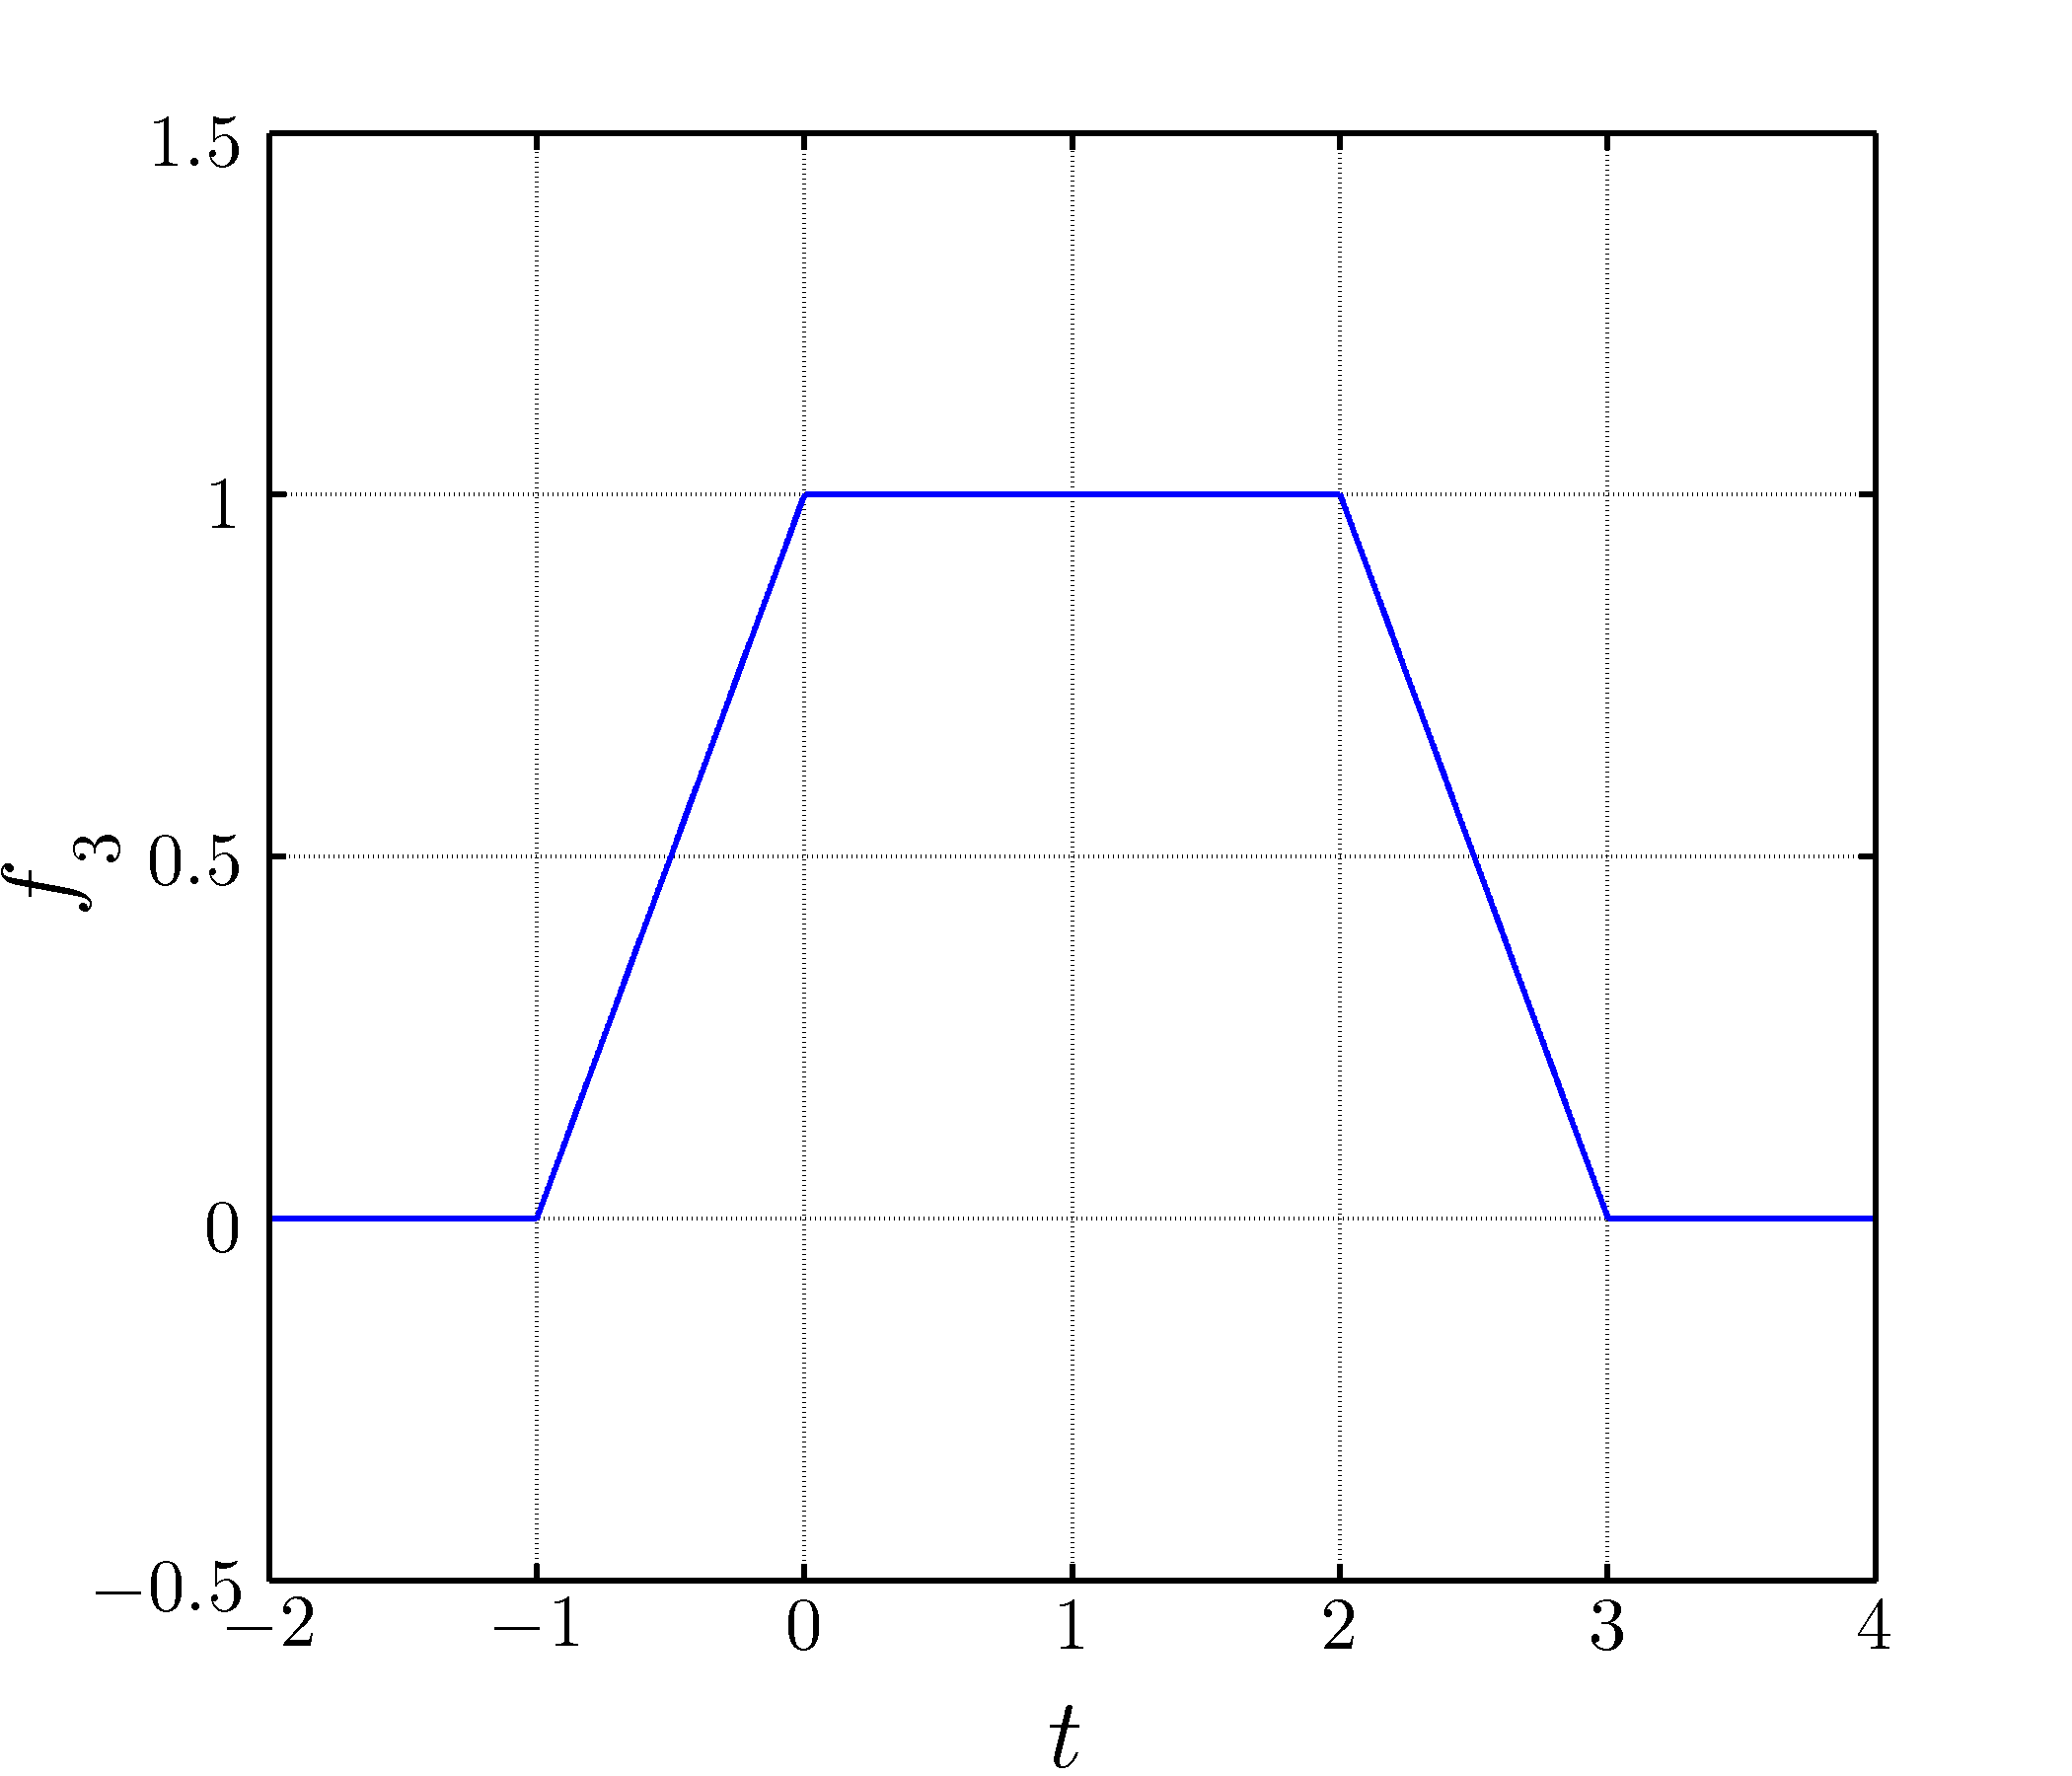
\includegraphics[width=\textwidth-30pt]{./laboratorio_4/problema01_f3.png}
              \end{flushright}
            \end{figure}\vspace{-1.0em}
        \end{enumerate}
      \end{minipage}%
      \begin{minipage}[t]{0.5\textwidth}
        \begin{enumerate}[label=\alph*)]
          \setcounter{enumi}{3}
          \item $f_4\left(t\right)$
            \vspace{-1.0em}
            \begin{figure}[H]
              \begin{flushright}
                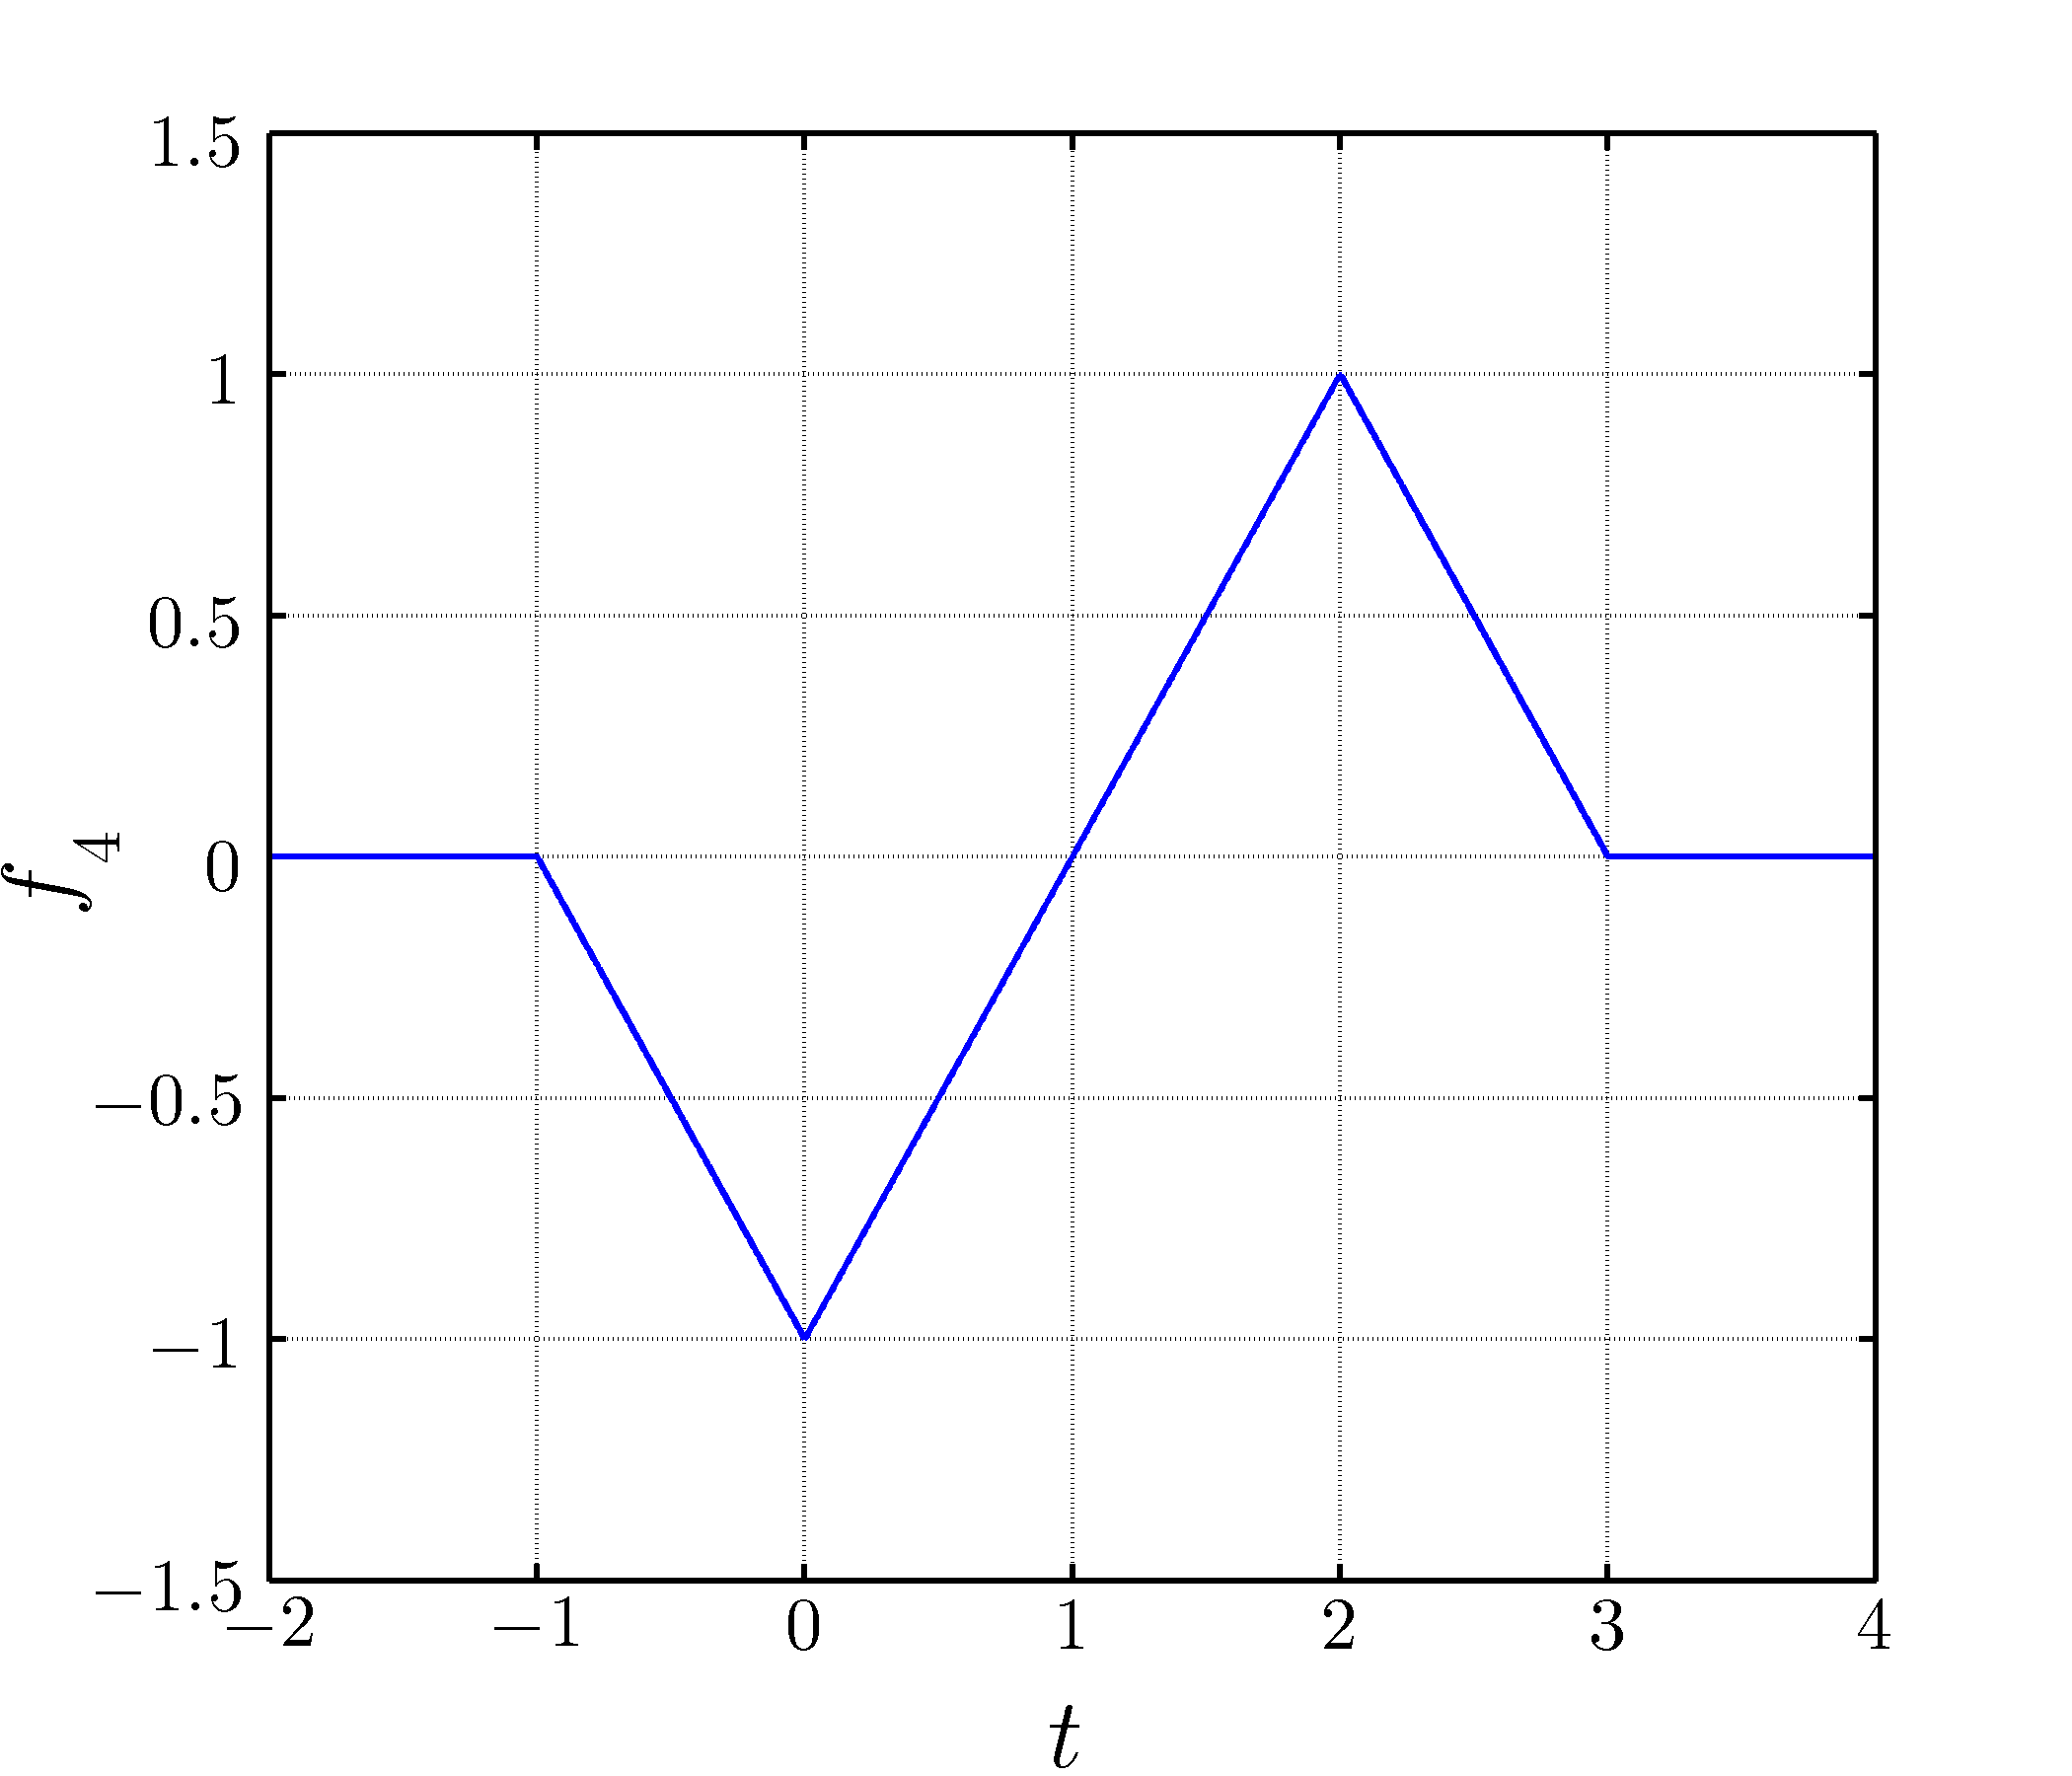
\includegraphics[width=\textwidth-30pt]{./laboratorio_4/problema01_f4.png}
              \end{flushright}
            \end{figure}\vspace{-1.0em}
        \end{enumerate}
      \end{minipage}%

      \noindent \emph{Nota}: $G$ es la función compuerta unitaria.

    \subsubsection*{Solución}
      \floatsetup[figure]{
        capposition=top,
        style=ruled,
      }

      \noindent Definimos la función compuerta unitaria, $G$, empleando la función
      $\Theta$ de Heaviside de la siguiente manera

      \begin{equation*}
         G\left(t\right) = \Theta\left(t + \frac{1}{2}\right) -
                           \Theta\left(t - \frac{1}{2}\right).
      \end{equation*}

      \noindent Empleando la función $G$ podemos definir la función triángulo,
      $\Lambda$, como

      \begin{equation*}
         \Lambda\left(t\right) = \left(1 - 2\left|t\right|\right)G\left(t\right)
      \end{equation*}

      \noindent Con estas dos funciones definimos las funciones $f_3$ y $f_4$
      como

      \begin{equation*}
         f_3\left(t\right) = \Lambda\left(\frac{1}{2}t\right) +
                             \Lambda\left(\frac{1}{2}t + \frac{1}{2}\right) +
                             \Lambda\left(\frac{1}{2}t + 1\right),
      \end{equation*}

      \begin{equation*}
         f_4\left(t\right) = - \Lambda\left(\frac{1}{2}t\right) +
                               \Lambda\left(\frac{1}{2}t + 1\right).
      \end{equation*}

      \noindent Empleando la transformada de Fourier definida por

      \begin{equation*}
        \mathcal{F}\left(f,t|\omega\right) = \widehat{f}\left(\omega\right) = \int_{-\infty}^{\infty}f\left(t\right)\exp\left(- i \omega t\right)dt
      \end{equation*}

      \noindent y que

      \begin{equation*}
        \widehat{G}\left(\omega\right) = \mathrm{sinc}\left(\frac{\omega}{2}\right),
      \end{equation*}

      \begin{equation*}
        \widehat{\Lambda}\left(\omega\right) = \frac{1}{2}\mathrm{sinc}^{2}\left(\frac{\omega}{4}\right),
      \end{equation*}

      \noindent tenemos

      \begin{enumerate}[label=\alph*)]
        \item $\widehat{f}_{1}\left(\omega\right)$
          \begin{equation*}
            \begin{split}
              \widehat{f}_{1}\left(\omega\right) & = \mathcal{F}\left(G,\left.\frac{t}{2}\right|\omega\right) - \mathcal{F}\left(G,t|\omega\right) \\
                                                 & = 2\mathcal{F}\left(G,t|2\omega\right) - \mathcal{F}\left(G,t|\omega\right) \\
                                                 & = 2\mathrm{sinc}\left(\omega\right) - \mathrm{sinc}\left(\frac{\omega}{2}\right)
            \end{split}
          \end{equation*}

        \item $\widehat{f}_{2}\left(\omega\right)$
          \begin{equation*}
            \begin{split}
              \widehat{f}_{2}\left(\omega\right) & = 5\mathcal{F}\left(G,t-1|\omega\right) - \mathcal{F}\left(G,t+1|\omega\right) \\
                                                 & = 5\exp\left(-i \omega\right)\mathcal{F}\left(G,t|\omega\right) - \exp\left(i \omega\right)\mathcal{F}\left(G,t|\omega\right) \\
                                                 & = 2\mathrm{sinc}\left(\frac{\omega}{2}\right)\left(2\cos\left(\omega\right) - 3i\sin\left(\omega\right) \right)
            \end{split}
          \end{equation*}

        \item $\widehat{f}_{3}\left(\omega\right)$
          \begin{equation*}
            \begin{split}
              \widehat{f}_{3}\left(\omega\right) & = \mathcal{F}\left(\Lambda,\left.\frac{t}{2}\right|\omega\right) + \mathcal{F}\left(\Lambda,\left.\frac{t}{2} + \frac{1}{2}\right|\omega\right) + \mathcal{F}\left(\Lambda,\left.\frac{t}{2} + 1\right|\omega\right) \\
                                                 & = 2 \mathcal{F}\left(\Lambda,t| 2 \omega\right) + 2 \exp\left(i \omega\right) \mathcal{F}\left(\Lambda,t|2 \omega\right) + 2 \exp\left(2 i \omega\right) \mathcal{F}\left(\Lambda,t| 2\omega\right) \\
                                                 & = \mathrm{sinc}^{2}\left(\frac{\omega}{2}\right) + \exp\left(i \omega\right) \mathrm{sinc}^{2}\left(\frac{\omega}{2}\right) + \exp\left(2 i \omega\right) \mathrm{sinc}^{2}\left(\frac{\omega}{2}\right) \\
                                                 & = \left(1 + 2 \cos\left(\omega\right) \right)\exp\left(i \omega\right)\mathrm{sinc}^{2}\left(\frac{\omega}{2}\right)
            \end{split}
          \end{equation*}

        \item $\widehat{f}_{1}\left(\omega\right)$
          \begin{equation*}
            \begin{split}
              \widehat{f}_{3}\left(\omega\right) & = - \mathcal{F}\left(\Lambda,\left.\frac{t}{2}\right|\omega\right) + \mathcal{F}\left(\Lambda,\left.\frac{t}{2} + 1\right|\omega\right) \\
                                                 & = - 2 \mathcal{F}\left(\Lambda,t| 2 \omega\right) + 2 \exp\left(2 i \omega\right) \mathcal{F}\left(\Lambda,t| 2\omega\right) \\
                                                 & = - \mathrm{sinc}^{2}\left(\frac{\omega}{2}\right) + \exp\left(2 i \omega\right) \mathrm{sinc}^{2}\left(\frac{\omega}{2}\right) \\
                                                 & = \left(\exp\left(2 i \omega\right) - 1\right)\mathrm{sinc}^{2}\left(\frac{\omega}{2}\right)
            \end{split}
          \end{equation*}
      \end{enumerate}

      \noindent En \textsc{Matlab} implementamos las funciones

      \begin{listing}[H]
        \caption{Función compuerta unitaria, $G\left(t\right)$.}
        \label{script01A}
        \inputminted{matlab}{./laboratorio_4/gate.m}
      \end{listing}\vspace{-1.0em}

      \begin{listing}[H]
        \caption{Función triángulo, $\Lambda\left(t\right)$.}
        \label{script01B}
        \inputminted{matlab}{./laboratorio_4/triangle.m}
      \end{listing}\vspace{-1.0em}

      \begin{listing}[H]
        \caption{Función $f_1\left(t\right)$.}
        \label{script01C}
        \inputminted{matlab}{./laboratorio_4/p1_f1.m}
      \end{listing}\vspace{-1.0em}

      \begin{listing}[H]
        \caption{Función $f_2\left(t\right)$.}
        \label{script01D}
        \inputminted{matlab}{./laboratorio_4/p1_f2.m}
      \end{listing}\vspace{-1.0em}

      \begin{listing}[H]
        \caption{Función $f_3\left(t\right)$.}
        \label{script01E}
        \inputminted{matlab}{./laboratorio_4/p1_f3.m}
      \end{listing}\vspace{-1.0em}

      \begin{listing}[H]
        \caption{Función $f_4\left(t\right)$.}
        \label{script01F}
        \inputminted{matlab}{./laboratorio_4/p1_f4.m}
      \end{listing}\vspace{-1.0em}

      \begin{figure}[H]
        \caption{Gráfico de la función $f_1$ y su espectro de potencia normalizado.}
        \label{script01Afigure}
        \begin{center}
          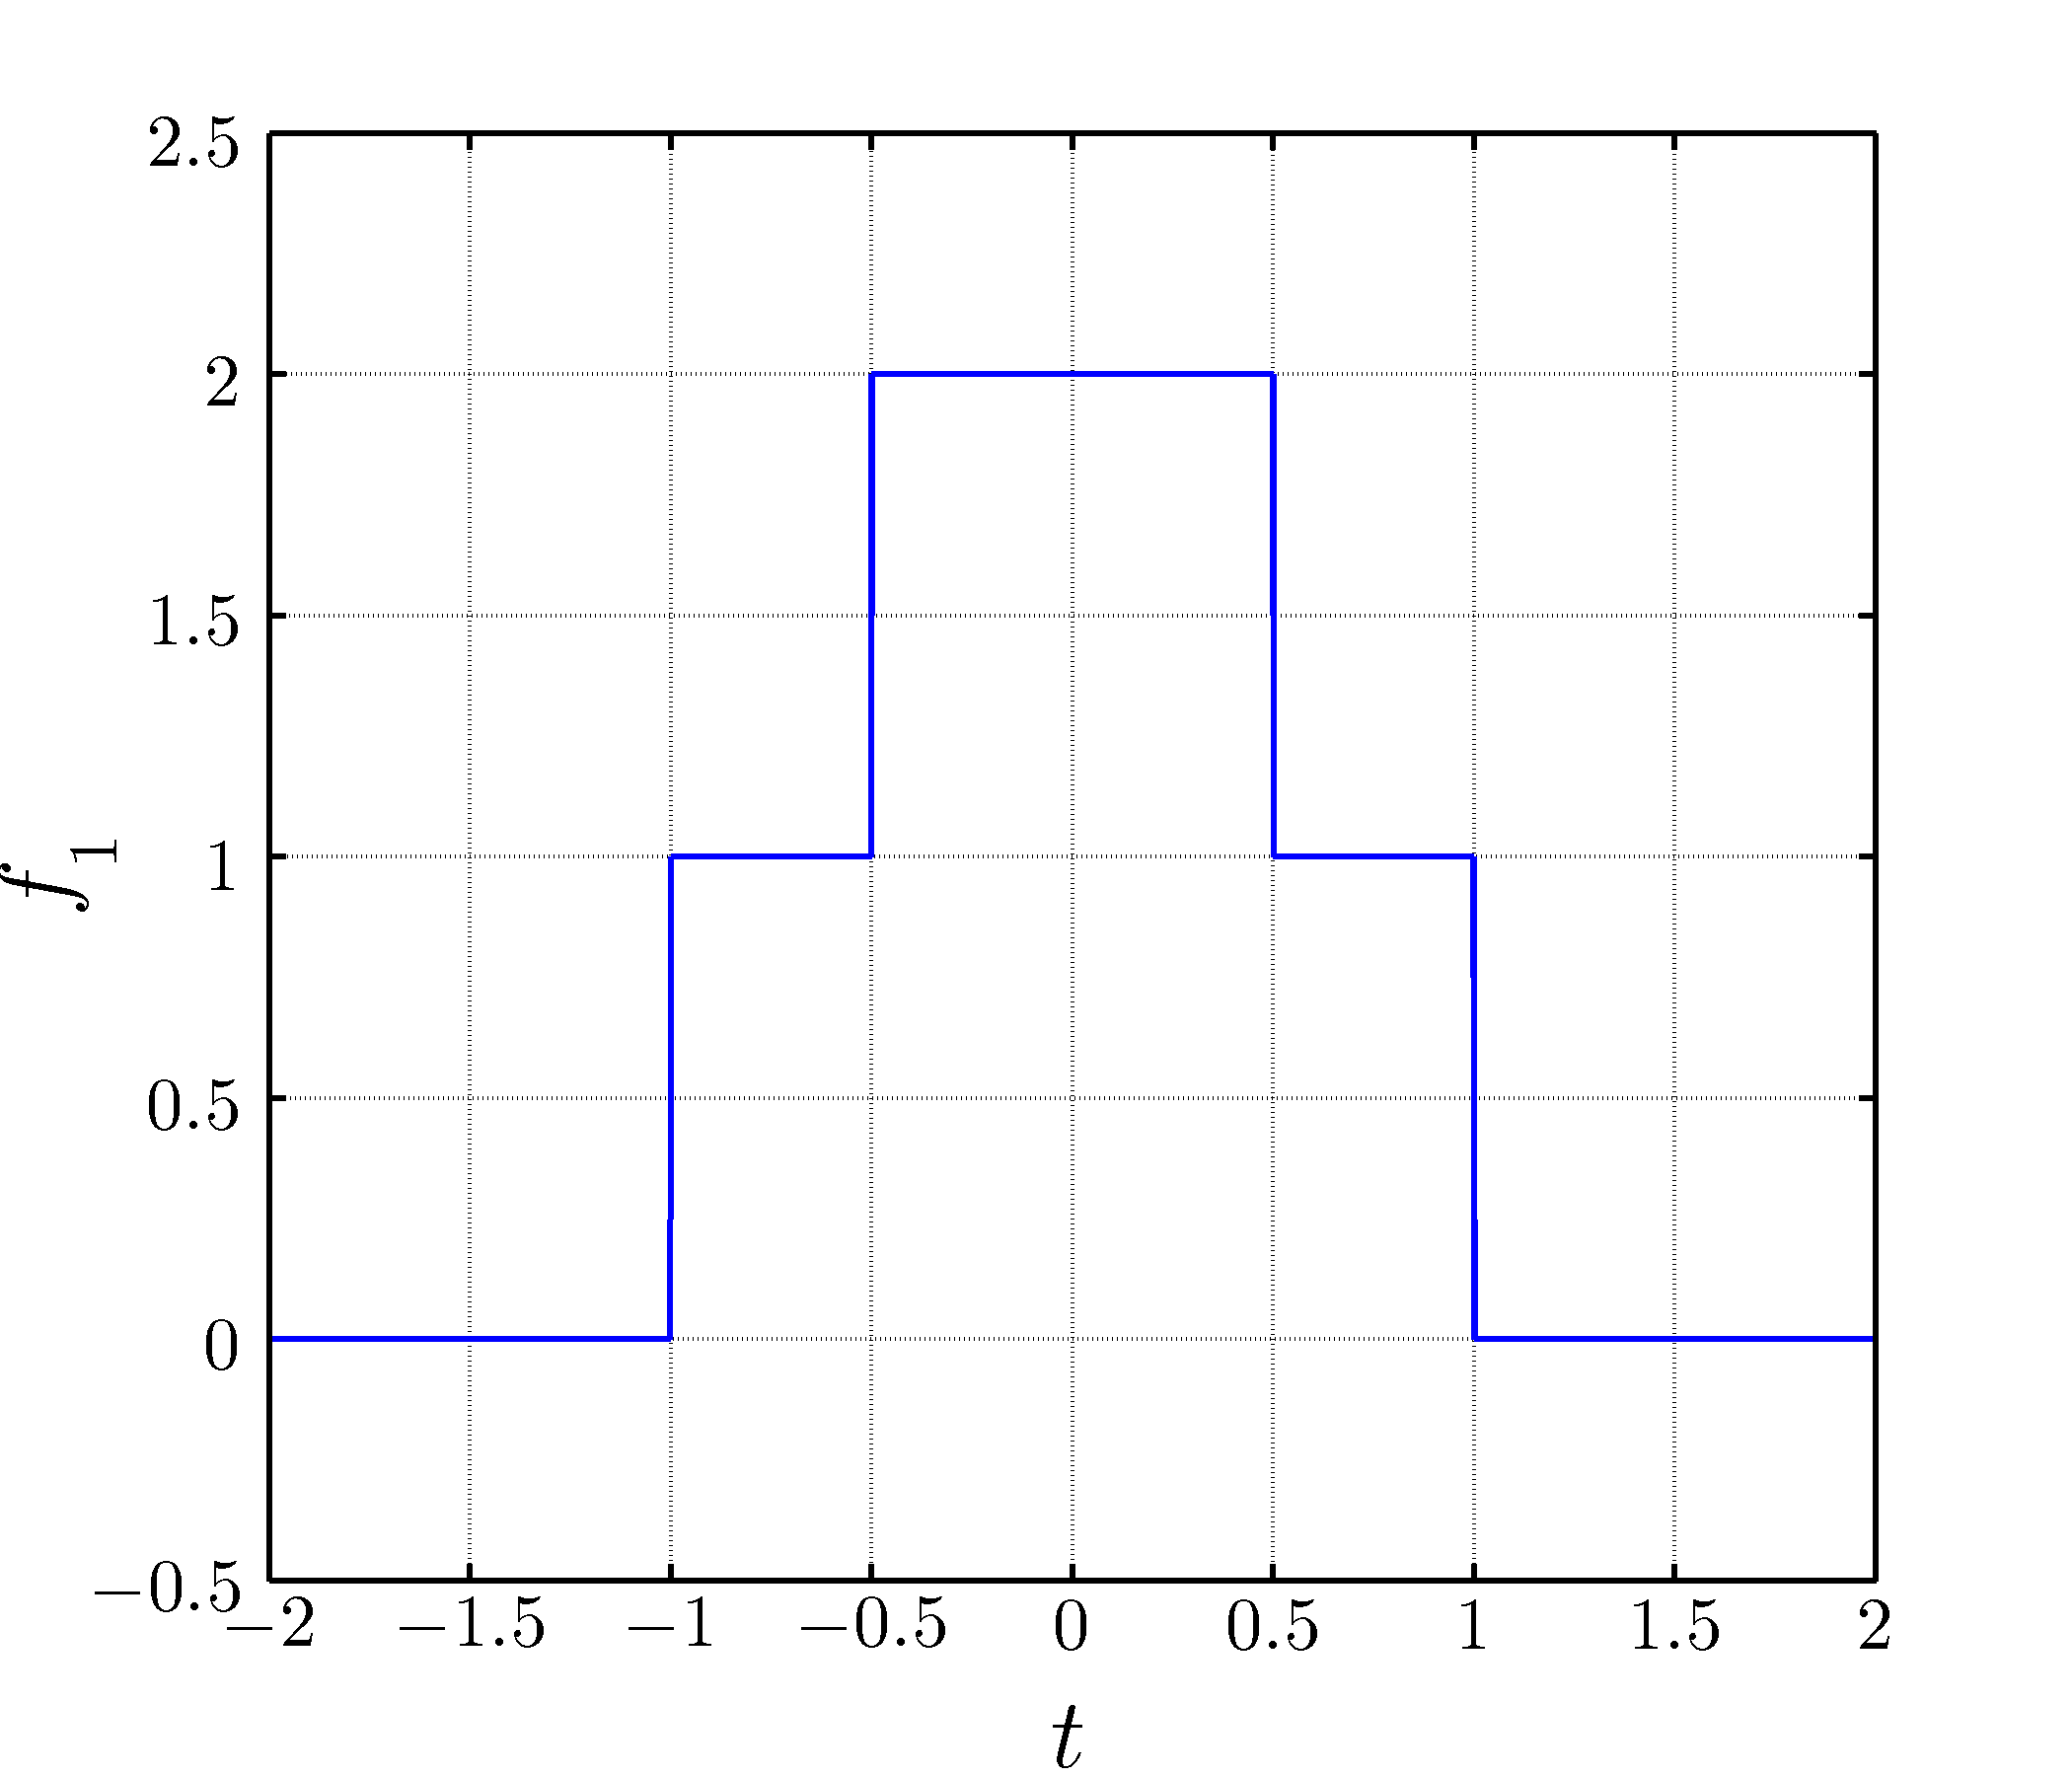
\includegraphics[width=0.45\textwidth]{./laboratorio_4/problema01_f1.png}
          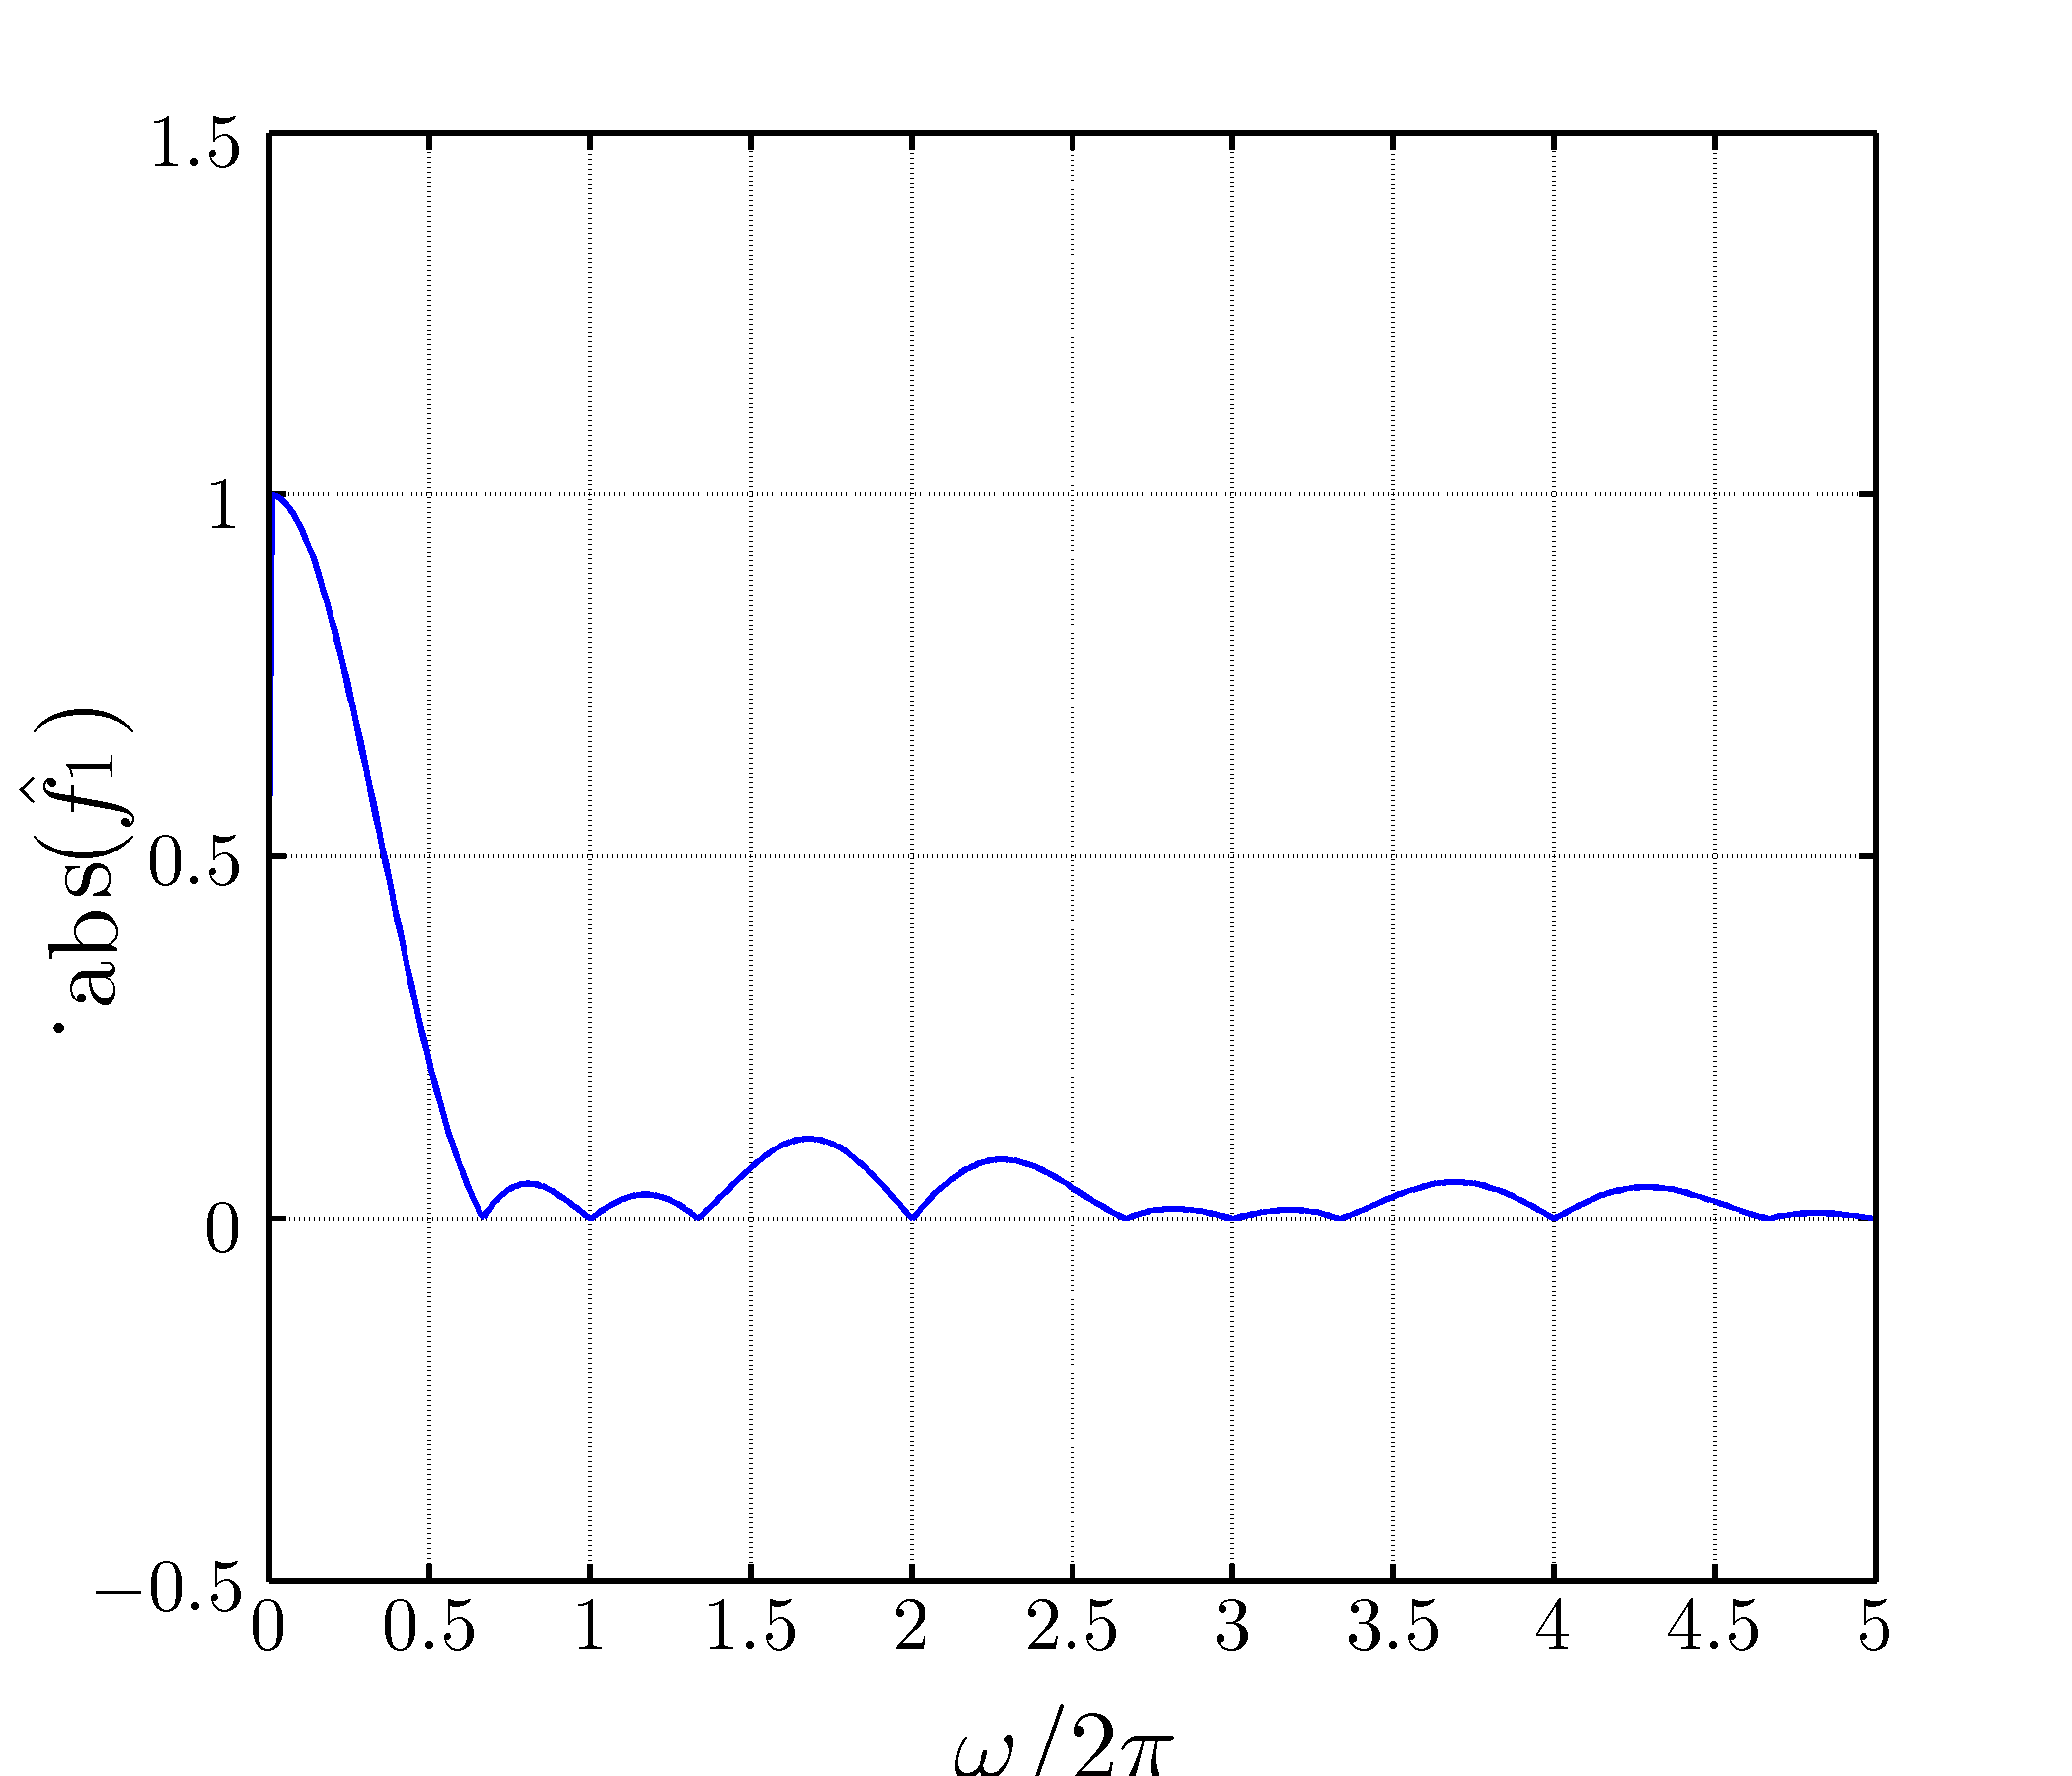
\includegraphics[width=0.45\textwidth]{./laboratorio_4/problema01_F1.png}
        \end{center}
      \end{figure}

      \begin{figure}[H]
        \caption{Gráfico de la función $f_2$ y su espectro de potencia normalizado.}
        \label{script01Bfigure}
        \begin{center}
          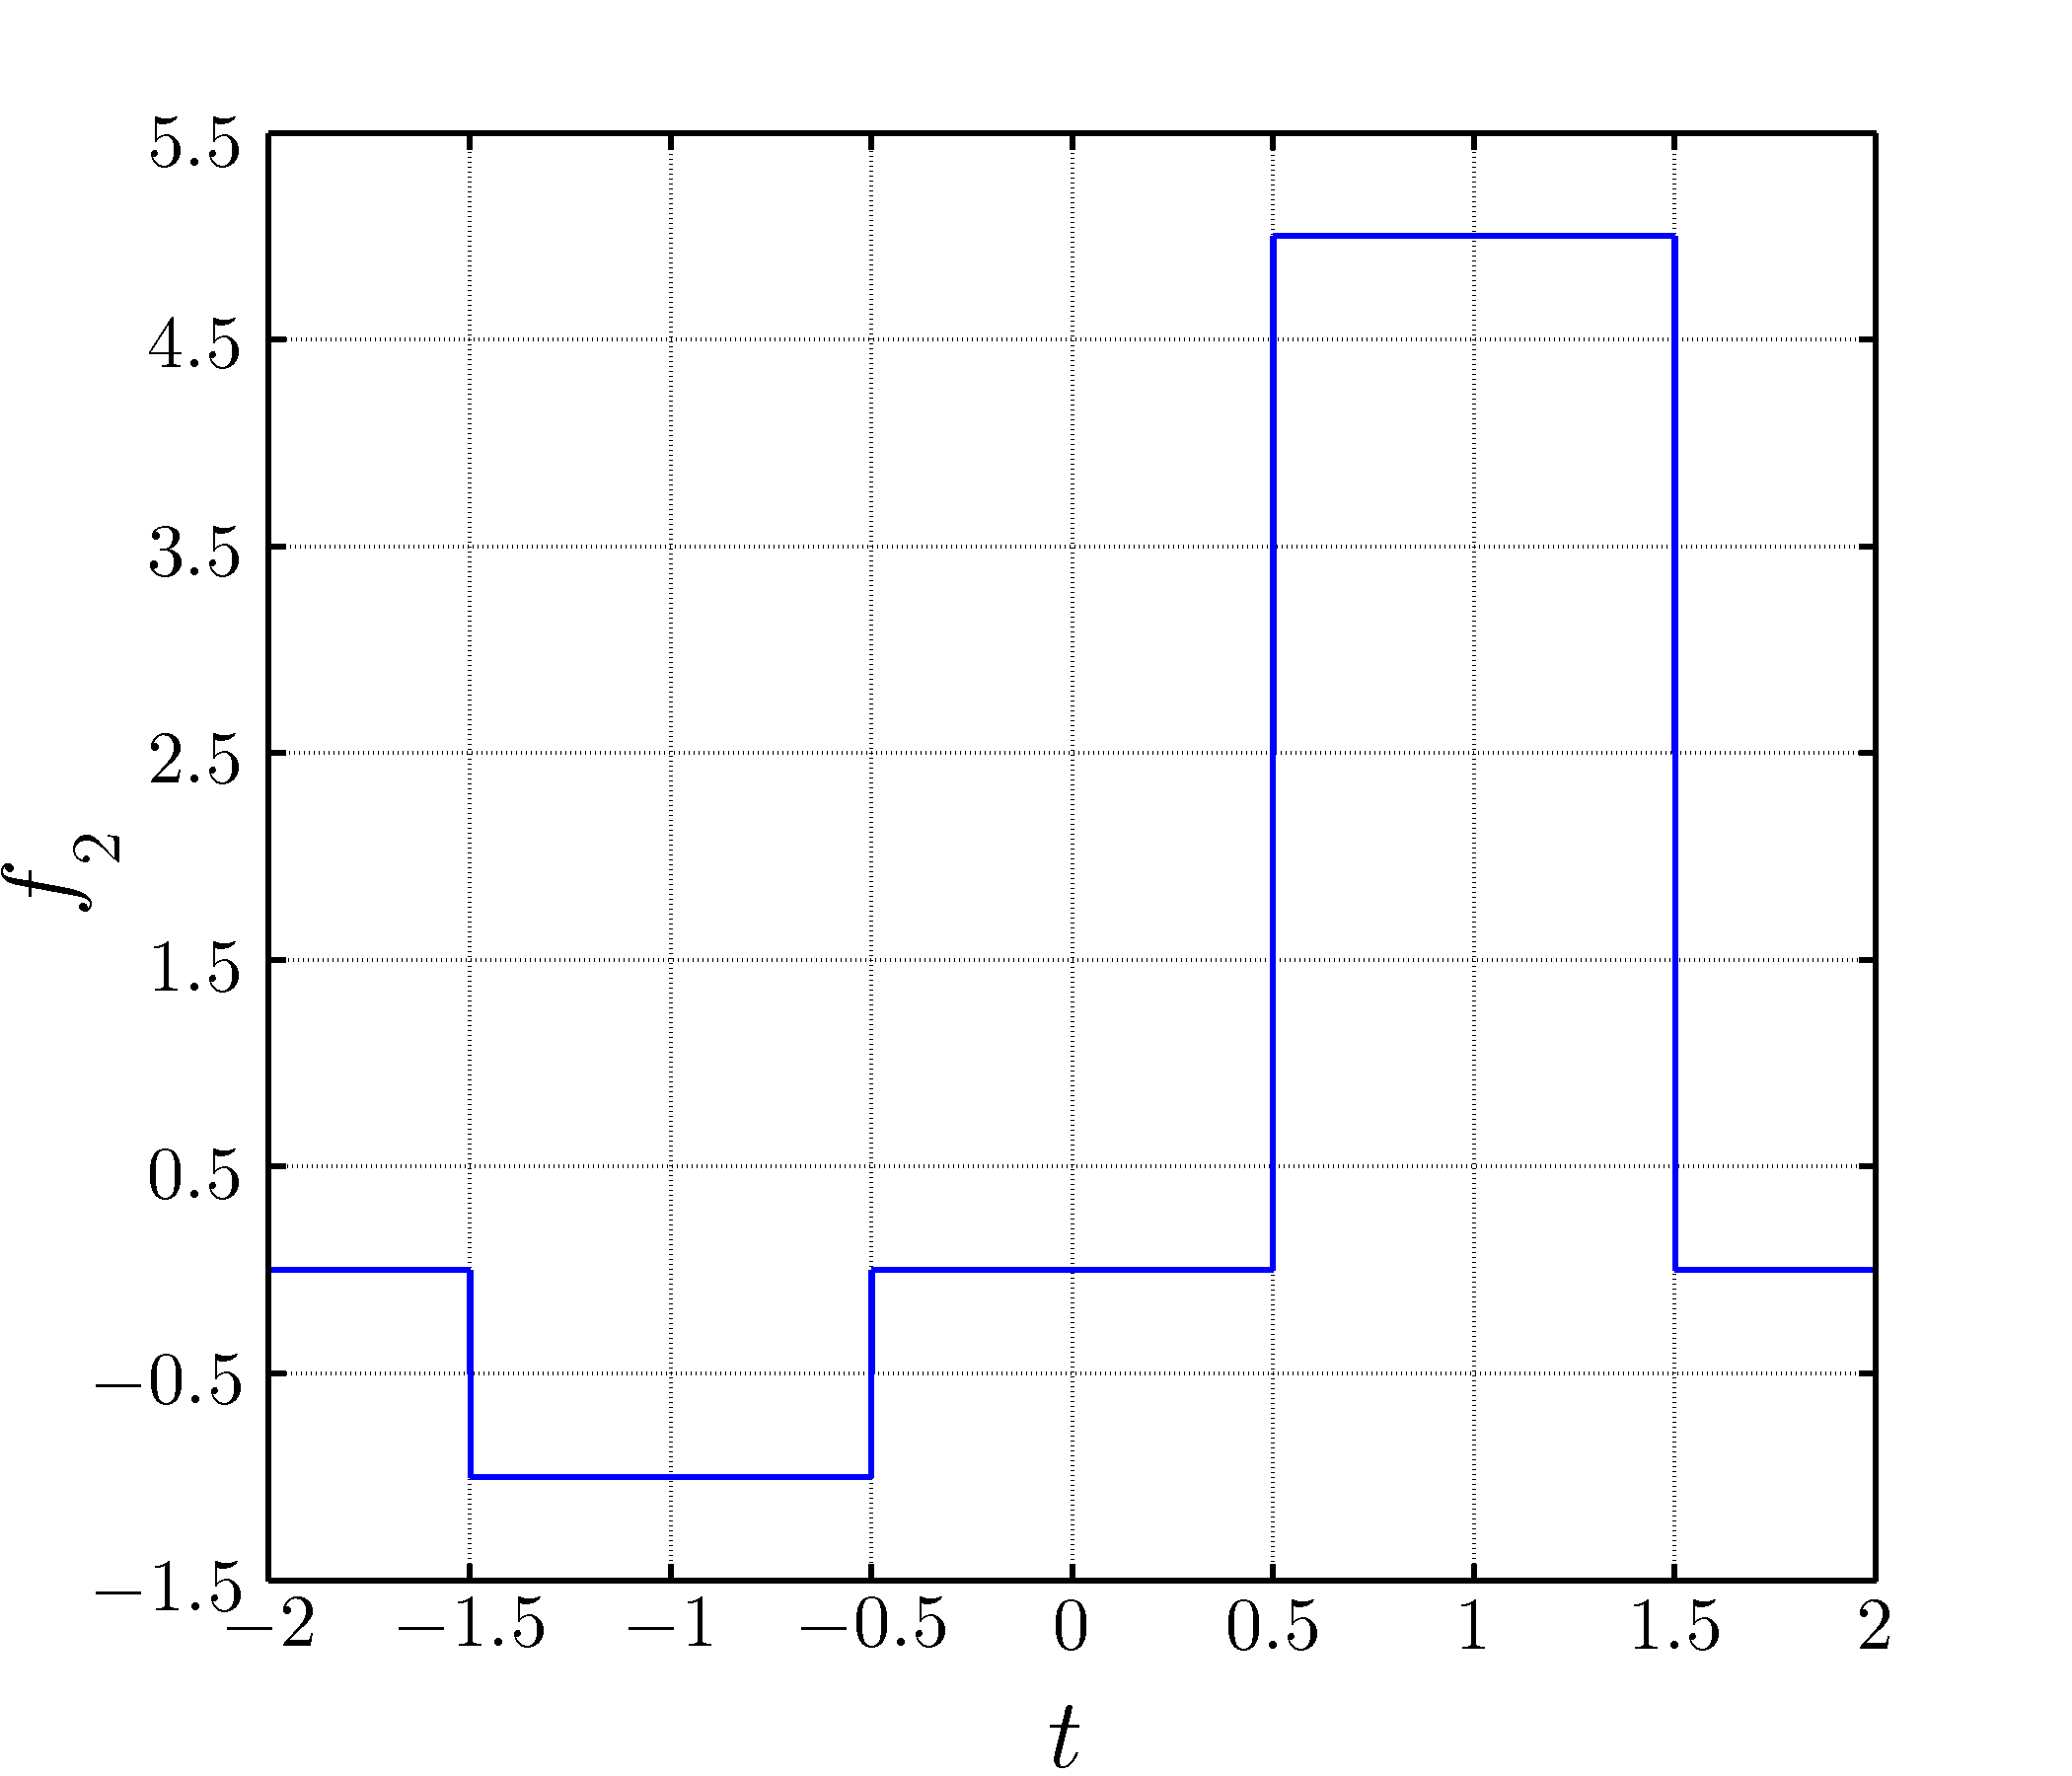
\includegraphics[width=0.45\textwidth]{./laboratorio_4/problema01_f2.png}
          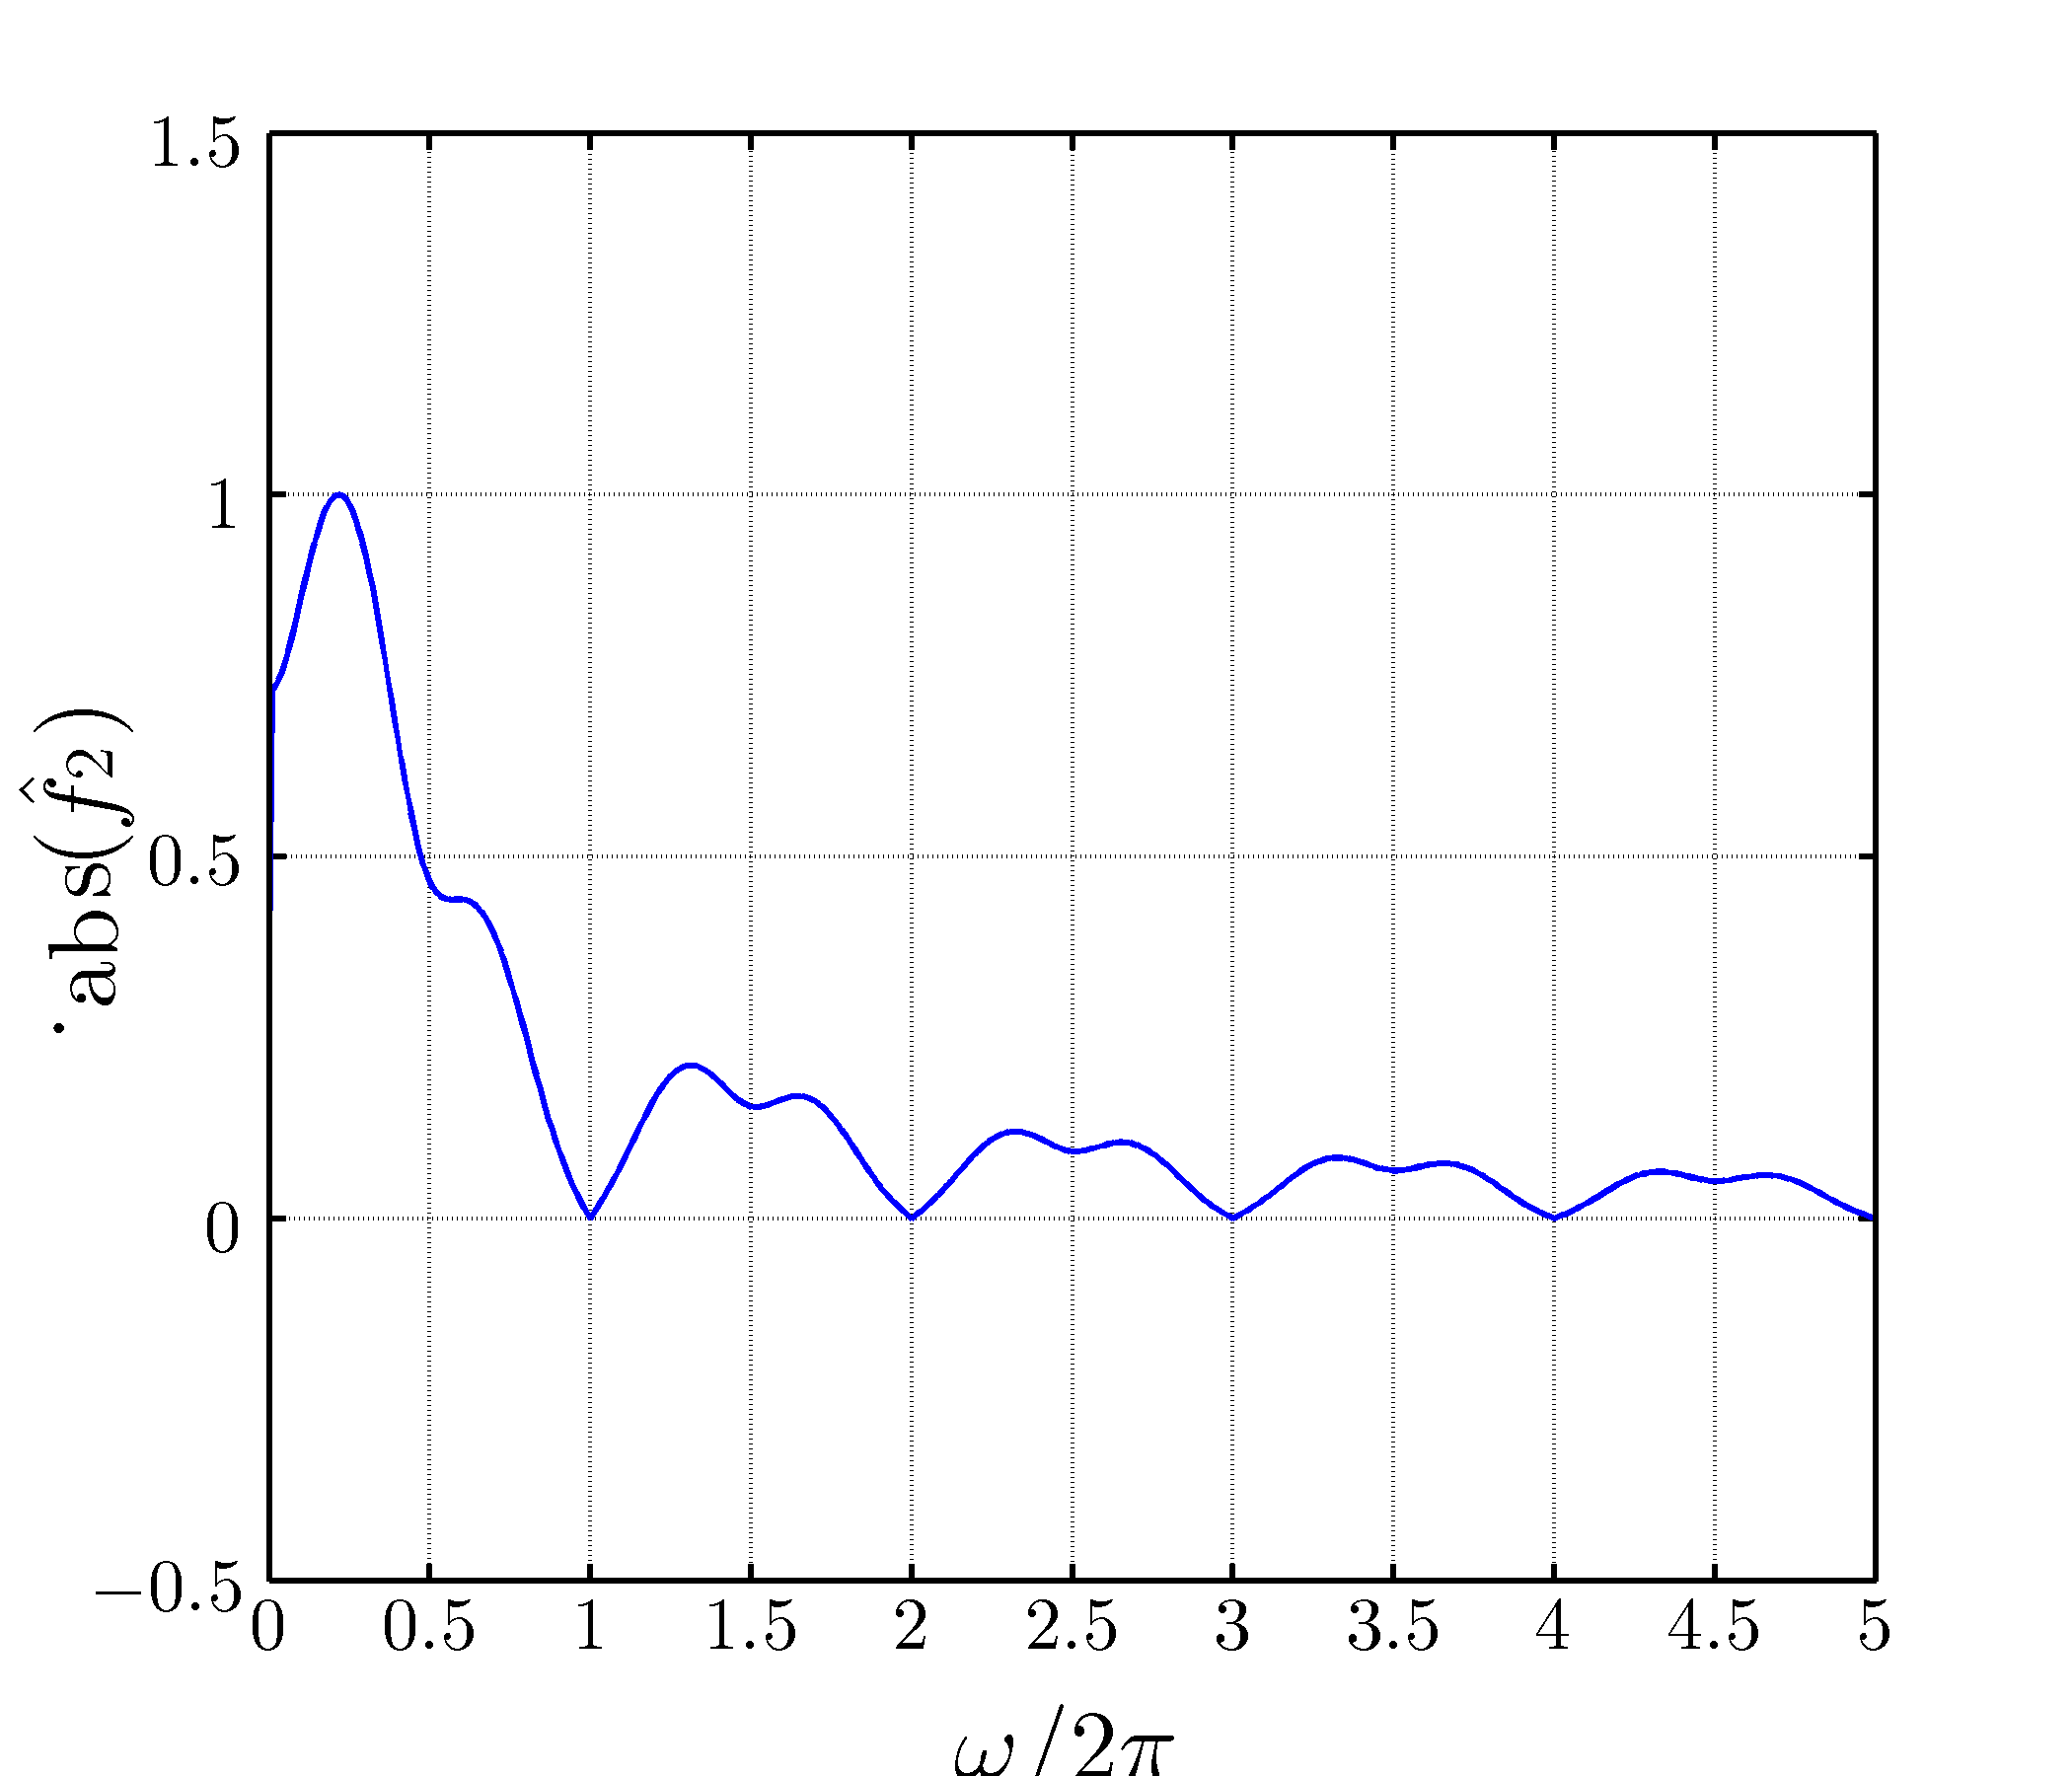
\includegraphics[width=0.45\textwidth]{./laboratorio_4/problema01_F2.png}
        \end{center}
      \end{figure}

      \begin{figure}[H]
        \caption{Gráfico de la función $f_3$ y su espectro de potencia normalizado.}
        \label{script01Cfigure}
        \begin{center}
          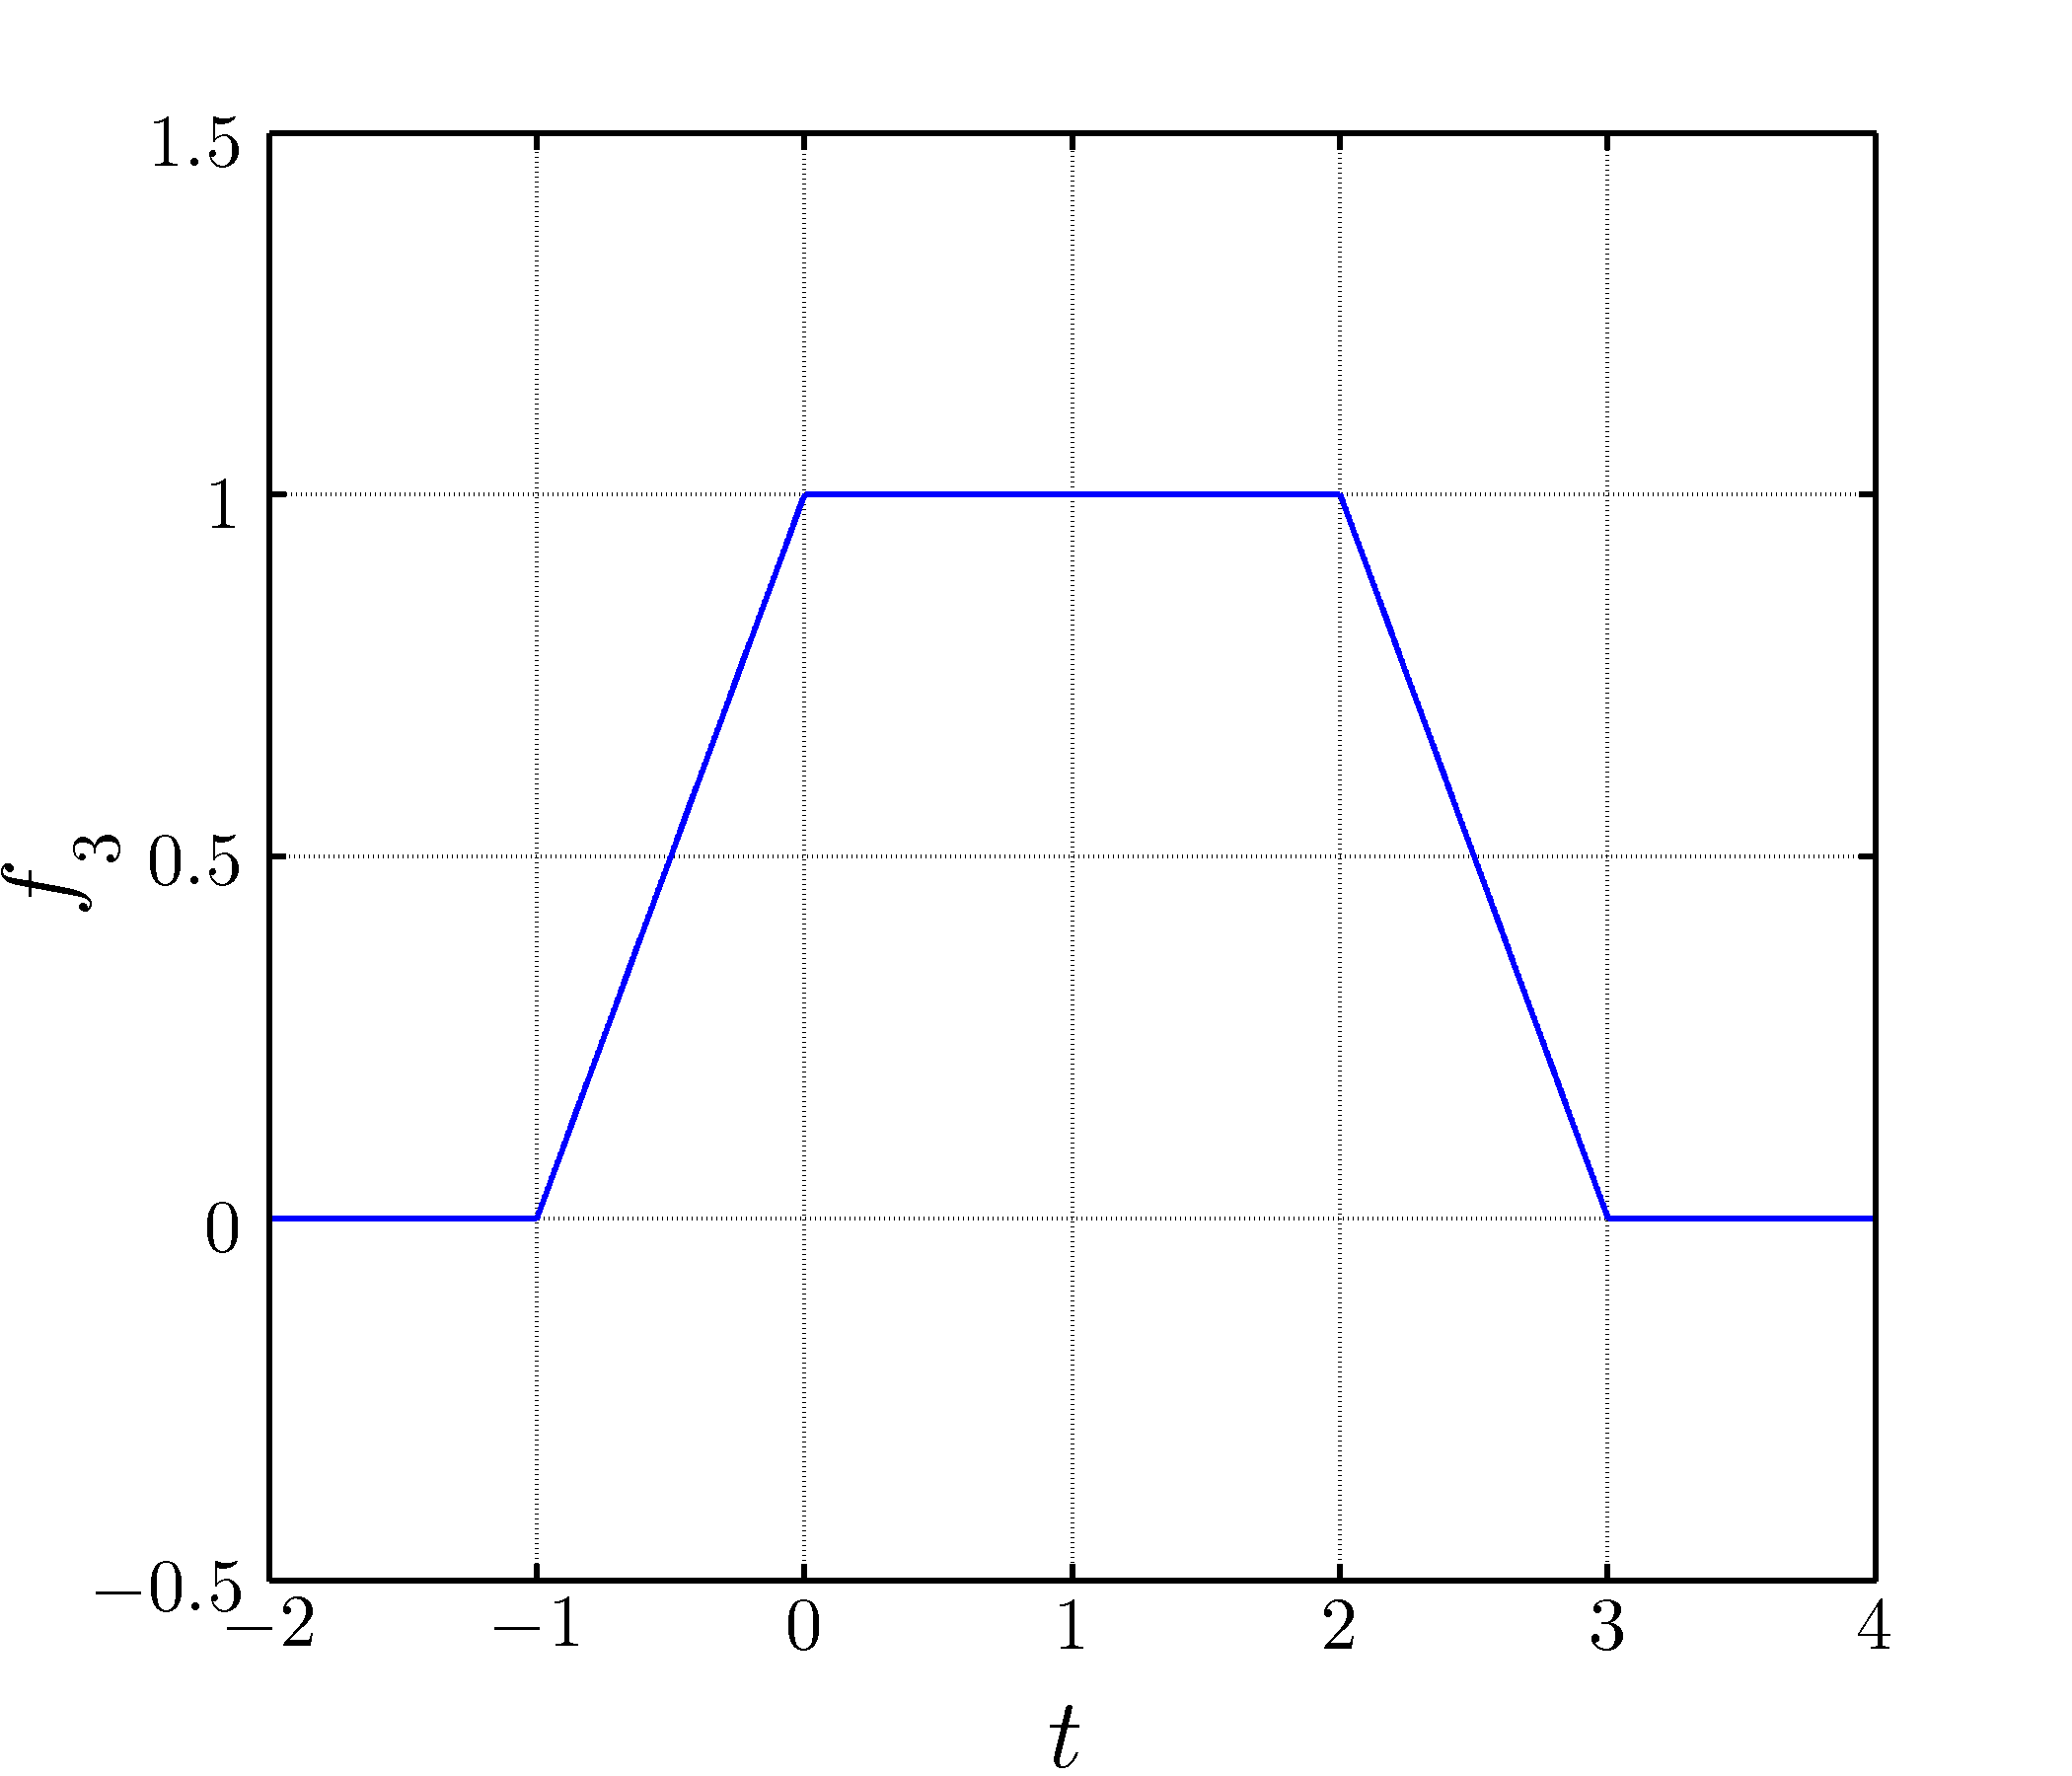
\includegraphics[width=0.45\textwidth]{./laboratorio_4/problema01_f3.png}
          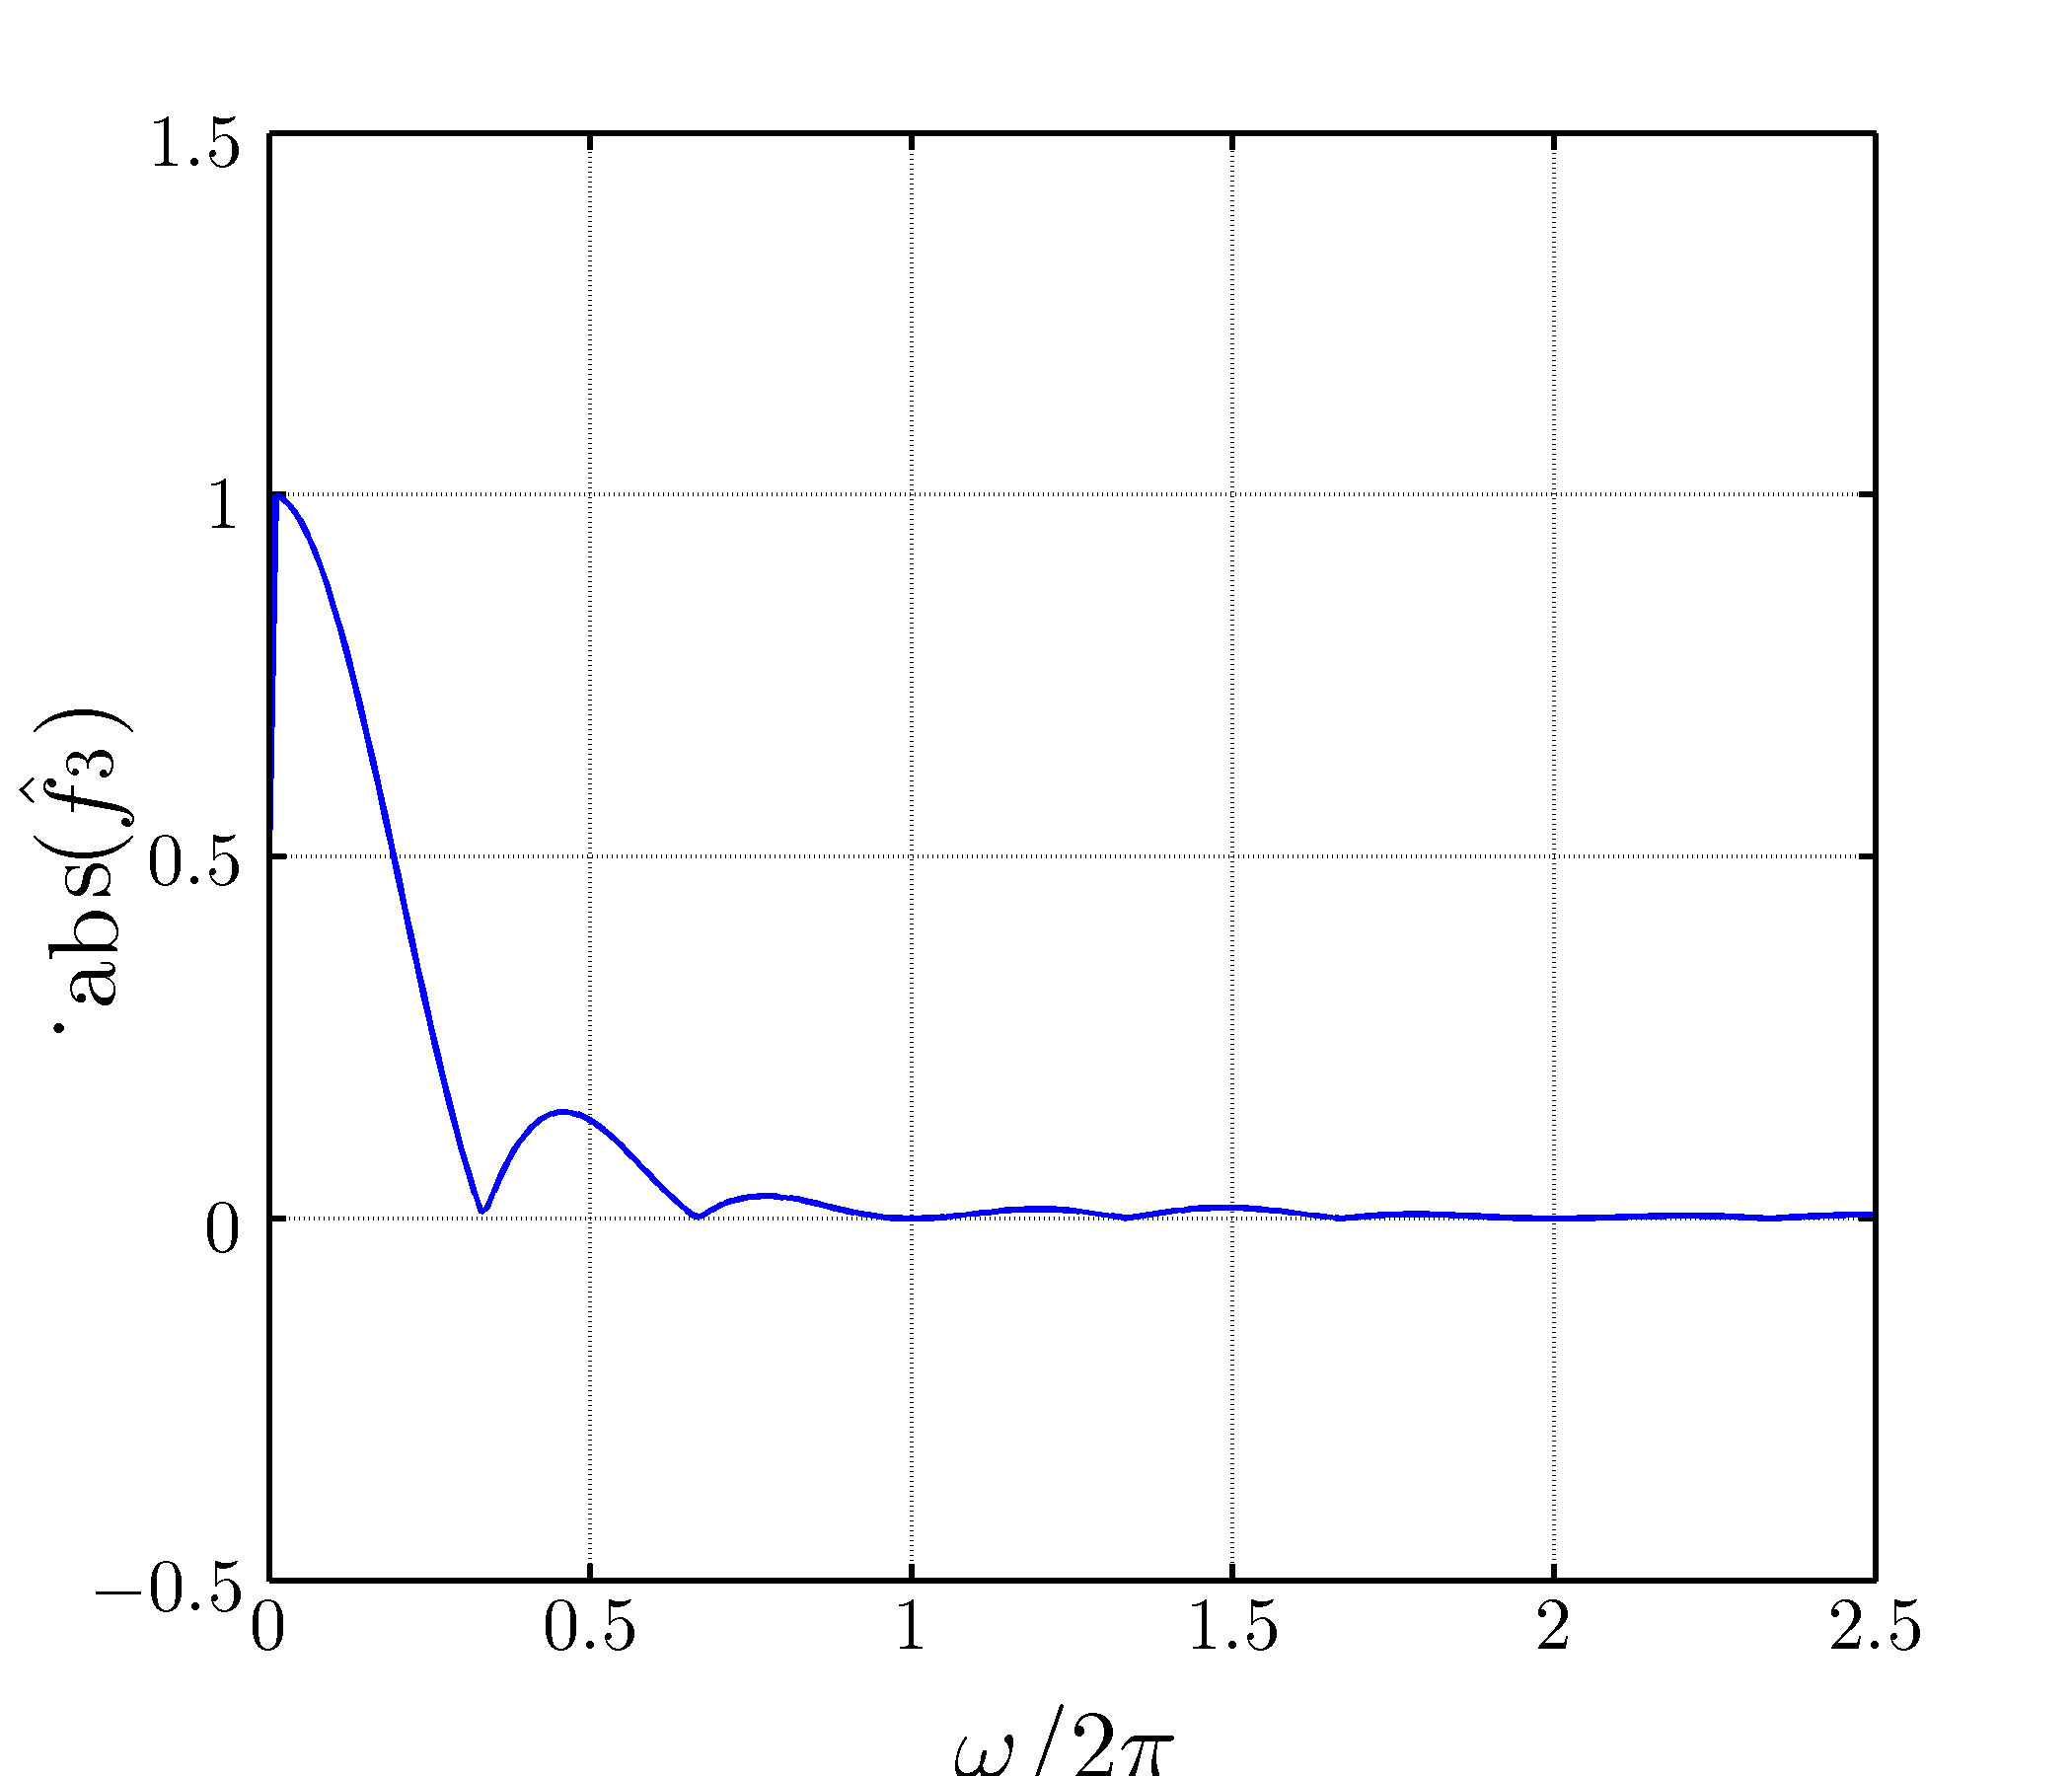
\includegraphics[width=0.45\textwidth]{./laboratorio_4/problema01_F3.png}
        \end{center}
      \end{figure}

      \begin{figure}[H]
        \caption{Gráfico de la función $f_1$ y su espectro de potencia normalizado.}
        \label{script01Dfigure}
        \begin{center}
          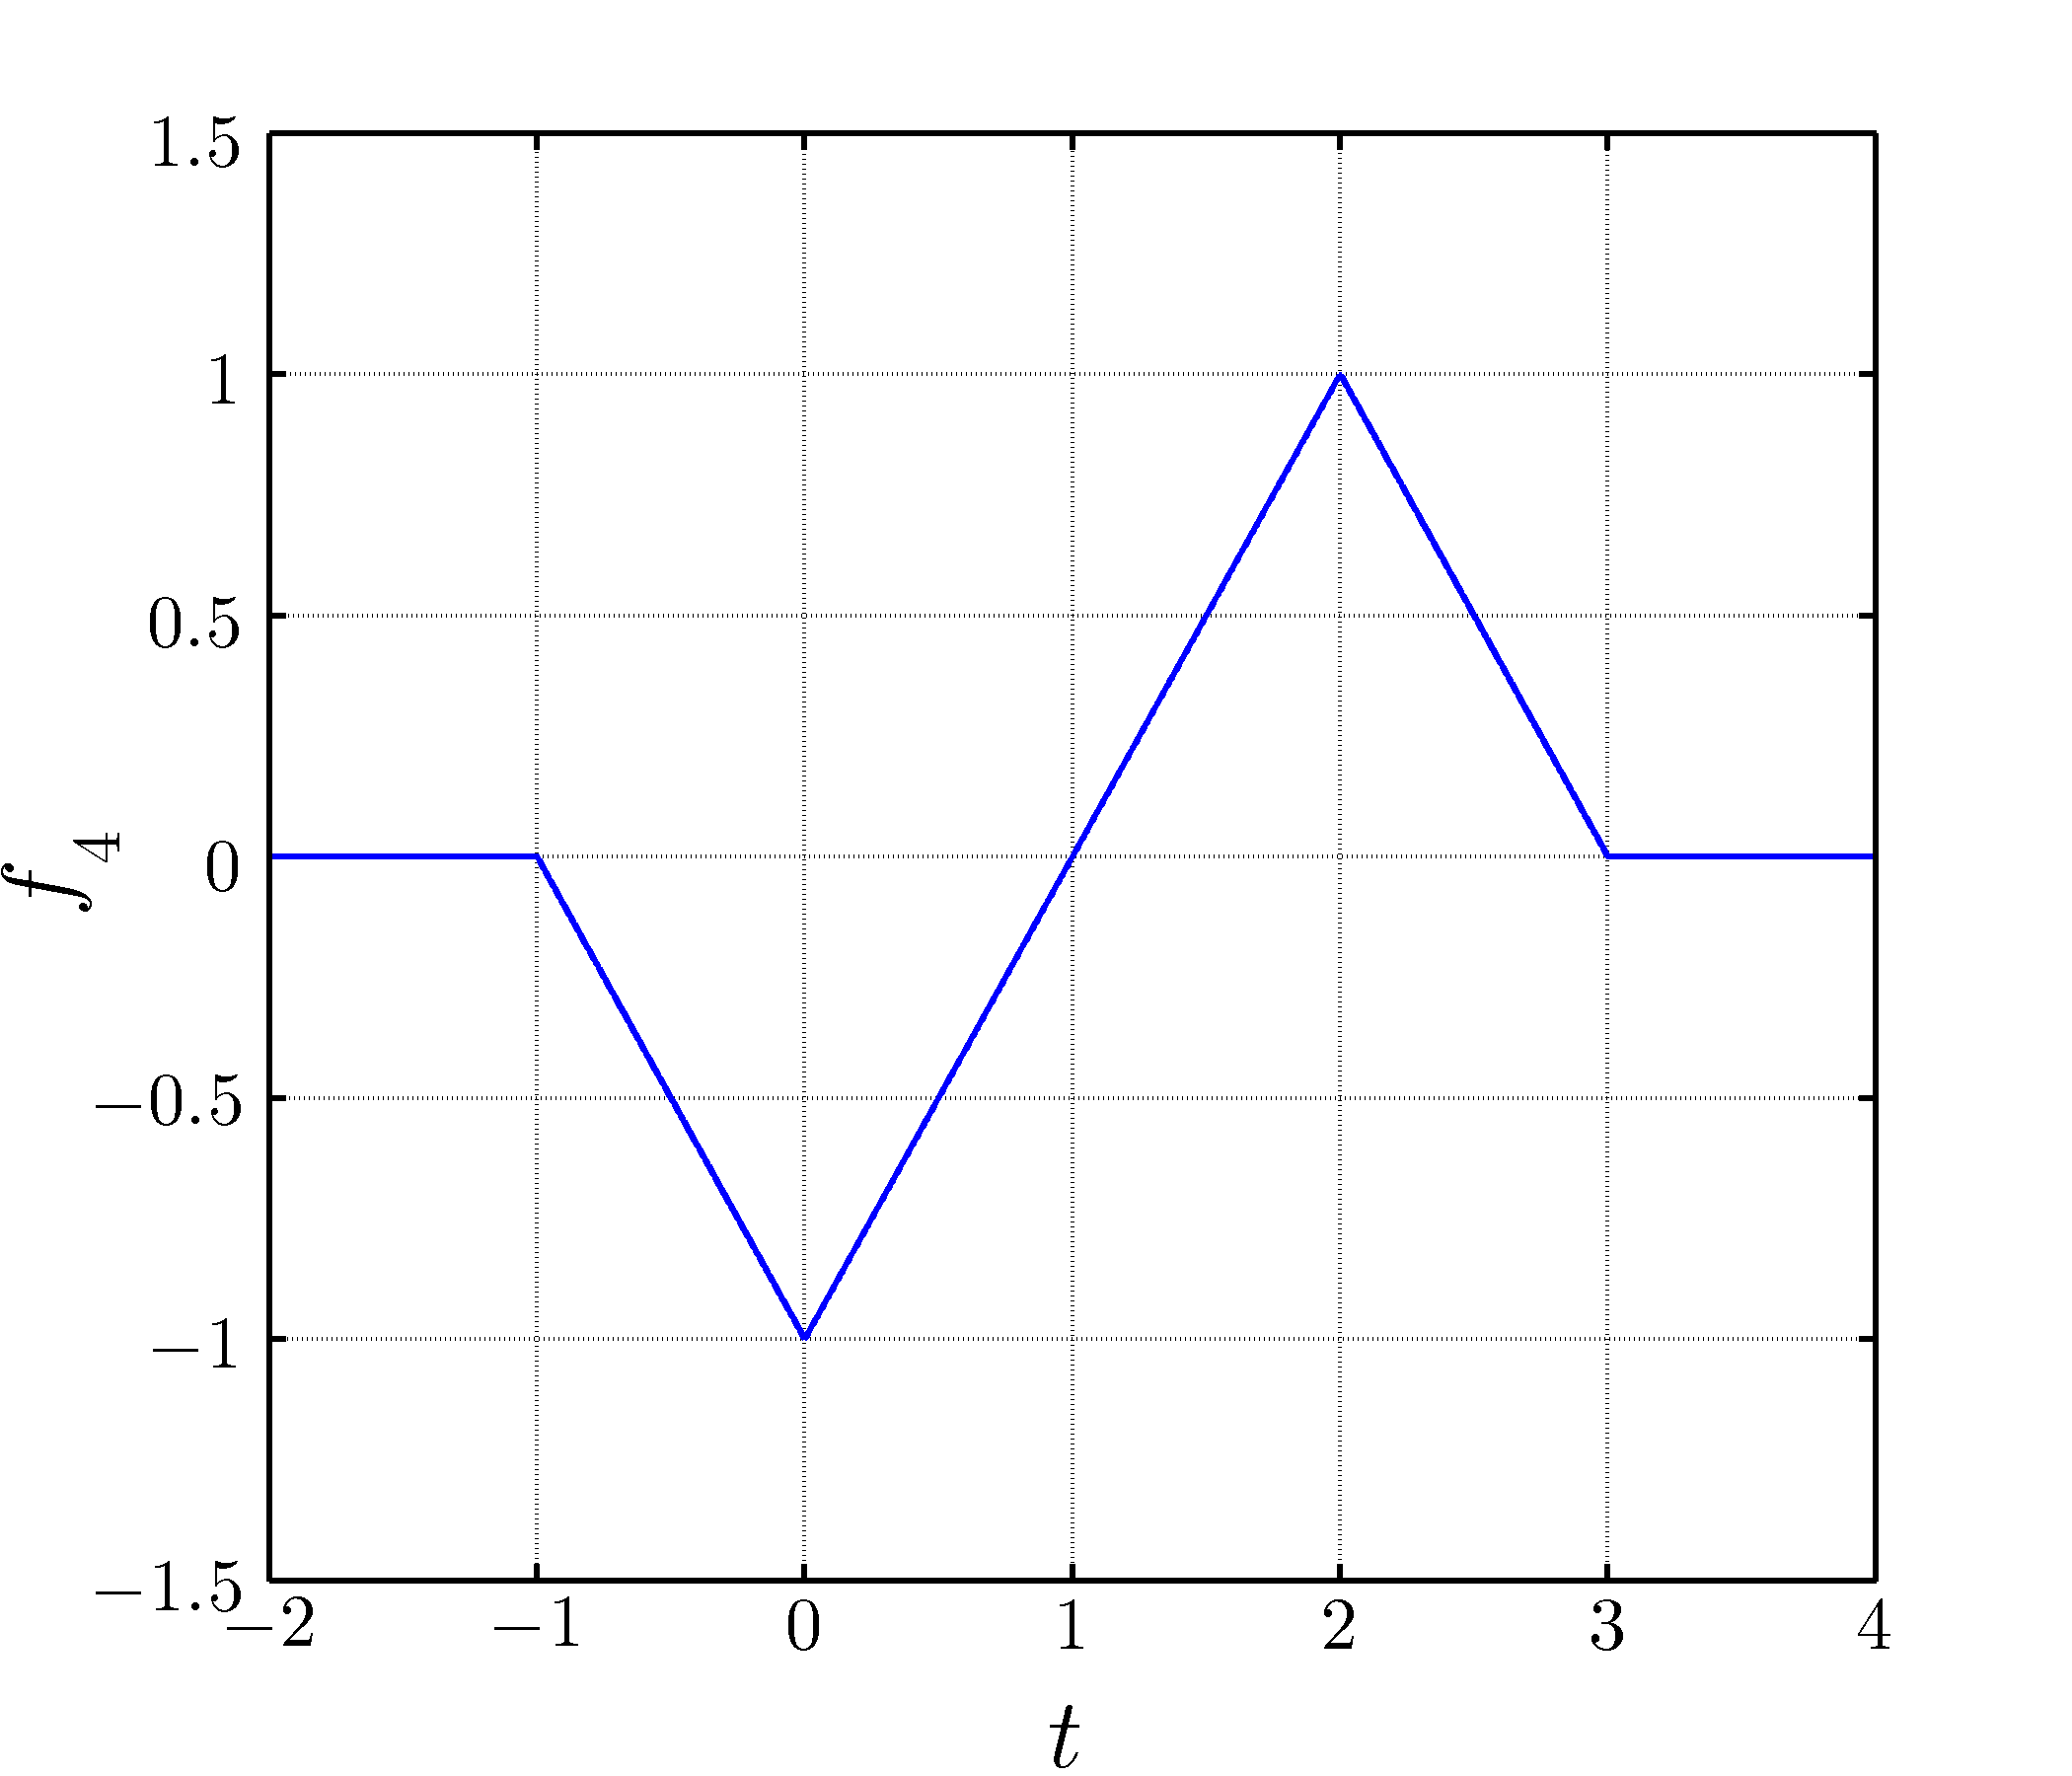
\includegraphics[width=0.45\textwidth]{./laboratorio_4/problema01_f4.png}
          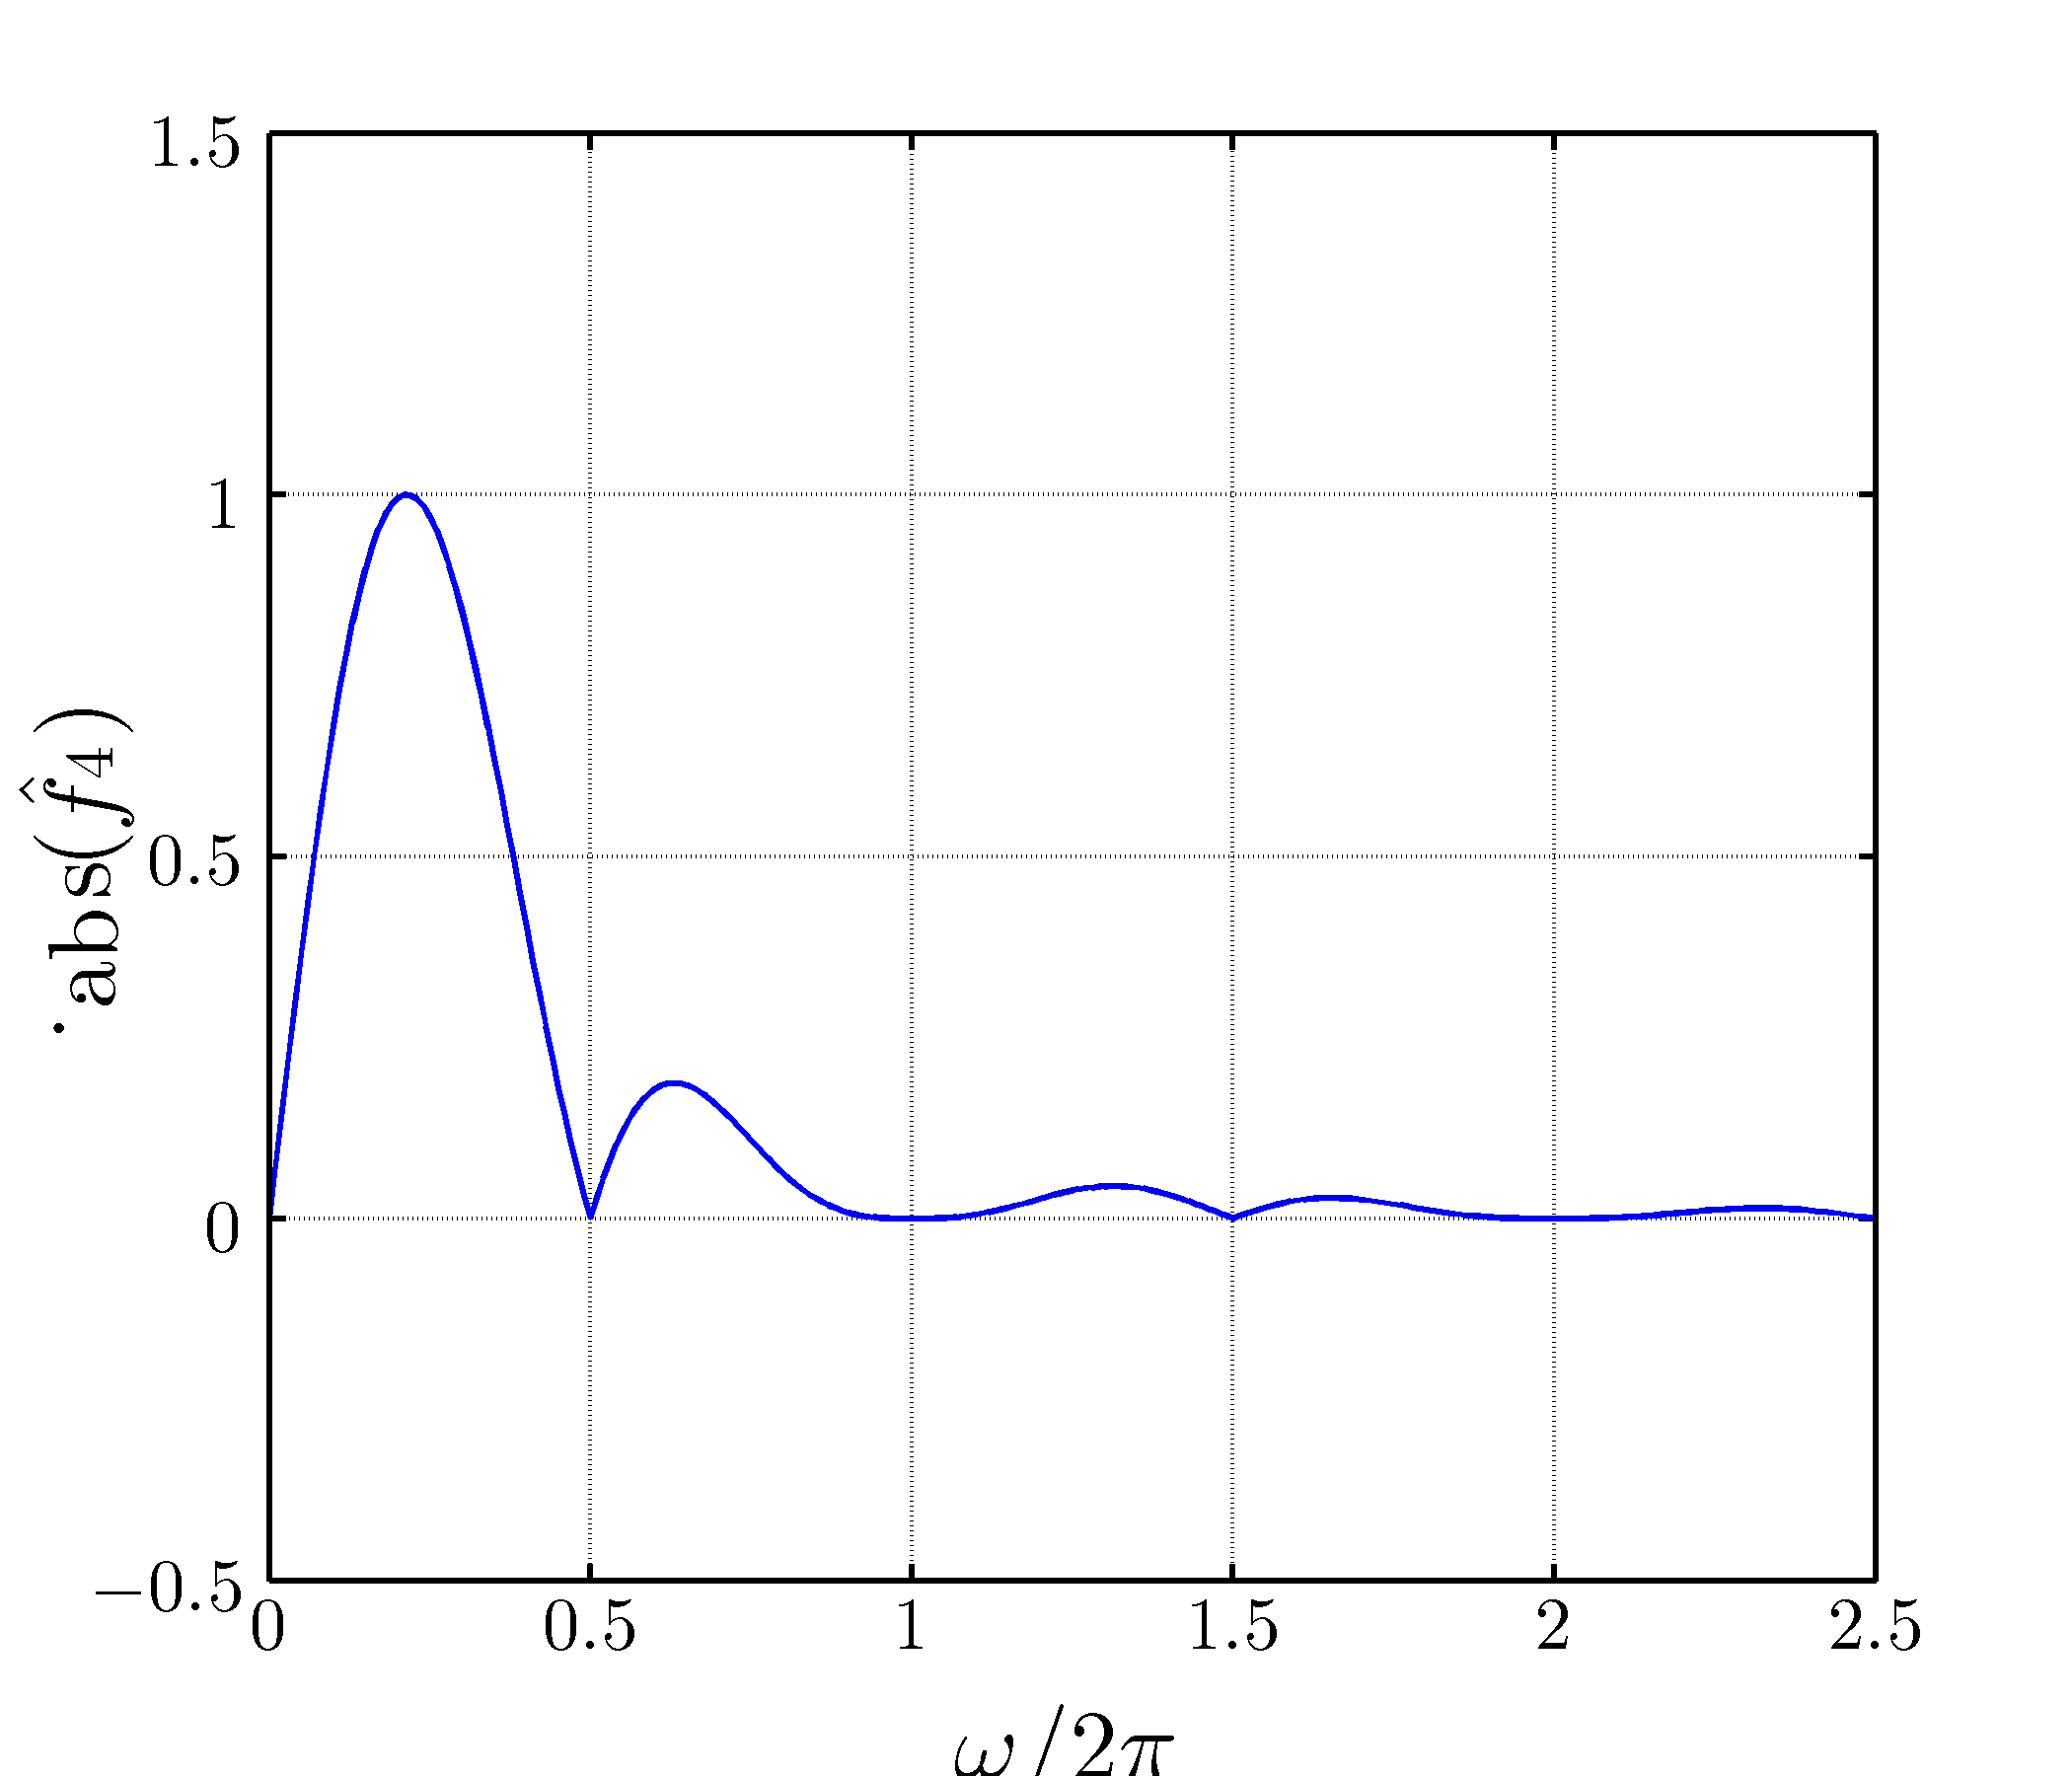
\includegraphics[width=0.45\textwidth]{./laboratorio_4/problema01_F4.png}
        \end{center}
      \end{figure}

      \begin{listing}[H]
        \caption{Script para obtener las \emph{figs. \ref{script01Afigure}, \ref{script01Bfigure}, \ref{script01Cfigure}} y \emph{\ref{script01Dfigure}.}}
        \label{script01G}
        \inputminted{matlab}{./laboratorio_4/problema01.m}
      \end{listing}\vspace{-1.0em}

  \newpage
  \subsection*{Problema 2}
    \floatsetup[figure]{
      capposition=top,
      style=plain,
    }

    \noindent Hallar la transformada de Fourier de $x\left(t\right)$ y graficar en Matlab:

      \begin{figure}[H]
        \begin{center}
          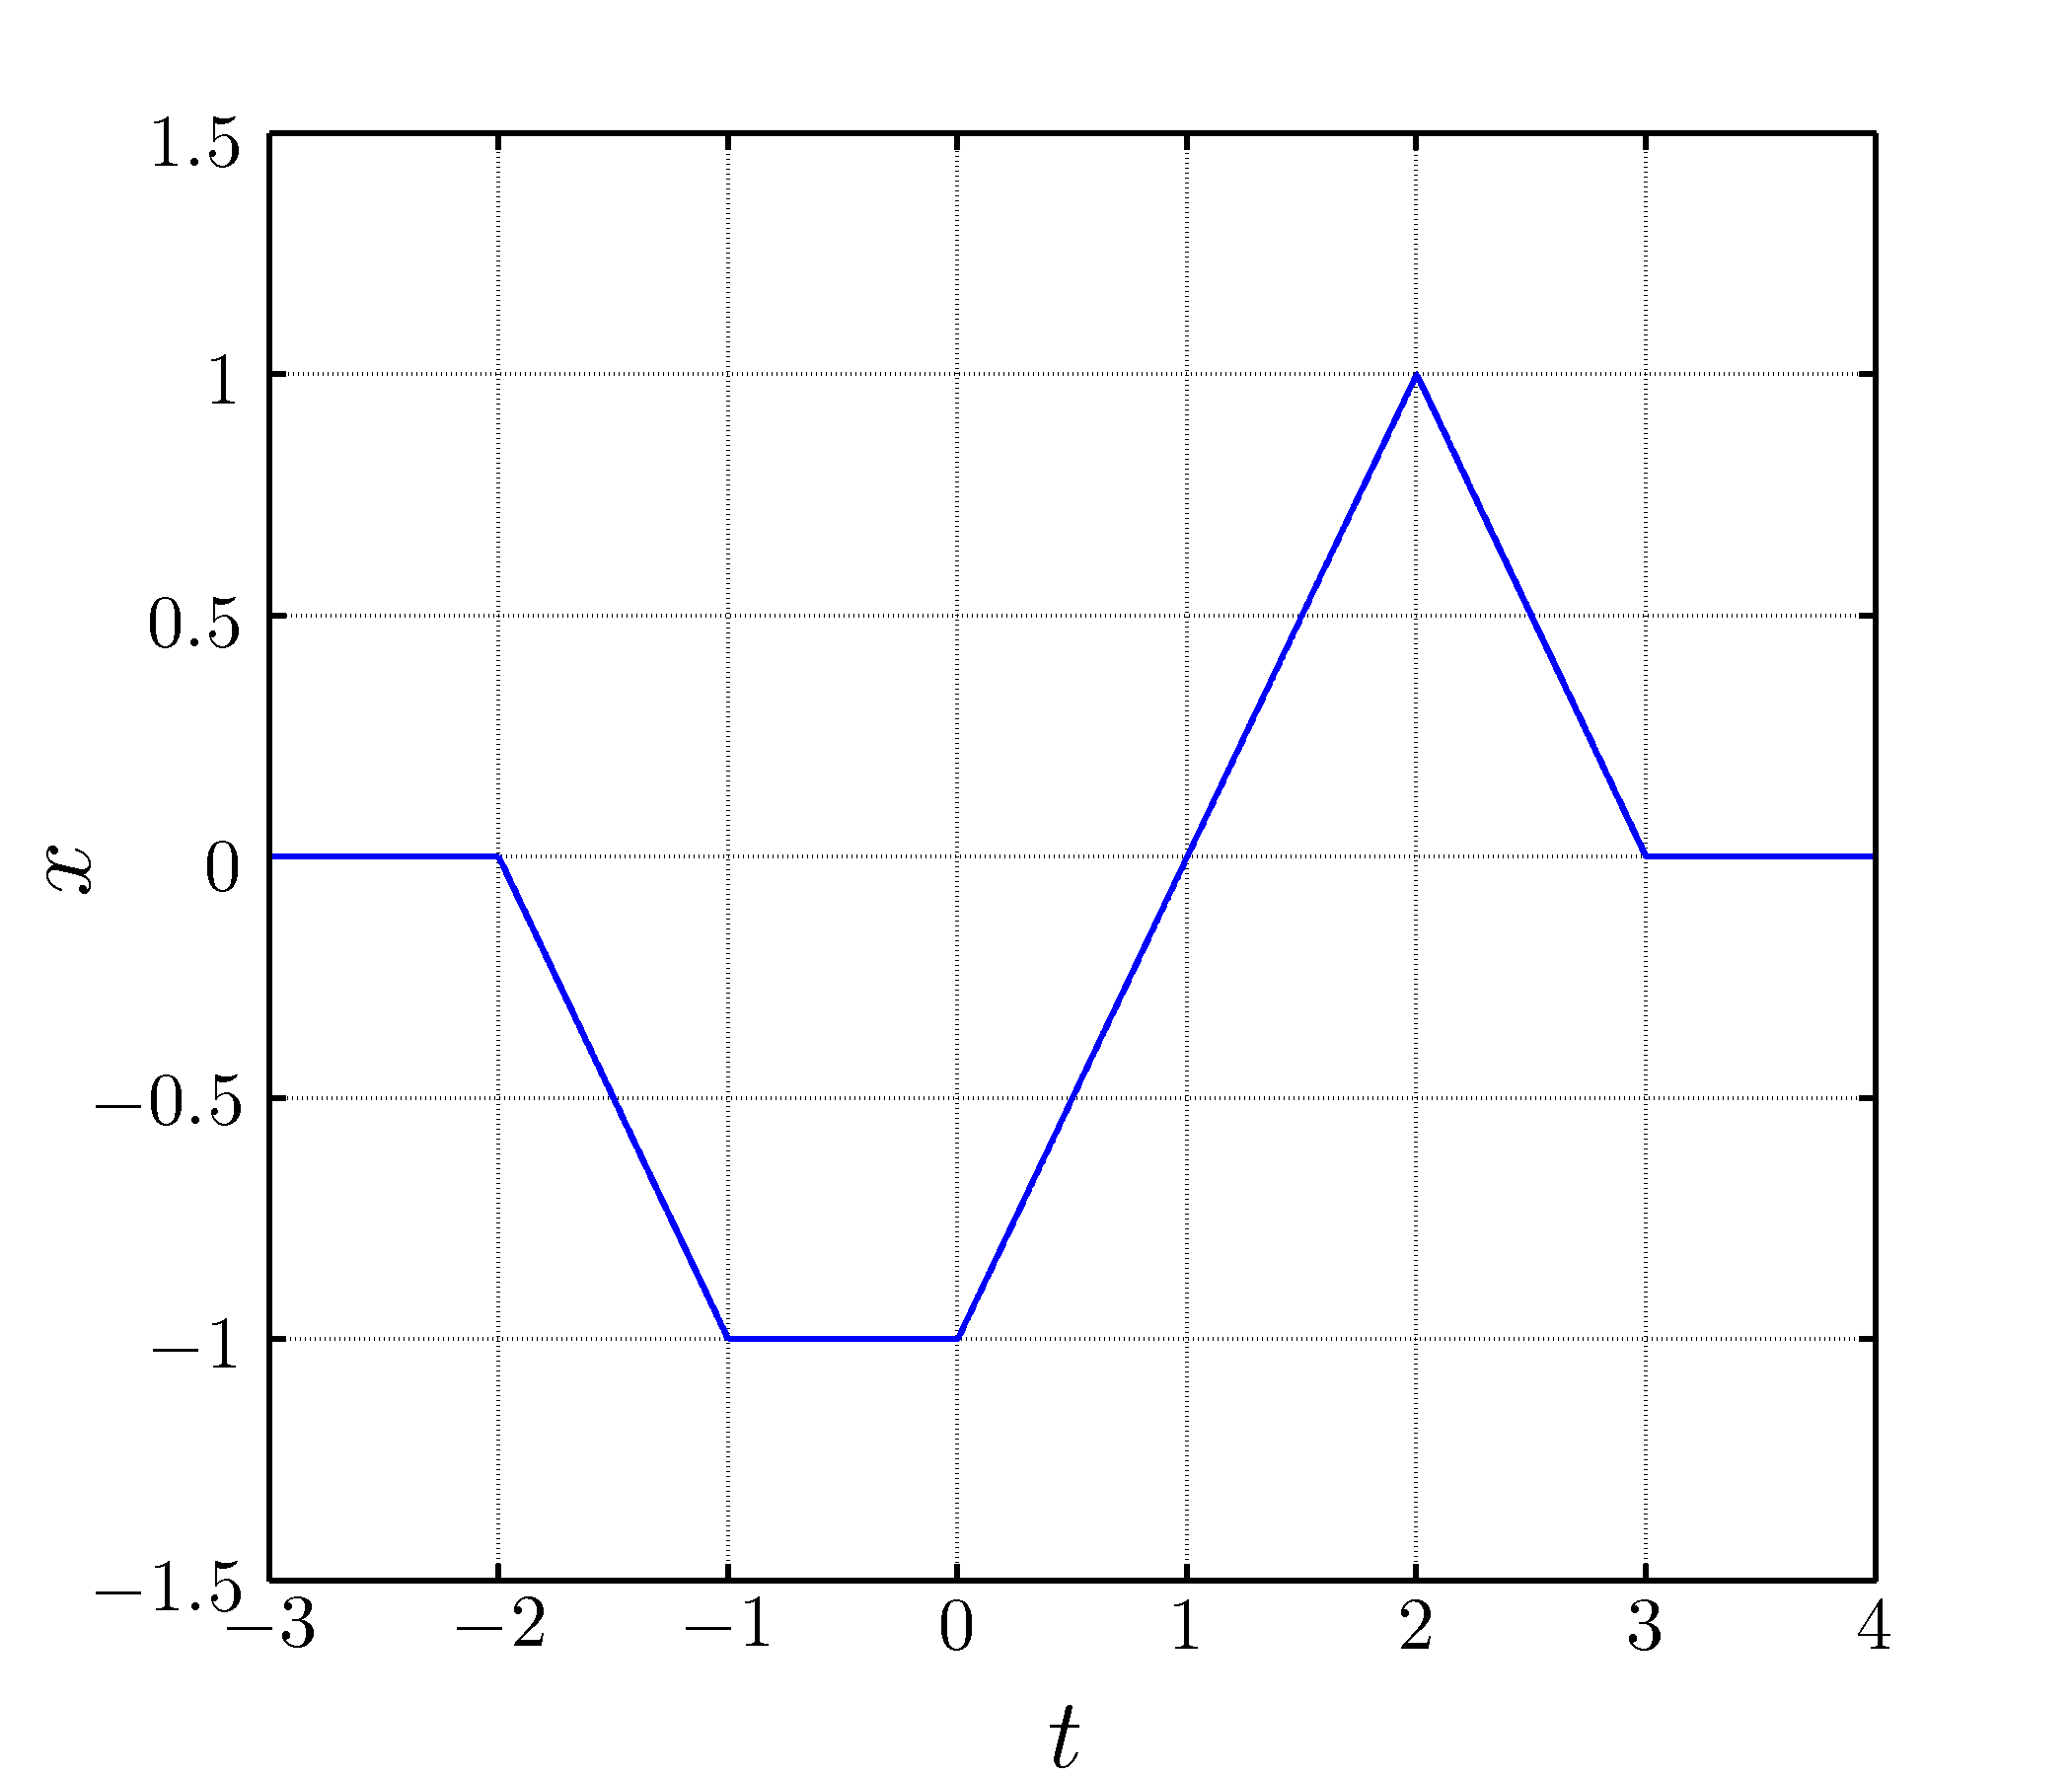
\includegraphics[width=0.45\textwidth]{./laboratorio_4/problema02_x.png}
        \end{center}
      \end{figure}

    \noindent Si $x\left(t\right)$ pasa a través del bloque de la figura,
      calcule la transformada de Fourier de $y\left(t\right)$.

      \begin{figure}[H]
        \begin{center}
          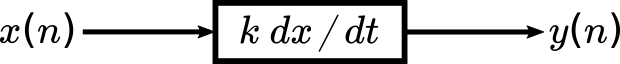
\includegraphics[width=0.45\textwidth]{./laboratorio_4/problema02_diagram.png}
        \end{center}
      \end{figure}\vspace{-1.5em}

    \subsubsection*{Solución}
      \floatsetup[figure]{
        capposition=top,
        style=ruled,
      }

      \noindent La función $x\left(t\right)$ se puede modelar empleando la función triángulo como

        \begin{equation*}
         x\left(t\right) = - \Lambda\left(\frac{1}{2}t + \frac{1}{2}\right)
                           - \Lambda\left(\frac{1}{2}t \right)
                           + \Lambda\left(\frac{1}{2}t - 1\right).
        \end{equation*}

      \noindent Así, la transformada de fourier vendrá dada por:

        \begin{equation*}
          \begin{split}
            \widehat{f}\left(\omega\right) & = - \mathcal{F}\left(\Lambda,\left.\frac{t}{2} + \frac{1}{2} \right|\omega\right) - \mathcal{F}\left(\Lambda,\left.\frac{t}{2}\right|\omega\right) + \mathcal{F}\left(\Lambda,\left.\frac{t}{2}\right|\omega\right) \\
                                           & = - 2 \mathcal{F}\left(\Lambda,t + 1 |2 \omega\right) - 2 \mathcal{F}\left(\Lambda,t|2 \omega\right) + 2 \mathcal{F}\left(\Lambda,\left.t - 2\right| 2 \omega\right) \\
                                           & = - 2 \exp\left(i \omega\right) \mathcal{F}\left(\Lambda,t |2 \omega\right) - 2 \mathcal{F}\left(\Lambda,t|2 \omega\right) + 2 \exp\left(- 2 i \omega\right) \mathcal{F}\left(\Lambda,t| 2 \omega\right) \\
                                           & = - \exp\left(i \omega\right) \mathrm{sinc}^{2}\left(\frac{\omega}{2}\right) - \mathrm{sinc}^{2}\left(\frac{\omega}{2}\right) + \exp\left(- 2 i \omega\right) \mathrm{sinc}^{2}\left(\frac{\omega}{2}\right) \\
                                           & = \left( - \exp\left(i \omega\right) - 1 + \exp\left(- 2 i \omega\right) \right) \mathrm{sinc}^{2}\left(\frac{\omega}{2}\right)
          \end{split}
        \end{equation*}

      \noindent En \textsc{Matlab} implementamos la función $x\left(t\right)$
        en términos de la función triángulo tal como muestra el \emph{script
        \ref{script02A}} y calculamos su espectro de potencia según el
        \emph{script \ref{script02B}} para obtner la \emph{figura
        \ref{script02Bfigure}}

        \begin{listing}[H]
          \caption{Función $x\left(t\right)$.}
          \label{script02A}
          \inputminted{matlab}{./laboratorio_4/p2_x.m}
        \end{listing}

        \begin{listing}[H]
          \caption{Función $x\left(t\right)$.}
          \label{script02B}
          \inputminted{matlab}{./laboratorio_4/problema02.m}
        \end{listing}

      \begin{figure}[H]
          \caption{Función $x\left(t\right)$ y espectro su espectro de potencia normalizado.}
          \label{script02Afigure}
          \begin{center}
              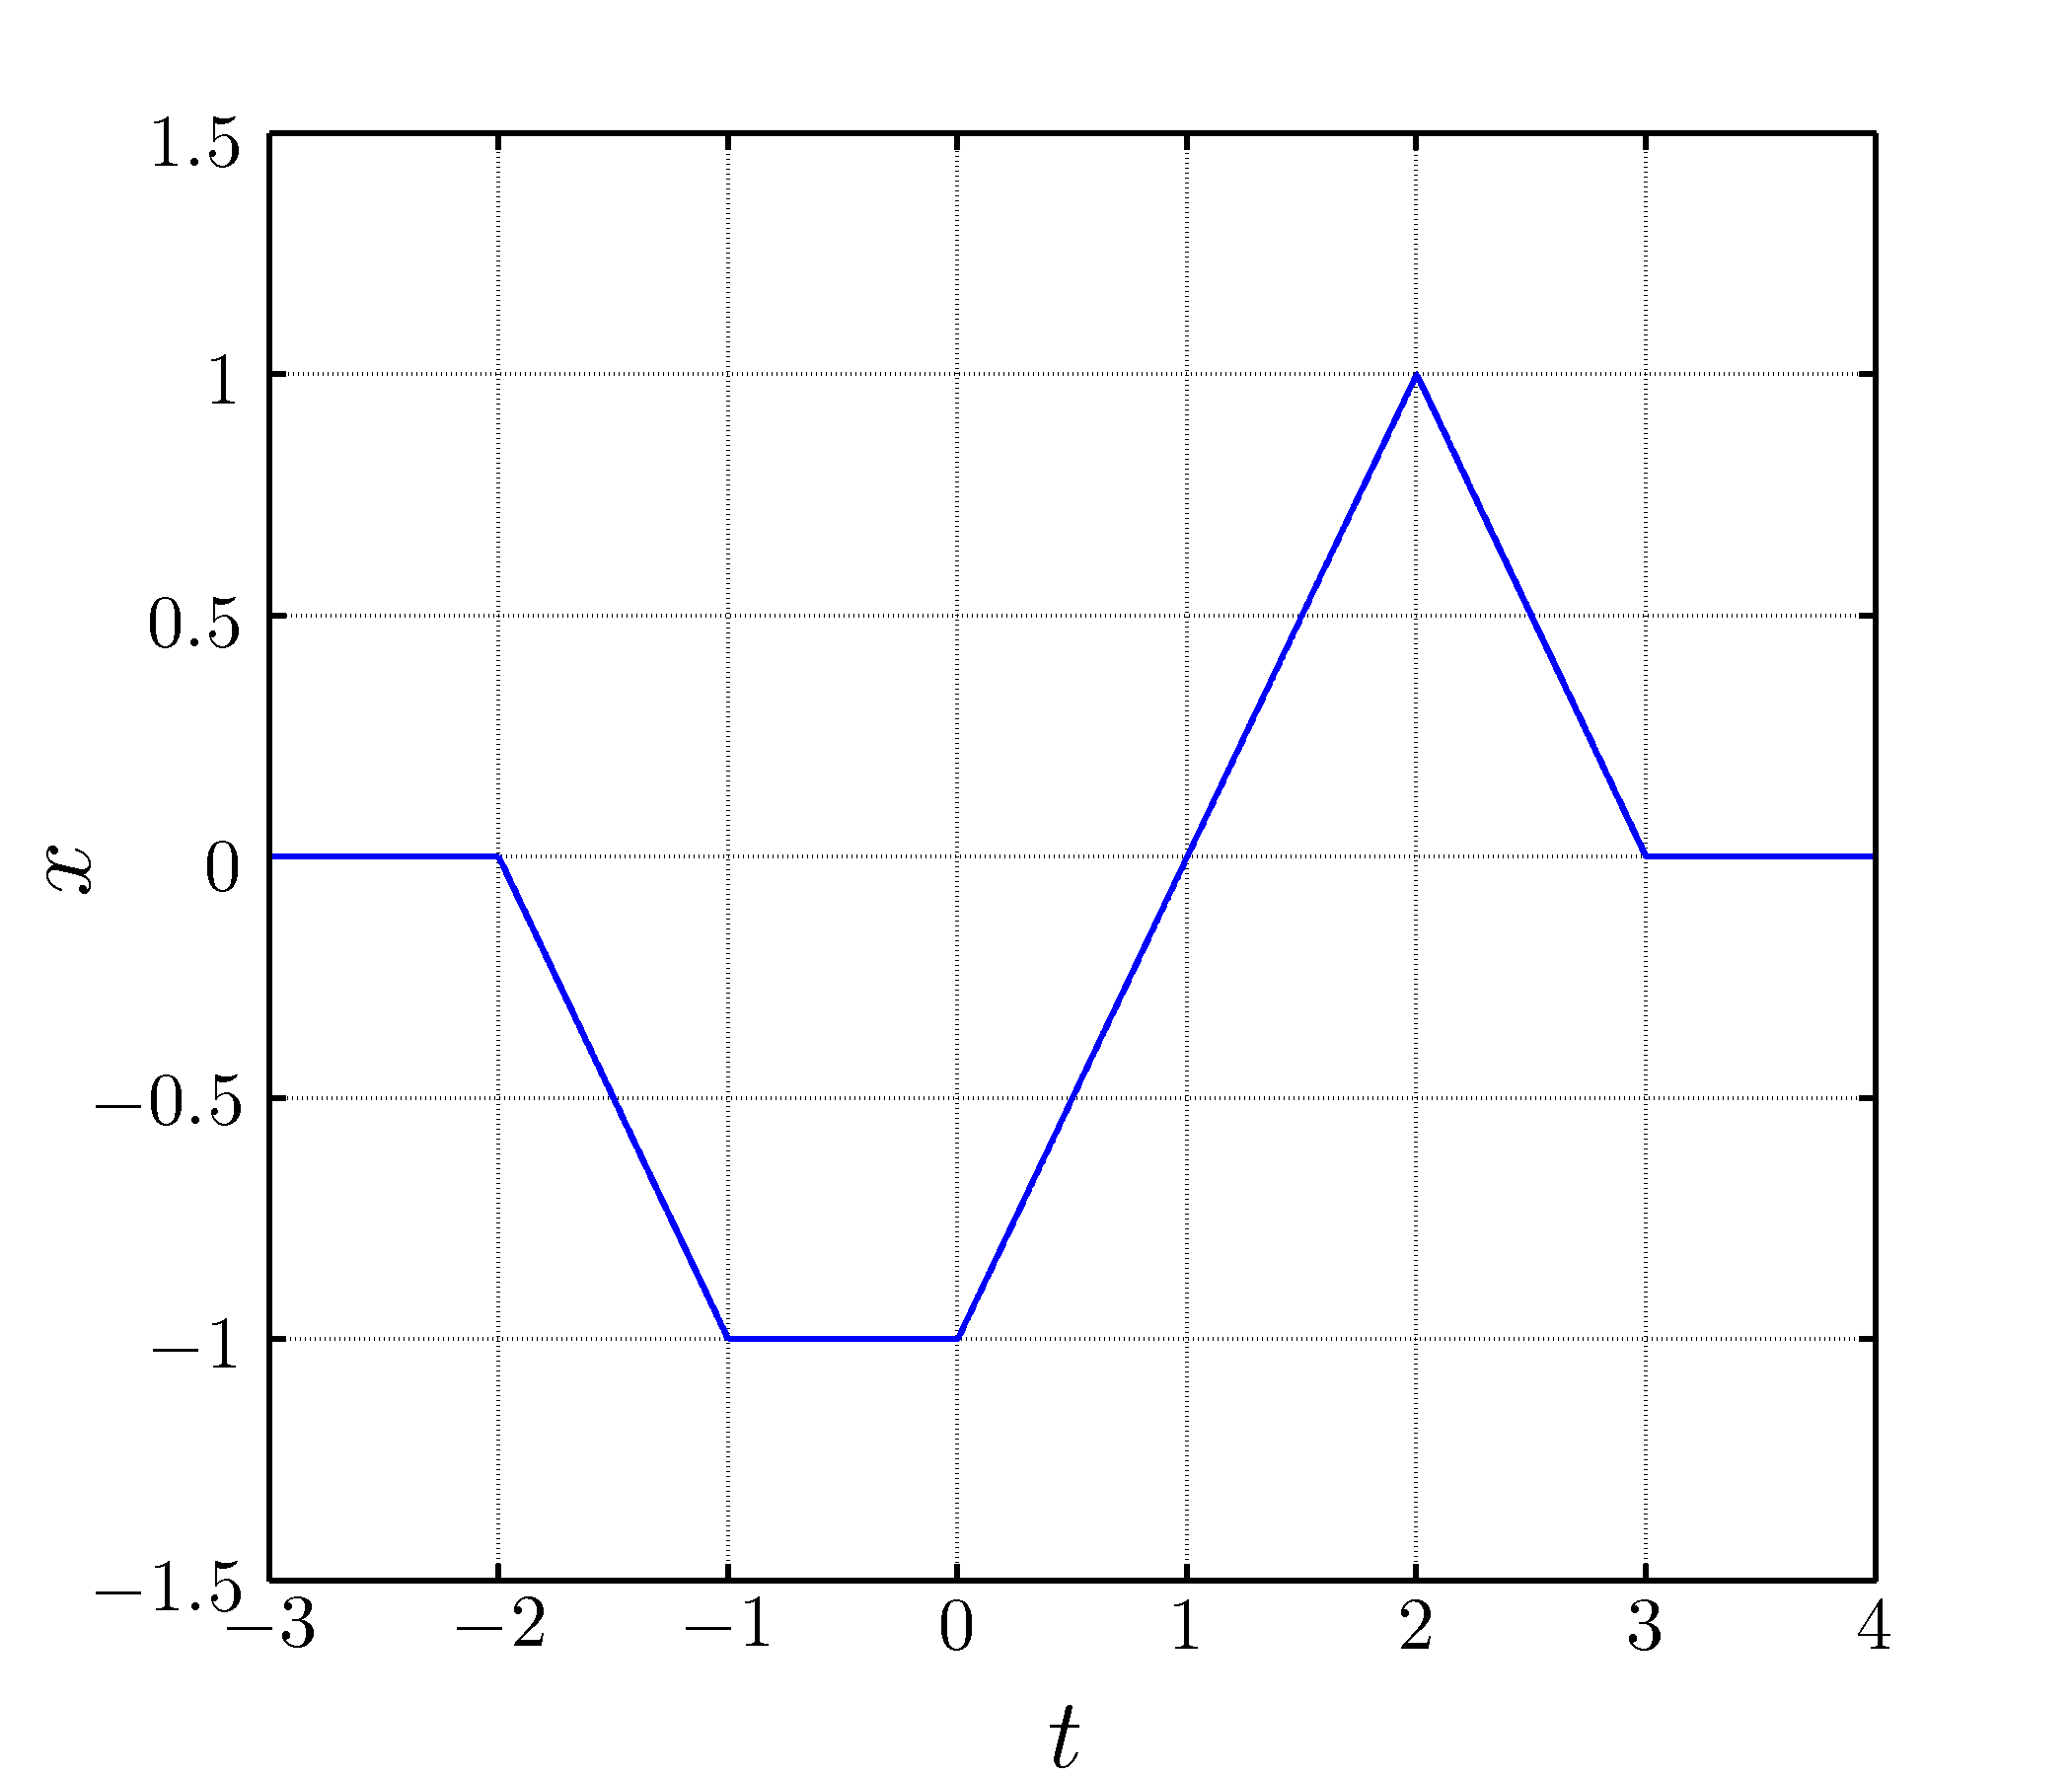
\includegraphics[width=0.45\textwidth]{./laboratorio_4/problema02_x.png}
              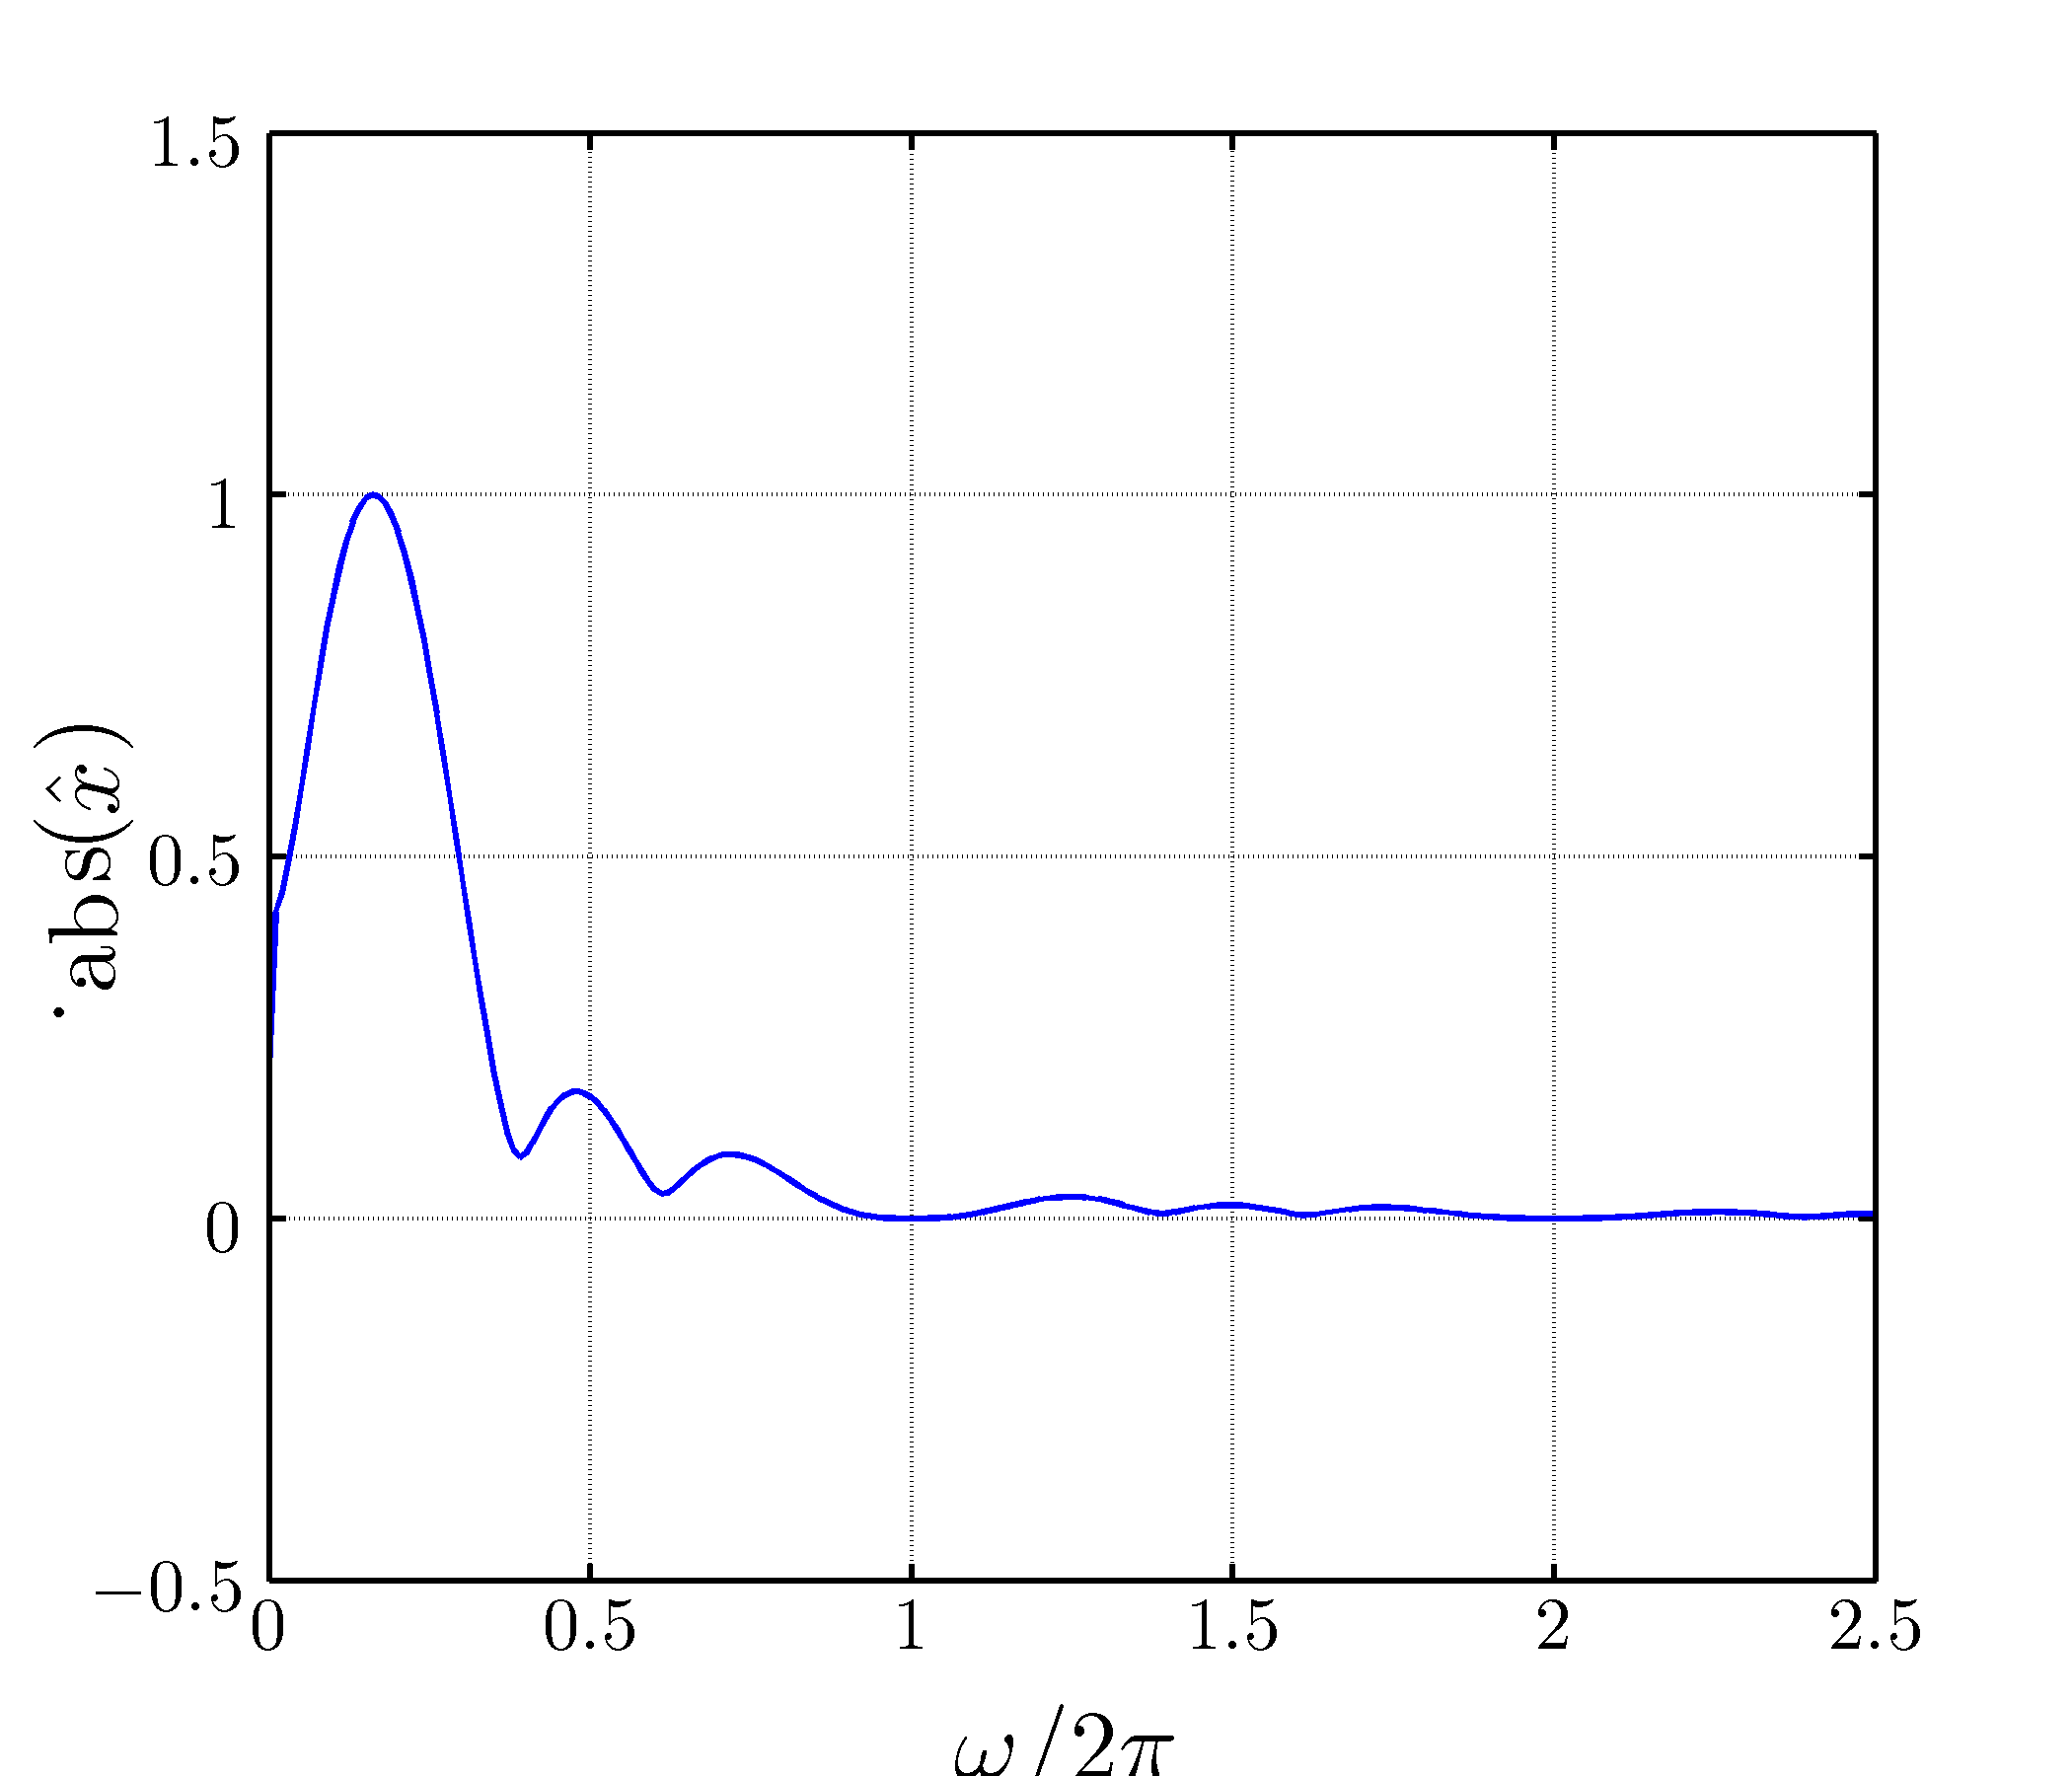
\includegraphics[width=0.45\textwidth]{./laboratorio_4/problema02_X.png}
          \end{center}
      \end{figure}

  \newpage
  \subsection*{Problema 3}
    \noindent Calcular la convolución entre los siguientes pares de señales:
    \begin{enumerate}[label=\alph*)]
      \item $x\left(n\right) = \left(\frac{1}{2}\right)^n u\left(n-4\right)$ y $h\left(n\right) = 4^n u\left(2-n\right)$
      \item $x\left(n\right) = u\left(-n\right) - u\left(-n-2\right)$ y $h\left(n\right) = u\left(n-1\right) - u\left(n-4\right)$
      \item $x\left(n\right) = u\left(n\right)$ y $h\left(n\right) = \left(\frac{1}{2}\right)^{-n} u\left(-n\right)$
      \item $x\left(t\right) = \exp\left(-at\right) u(t)$ y $h(t) = exp(-at) u(t)$
    \end{enumerate}

    \noindent Donde $u\left(n\right)$ es la función escalón unitario.

    \subsubsection*{Solución}
      \begin{enumerate}[label=\alph*)]
        \item $x\left(n\right) = \left(\frac{1}{2}\right)^n u\left(n-4\right)$ y $h\left(n\right) = 4^n u\left(2-n\right)$

          \begin{equation*}
            \begin{split}
              y\left(m\right) & = x\left(n\right) * h\left(n\right) \\
                              & = \sum_{n=-\infty}^{\infty} x\left(n\right)h\left(m-n\right) \\
                              & = \sum_{n=-\infty}^{\infty} \left(\frac{1}{2}\right)^n u\left(n-4\right)4^{m-n} u\left(2-m+n\right) \\
                              & = \sum_{n=-\infty}^{\infty} 2^{2m-3n} u\left(n-4\right) u\left(n+2-m\right) \\
            \end{split}
          \end{equation*}

          \noindent Cuando $m<6$:

          \begin{equation*}
            \begin{split}
              y\left(m\right) & = \sum_{n=-\infty}^{\infty} 2^{2m-3n} u\left(n-4\right) u\left(n+2-m\right) \\
                              & = \sum_{n=-\infty}^{\infty} 2^{2m-3n} u\left(n-4\right) \\
                              & = \sum_{n=4}^{\infty} 2^{2m-3n} \\
                              & = \sum_{n=0}^{\infty} 2^{2m-3\left(n+4\right)} \\
                              & = \sum_{n=0}^{\infty} 2^{2m-3n-12} \\
                              & = 2^{2m-12} \sum_{n=0}^{\infty} \left(2^{-3}\right)^{n} \\
                              & = 2^{2m-12} \sum_{n=0}^{\infty} \left(\frac{1}{8}\right)^{n} \\
                              & = 2^{2m-12} \left(\frac{1}{1-\frac{1}{8}}\right) \\
                              & = \frac{2^{2m-9}}{7}
            \end{split}
          \end{equation*}
          \vfill
          \newpage

          \noindent Cuando $m \geq 6$:

          \begin{equation*}
            \begin{split}
              y\left(m\right) & = \sum_{n=-\infty}^{\infty} 2^{2m-3n} u\left(n-4\right) u\left(n+2-m\right) \\
                              & = \sum_{n=-\infty}^{\infty} 2^{2m-3n} u\left(n+2-m\right) \\
                              & = \sum_{n=m-2}^{\infty} 2^{2m-3n} \\
                              & = \sum_{n=0}^{\infty} 2^{2m-3\left(n+m-2\right)} \\
                              & = \sum_{n=0}^{\infty} 2^{6-m-3n} \\
                              & = 2^{6-m} \sum_{n=0}^{\infty} \left(2^{-3}\right)^{n} \\
                              & = 2^{6-m} \sum_{n=0}^{\infty} \left(\frac{1}{8}\right)^{n} \\
                              & = 2^{6-m} \left(\frac{1}{1-\frac{1}{8}}\right) \\
                              & = \frac{2^{9-m}}{7}
            \end{split}
          \end{equation*}

          \noindent Finalmente

          \begin{equation*}
            y\left(m\right) = \left\{
              \begin{array}{lcl}
                \displaystyle{\frac{2^{2m-9}}{7}} &;& n < 6 \\ [1em]
                \displaystyle{\frac{2^{9-m}}{7}}  &;& n \geq 6
              \end{array}
            \right.
          \end{equation*}

        \item $x\left(n\right) = u\left(-n\right) - u\left(-n-2\right)$ y $h\left(n\right) = u\left(n-1\right) - u\left(n-4\right)$
          \begin{equation*}
            \begin{split}
              y\left(m\right) & = x\left(n\right) * h\left(n\right) \\
                              & = \sum_{n=-\infty}^{\infty} x\left(n\right)h\left(m-n\right) \\
                              & = \sum_{n=-\infty}^{\infty} \left[u\left(-n\right) - u\left(-n-2\right)\right]
                                                            \left[u\left(m-n-1\right) - u\left(m-n-4\right)\right] \\
                              & = \sum_{n=-\infty}^{\infty} u\left(-n\right)u\left(m-n-1\right) - \sum_{n=-\infty}^{\infty} u\left(-n-2\right)u\left(m-n-1\right) - \\
                              & \phantom{=}\ \sum_{n=-\infty}^{\infty} u\left(-n\right)u\left(m-n-4\right) + \sum_{n=-\infty}^{\infty} u\left(-n-2\right)u\left(m-n-4\right)
            \end{split}
          \end{equation*}
          \vfill
          \newpage

          \noindent Cuando $m<0$:

          \begin{equation*}
            \begin{split}
              y\left(m\right) & = \sum_{n=-\infty}^{m-1} 1 -
                                  \sum_{n=-\infty}^{m-1} 1 -
                                  \sum_{n=-\infty}^{m-4} 1 +
                                  \sum_{n=-\infty}^{m-4} 1 \\
                              & = 0
            \end{split}
          \end{equation*}

          \noindent Cuando $m=0$:

          \begin{equation*}
            \begin{split}
              y\left(m\right) & = \sum_{n=-\infty}^{-1} 1 -
                                  \sum_{n=-\infty}^{-2} 1 -
                                  \sum_{n=-\infty}^{-3} 1 +
                                  \sum_{n=-\infty}^{-3} 1 \\
                              & = 1
            \end{split}
          \end{equation*}

          \noindent Cuando $0<m \wedge m<3$:

          \begin{equation*}
            \begin{split}
              y\left(m\right) & = \sum_{n=-\infty}^{0} 1 -
                                  \sum_{n=-\infty}^{-2} 1 -
                                  \sum_{n=-\infty}^{-2} 1 +
                                  \sum_{n=-\infty}^{-2} 1 \\
                              & = 2
            \end{split}
          \end{equation*}

          \noindent Cuando $m=3$:

          \begin{equation*}
            \begin{split}
              y\left(m\right) & = \sum_{n=-\infty}^{0} 1 -
                                  \sum_{n=-\infty}^{-2} 1 -
                                  \sum_{n=-\infty}^{-1} 1 +
                                  \sum_{n=-\infty}^{-2} 1 \\
                              & = 1
            \end{split}
          \end{equation*}

          \noindent Cuando $m>3$:

          \begin{equation*}
            \begin{split}
              y\left(m\right) & = \sum_{n=-\infty}^{0} 1 -
                                  \sum_{n=-\infty}^{-1} 1 -
                                  \sum_{n=-\infty}^{0} 1 +
                                  \sum_{n=-\infty}^{-1} 1 \\
                              & = 0
            \end{split}
          \end{equation*}

          \noindent Finalmente

          \begin{equation*}
            y\left(m\right) = \left\{
              \begin{array}{lcl}
                0 &;& m < 0  \vee  3 < m \\ [1em]
                1 &;& m = 0  \vee  m = 3 \\ [1em]
                2 &;& 0 < m \wedge m < 3
              \end{array}
            \right.
          \end{equation*}
          \vfill
          \newpage

        \item $x\left(n\right) = u\left(n\right)$ y $h\left(n\right) = \left(\frac{1}{2}\right)^{-n} u\left(-n\right)$

          \begin{equation*}
            \begin{split}
              y\left(m\right) & = x\left(n\right) * h\left(n\right) \\
                              & = \sum_{n=-\infty}^{\infty} x\left(n\right)h\left(m-n\right) \\
                              & = \sum_{n=-\infty}^{\infty} u\left(n\right) \left(\frac{1}{2}\right)^{n-m} u\left(n-m\right) \\
                              & = \sum_{n=-\infty}^{\infty} \left(\frac{1}{2}\right)^{n-m} u\left(n\right) u\left(n-m\right)
            \end{split}
          \end{equation*}

          \noindent Cuando $m < 0$:

          \begin{equation*}
            \begin{split}
              y\left(m\right) & = \sum_{n=-\infty}^{\infty} \left(\frac{1}{2}\right)^{n-m} u\left(n\right) u\left(n-m\right) \\
                              & = \sum_{n=0}^{\infty} \left(\frac{1}{2}\right)^{n-m} \\
                              & = 2^{m} \sum_{n=0}^{\infty} \left(\frac{1}{2}\right)^{n} \\
                              & = 2^{1+m}
            \end{split}
          \end{equation*}

          \noindent Cuando $0 \leq m$:

          \begin{equation*}
            \begin{split}
              y\left(m\right) & = \sum_{n=-\infty}^{\infty} \left(\frac{1}{2}\right)^{n-m} u\left(n\right) u\left(n-m\right) \\
                              & = \sum_{n=0}^{\infty} \left(\frac{1}{2}\right)^{n-m} \\
                              & = 2^{m} \sum_{n=0}^{\infty} \left(\frac{1}{2}\right)^{n} \\
                              & = 2^{1+m}
            \end{split}
          \end{equation*}

        \item $x\left(t\right) = \exp\left(-at\right) u(t)$ y $h(t) = \exp\left(-at\right) u(t)$

          \begin{equation*}
            \begin{split}
              y\left(\tau\right) & = x\left(t\right) * h\left(t\right) \\
                                 & = \int_{-\infty}^{\infty} x\left(t\right)h\left(\tau-t\right)dt \\
                                 & = \int_{-\infty}^{\infty} \exp\left(-at\right) u(t) \exp\left(-a\tau + at\right) u(t-\tau) dt\\
                                 & = \int_{0}^{\tau} \exp\left(-a\tau\right) dt \\
                                 & = \exp\left(-a\tau\right) \tau
            \end{split}
          \end{equation*}

      \end{enumerate}

  \newpage
  \subsection*{Problema 4}
    \noindent Para el diagrama de bloques mostrado
    \begin{figure}[H]
      \begin{center}
        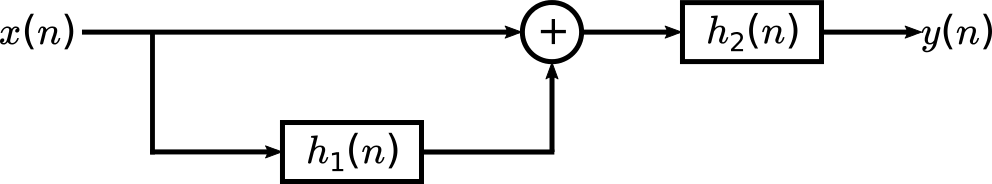
\includegraphics[width=0.7\textwidth]{./laboratorio_3/problema04_diagram.png}
      \end{center}
    \end{figure}

    \noindent Donde

    $$h_1\left(n\right) = \beta\delta\left(n-1\right)$$

    \noindent y

    $$h_2\left(n\right) = \exp\left(\alpha\right)\delta\left(n\right)$$

    \begin{enumerate}[label=\alph*)]
      \item Escribir la ecuación en diferencias que relaciona la entrada con la salida
      \item Hallar $\alpha$ y $\beta$, de tal forma que la salida sea el promedio entre la entrada en el instante $n$ y
      la entrada en el instante $n-1$.
    \end{enumerate}

    \subsubsection*{Solución}
      \begin{enumerate}[label=\alph*)]
        \item La ecuación en diferencias se obtiene de calcular
          $$ y\left(n\right) = \left[\left(x + x*h_1\right)*h_2\right]\left(n\right) $$

          \noindent Resolviendo $\left[x*h_1\right]\left(n\right)$, tenemos

          \begin{equation*}
            \begin{split}
              y_1\left(n\right) & = x(m)*h_1(m) \\
                                & = \sum_{m=-\infty}^{\infty} x\left(m\right)h_1\left(n-m\right) \\
                                & = \sum_{m=-\infty}^{\infty} x\left(m\right)\beta\delta\left(n-m-1\right) \\
                                & = \beta x\left(n-1\right)
            \end{split}
          \end{equation*}

          \noindent Haciendo $y_2\left(n\right)=y_1\left(n\right) + x\left(n\right)$, calculamos $\left[y_2*h_2\right]\left(n\right)$ como

          \begin{equation*}
            \begin{split}
              y\left(n\right) & = y_2(m)*h_2(m) \\
                              & = \sum_{m=-\infty}^{\infty} y_2(m)h_2\left(n-m\right) \\
                              & = \sum_{m=-\infty}^{\infty} \left[y_1\left(m\right) + x\left(m\right)\right]\exp\left(\alpha\right)\delta\left(n-m\right) \\
                              & = \sum_{m=-\infty}^{\infty} \left[\beta x\left(m-1\right) + x\left(m\right)\right]\exp\left(\alpha\right)\delta\left(n-m\right) \\
                              & = \left[\beta x\left(n-1\right) + x\left(n\right)\right]\exp\left(\alpha\right)
            \end{split}
          \end{equation*}

          \noindent De modo que la ecuación en diferencias del sistema queda expresada como

          $$y\left(n\right) = \left[\beta x\left(n-1\right) + x\left(n\right)\right]\exp\left(\alpha\right)$$

        \item Para que la señal de salida sea igual al promedio de los valores de la señal de entrada en el instante $n$
          y en el instante $n-1$ se debe resolver el sistema

          \begin{equation}
            \left\{
              \begin{array}{ccc}
                \exp\left(\alpha\right)      &=&  \displaystyle{\frac{1}{2}} \\[1em]
                \exp\left(\alpha\right)\beta &=&  \displaystyle{\frac{1}{2}}
              \end{array}
            \right.
          \end{equation}

          \noindent De donde resulta

          $$ \alpha = \ln\left(\frac{1}{2}\right) \wedge \beta = 1$$
      \end{enumerate}

  \newpage
  \subsection*{Problema 5}
    \noindent Dada la siguiente ecuación en diferencias
    $$y\left(n\right) = -a y\left(n-1\right) + b x\left(n\right) + c x\left(n-1\right),$$
    realizar una representación en diagrama de bloques.

    \subsubsection*{Solución}
      \noindent Expresando la ecuación en diferencias como:

      $$y\left(n\right) = -a y\left(n\right) * \delta\left(n-1\right) + b x\left(n\right) * \delta\left(n\right) + c x\left(n-1\right) * \delta\left(n-1\right)$$

      \noindent De modo que el diagrama de bloques resultante es

      \begin{figure}[H]
        \begin{center}
          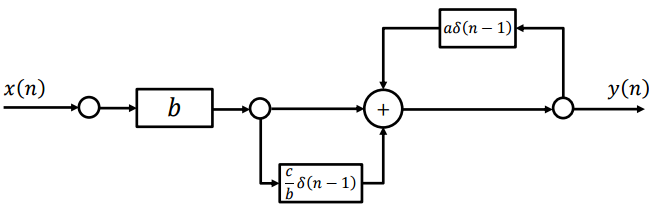
\includegraphics[width=0.7\textwidth]{./laboratorio_3/problema05_diagram.png}
        \end{center}
      \end{figure}

  \newpage
  \subsection*{Problema 6}
    \noindent Realizar en \textsc{Matlab} la convolución del siguiente par de
    señales:

    \begin{enumerate}
        \item $x\left(n\right) = \left(-1\right)^n \left(u\left(n\right) - u\left(-n-8\right)\right)$
        \item $h\left(n\right) = u\left(n\right) - u\left(n-8\right)$
    \end{enumerate}

    \noindent Graficar la señal resultante, $y\left(n\right) = x\left(n\right) * h\left(n\right)$.
    Usar el comando \texttt{stem}.

    \subsubsection*{Solución}
      \noindent xpresamos las funciones $x$ y $h$ en términos de la función escalón unitario $u$.

      \begin{listing}[H]
        \caption{Función escalón unitario}
        \label{script06A}
        \inputminted{matlab}{./laboratorio_3/escalon.m}
      \end{listing}

      \begin{listing}[H]
        \caption{Función $x\left(n\right)$}
        \label{script06B}
        \inputminted{matlab}{./laboratorio_3/p6_X.m}
      \end{listing}

      \begin{listing}[H]
        \caption{Función $h\left(n\right)$}
        \label{script06C}
        \inputminted{matlab}{./laboratorio_3/p6_H.m}
      \end{listing}

    \begin{figure}[H]
      \begin{center}
        \caption{Gráfico de la función $x\left(n\right)$ del \emph{script \ref{script06B}}.}
        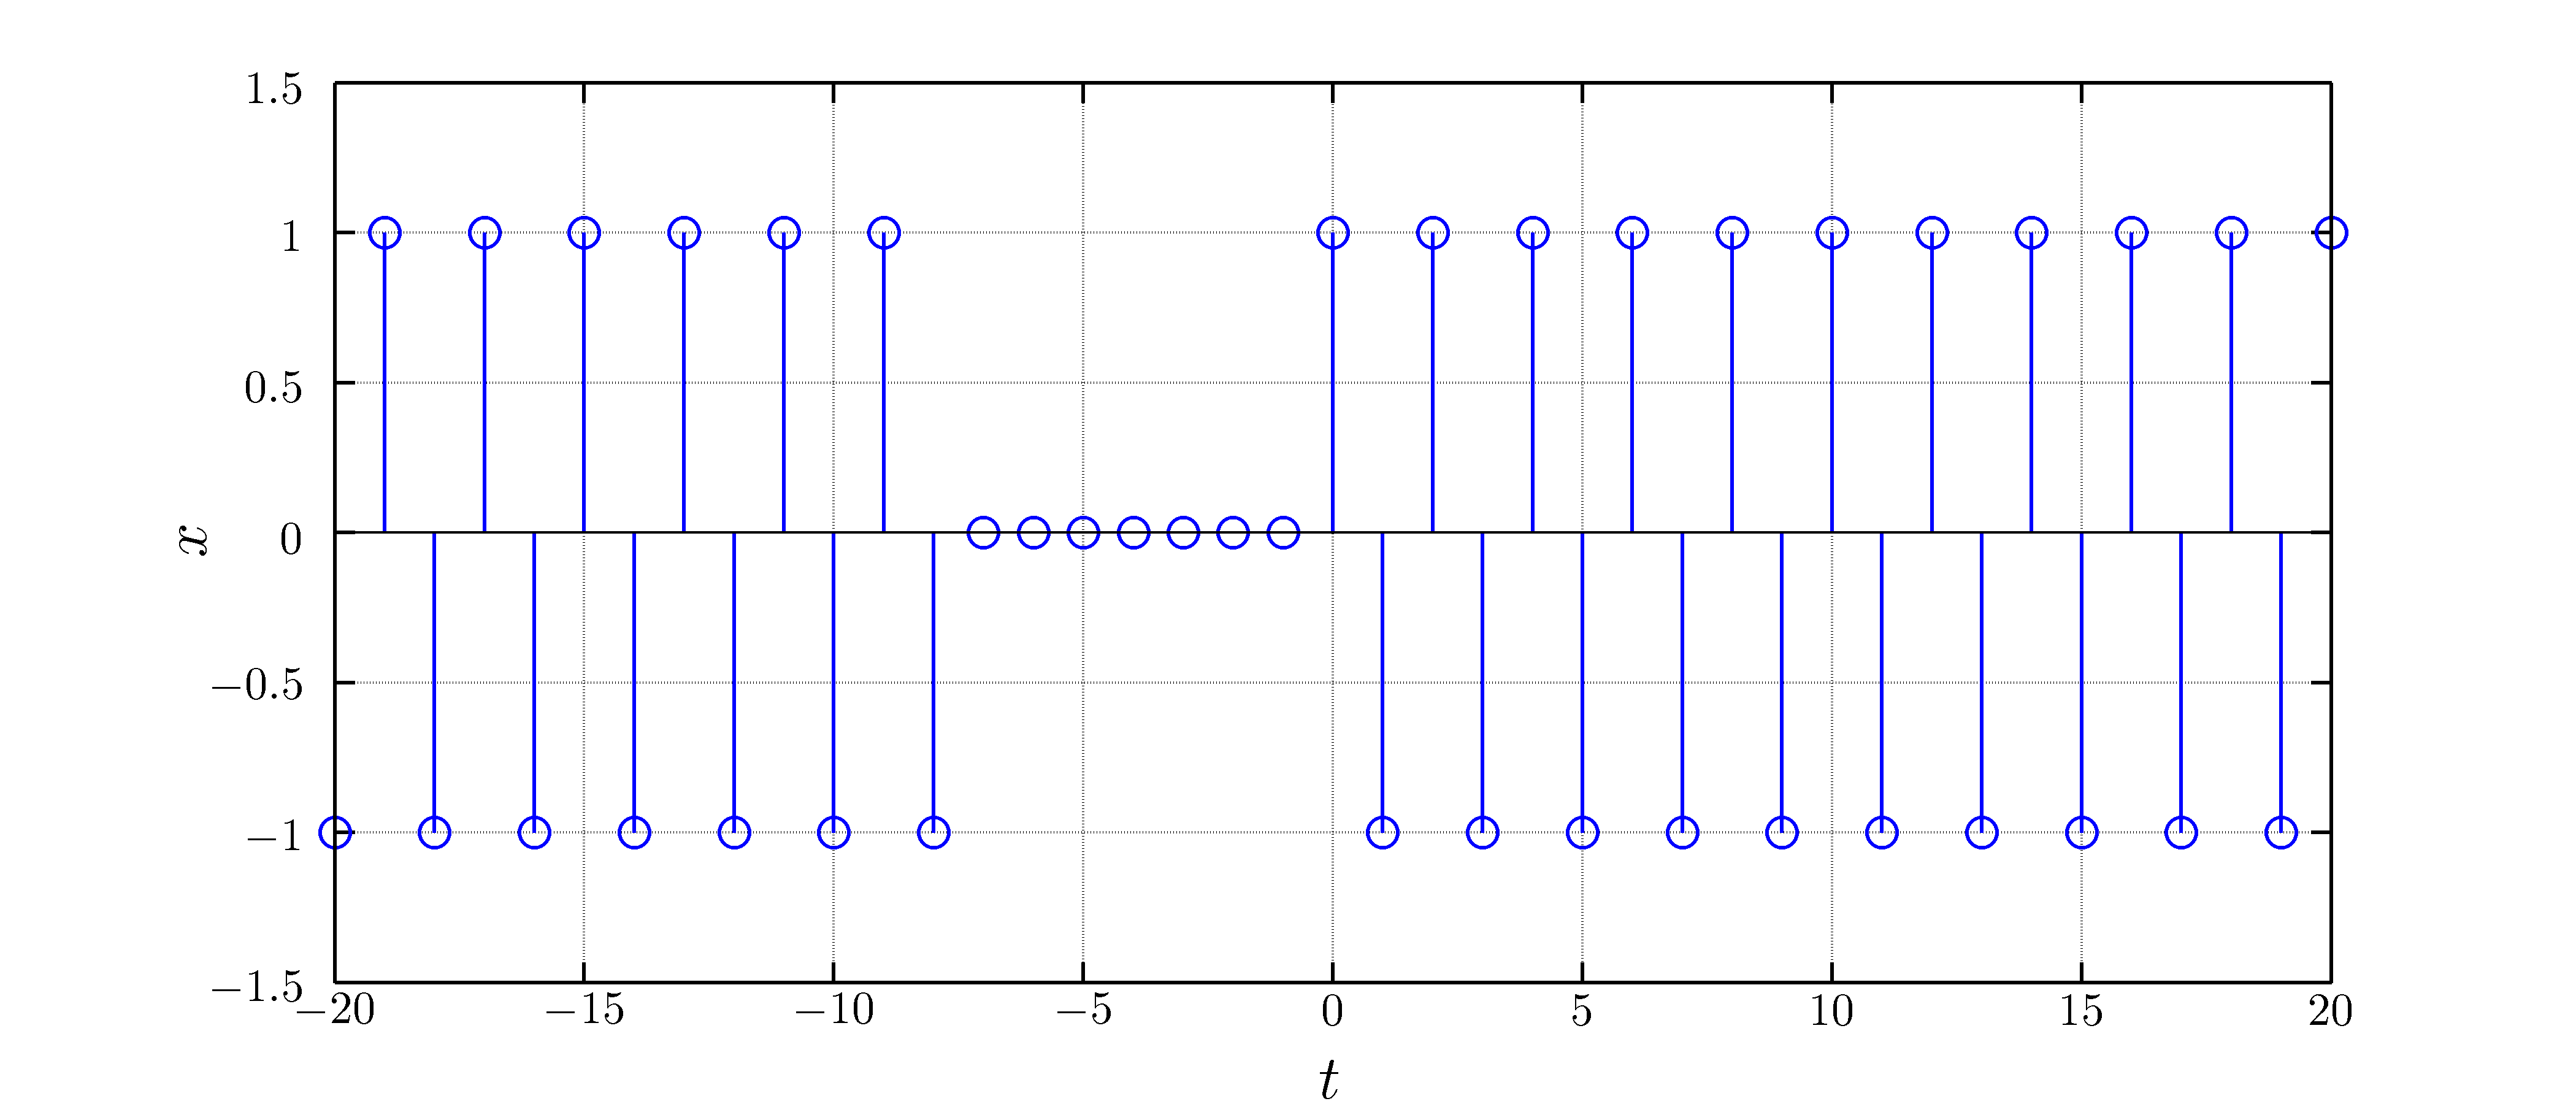
\includegraphics[width=0.90\textwidth]{./laboratorio_3/problema06_X.png}
      \end{center}
    \end{figure}

    \begin{figure}[H]
      \begin{center}
        \caption{Gráfico de la función $x\left(n\right)$ del \emph{script \ref{script06C}}.}
        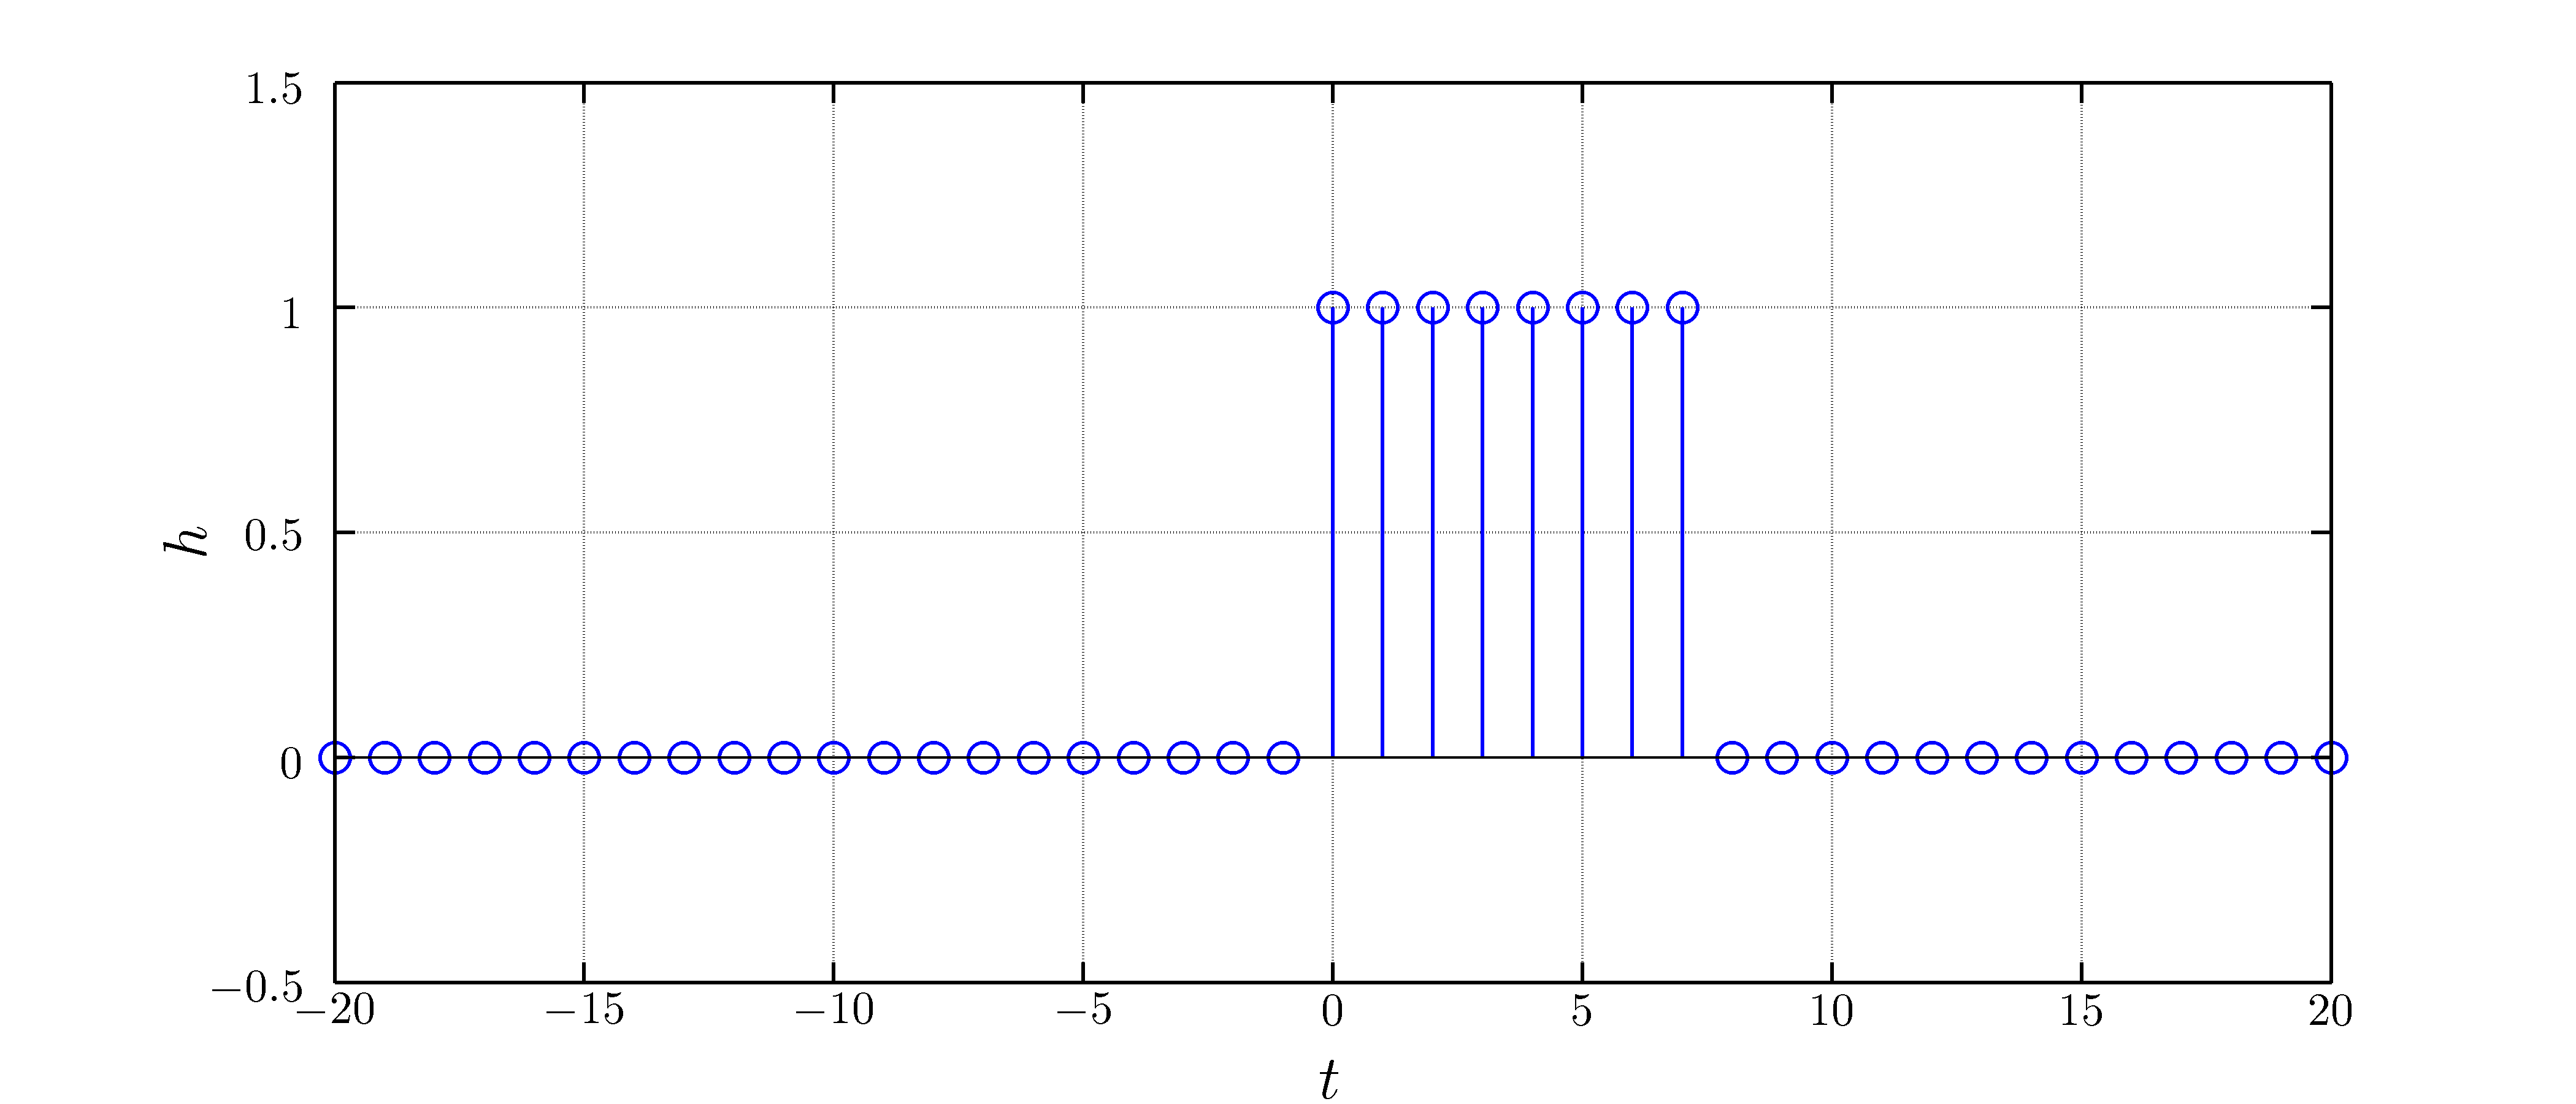
\includegraphics[width=0.90\textwidth]{./laboratorio_3/problema06_H.png}
      \end{center}
    \end{figure}

    \begin{listing}[H]
      \caption{Convlución de las señales $x\left(n\right)$ y $h\left(n\right)$ }
      \label{script06D}
      \inputminted{matlab}{./laboratorio_3/problema06.m}
    \end{listing}

    \begin{figure}[H]
      \begin{center}
        \caption{Gráfico de la función $y\left(n\right) = x\left(n\right) * h\left(n\right)$ del \emph{script \ref{script06D}}.}
        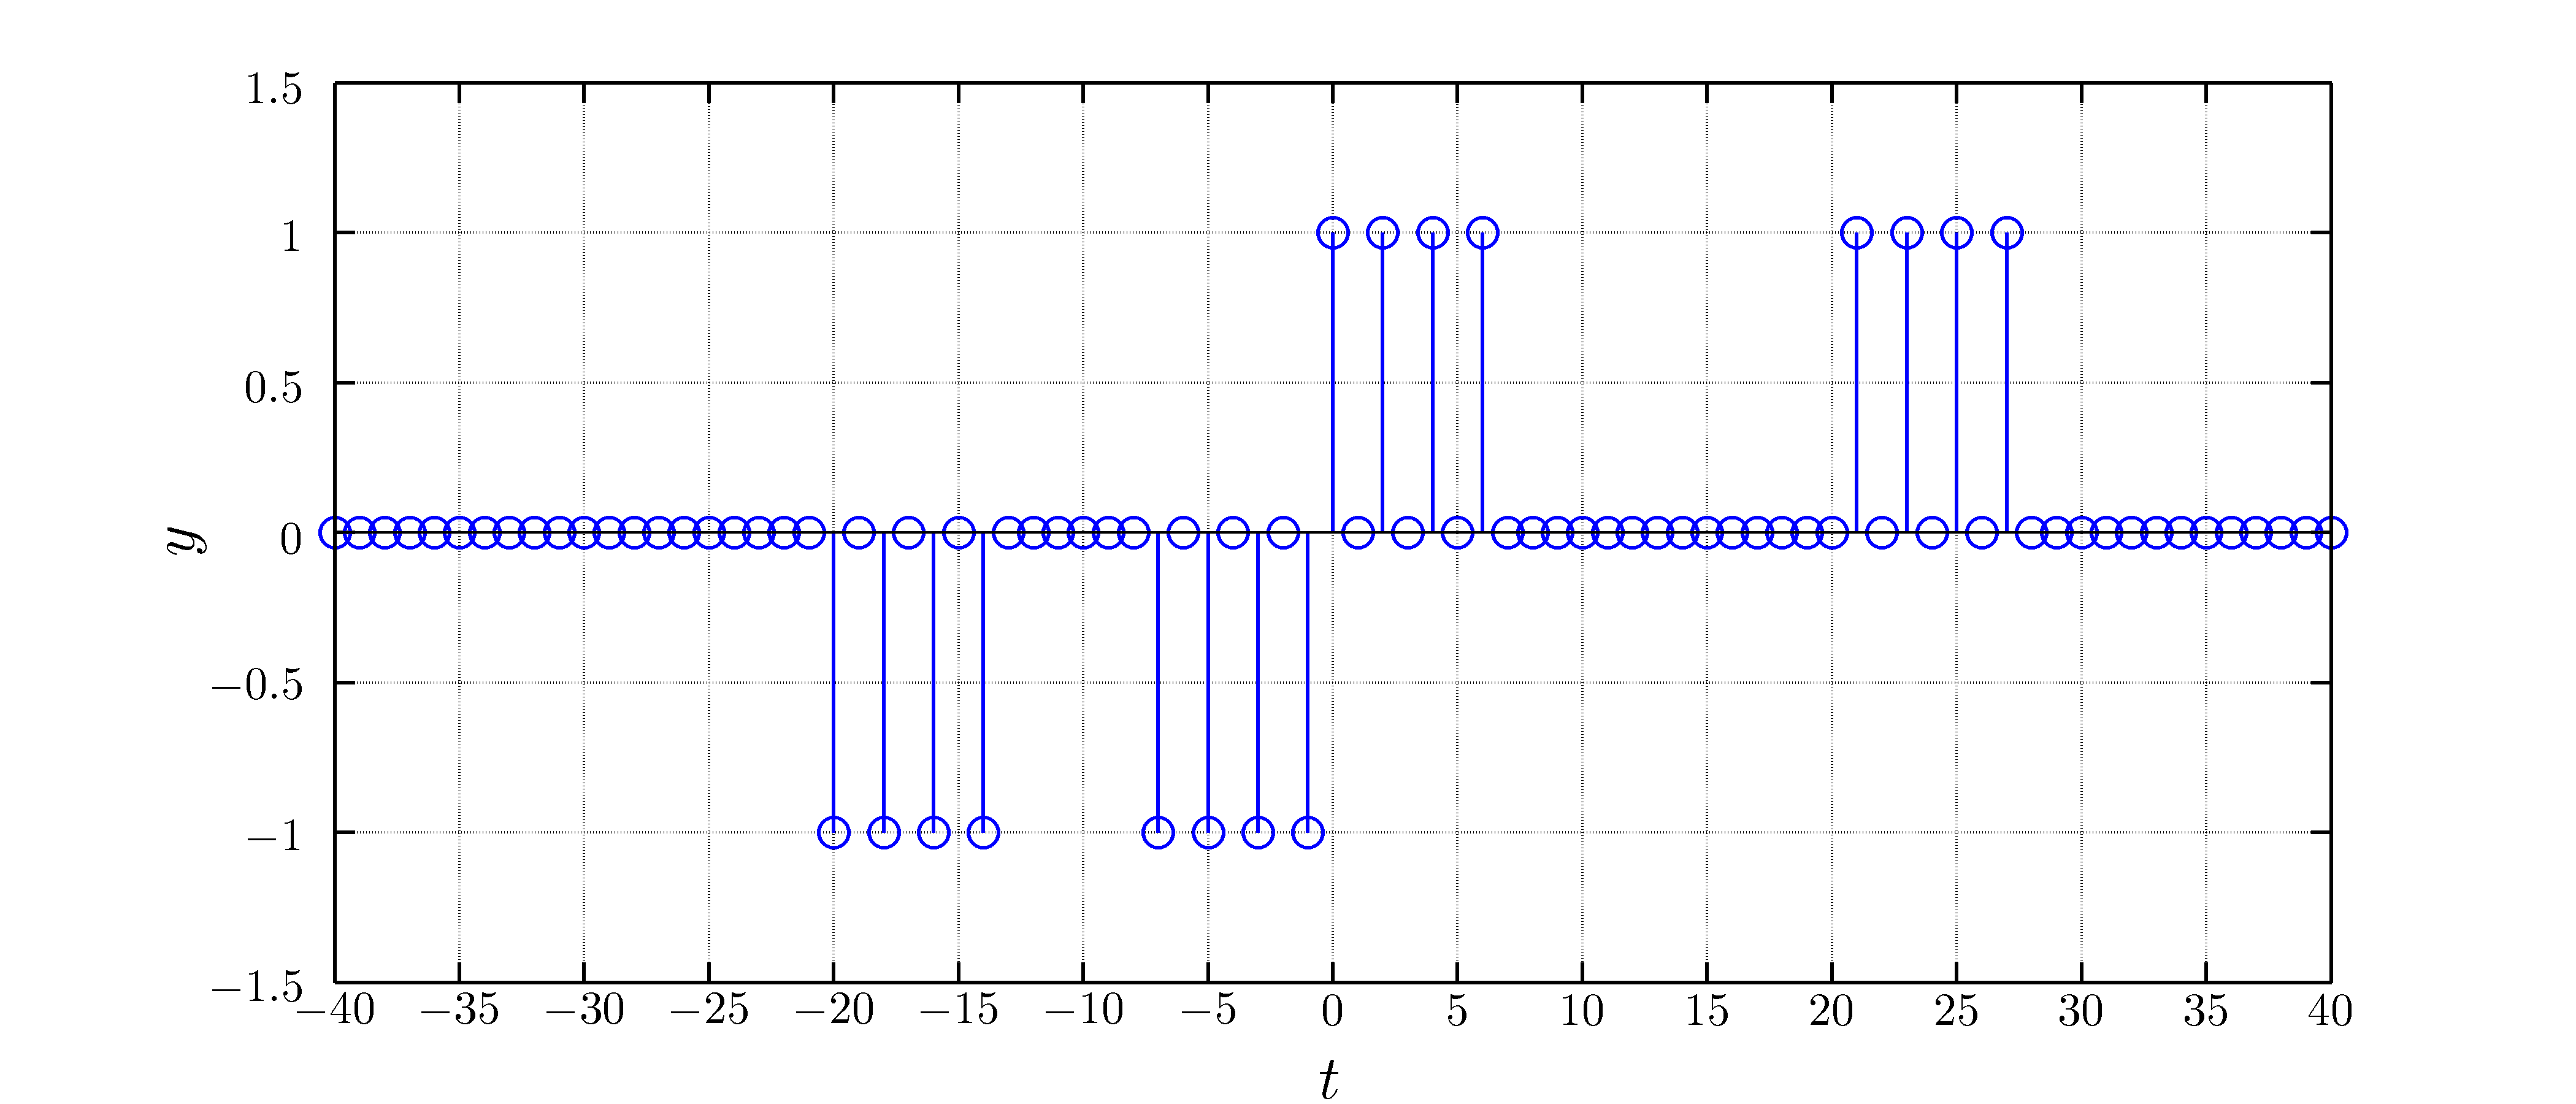
\includegraphics[width=0.90\textwidth]{./laboratorio_3/problema06_conv.png}
      \end{center}
    \end{figure}

  \newpage
  \subsection*{Problema 7}
    \noindent Considere un sistema lineal e invariante en el tiempo, causal,
    cuya entrada $x\left(n\right)$ y salida $y\left(n\right)$ estén
    relacionadas por la ecuación de diferencias:

    $$y\left(n\right) = 0.25 y\left(n-1\right) + x\left(n\right)$$

    Determine $y\left(n\right)$ si $x\left(n\right) = \delta\left(n-1\right)$.

    Grafique en \textsc{Matlab} la salida $y\left(n\right)$, use el comando \texttt{stem}.

    \subsubsection*{Solución}
      \noindent Para $n = 1$ tenemos

      \begin{equation*}
        \begin{split}
          y\left(1\right) & = 0.25 y\left(0\right) + x\left(1\right) \\
                          & = 0.25 y\left(0\right) + \delta\left(0\right) \\
                          & = 0.25 y\left(0\right) + 1
        \end{split}
      \end{equation*}

      \noindent Suponiendo que la señal $y\left(n\right)$ es nula antes antes de
      $n=1$ tenemos

      \begin{equation*}
        \begin{split}
          y\left(0\right) & = 0 \\
          y\left(1\right) & = 1
        \end{split}
      \end{equation*}

      \noindent Con estos valores en la definición de $y\left(n\right)$ obtenemos que

      $$y\left(n\right) = \frac{1}{4^{n-1}}u\left(n-1\right)$$

      \noindent La implementación y la gráfica que se obtienen de \textsc{Matlab}
      se muestran en el \emph{script  \ref{script07A}} y la
      \emph{script \ref{script07Afigure}} respectivamente.

      \begin{listing}[H]
        \caption{Función $y\left(n\right)$}
        \label{script07A}
        \inputminted{matlab}{./laboratorio_3/p7_Y.m}
      \end{listing}

      \begin{figure}[H]
        \caption{Gráfico de la función $y\left(n\right)$ calculada \emph{figura \ref{script07A}}.}
        \label{script07Afigure}
        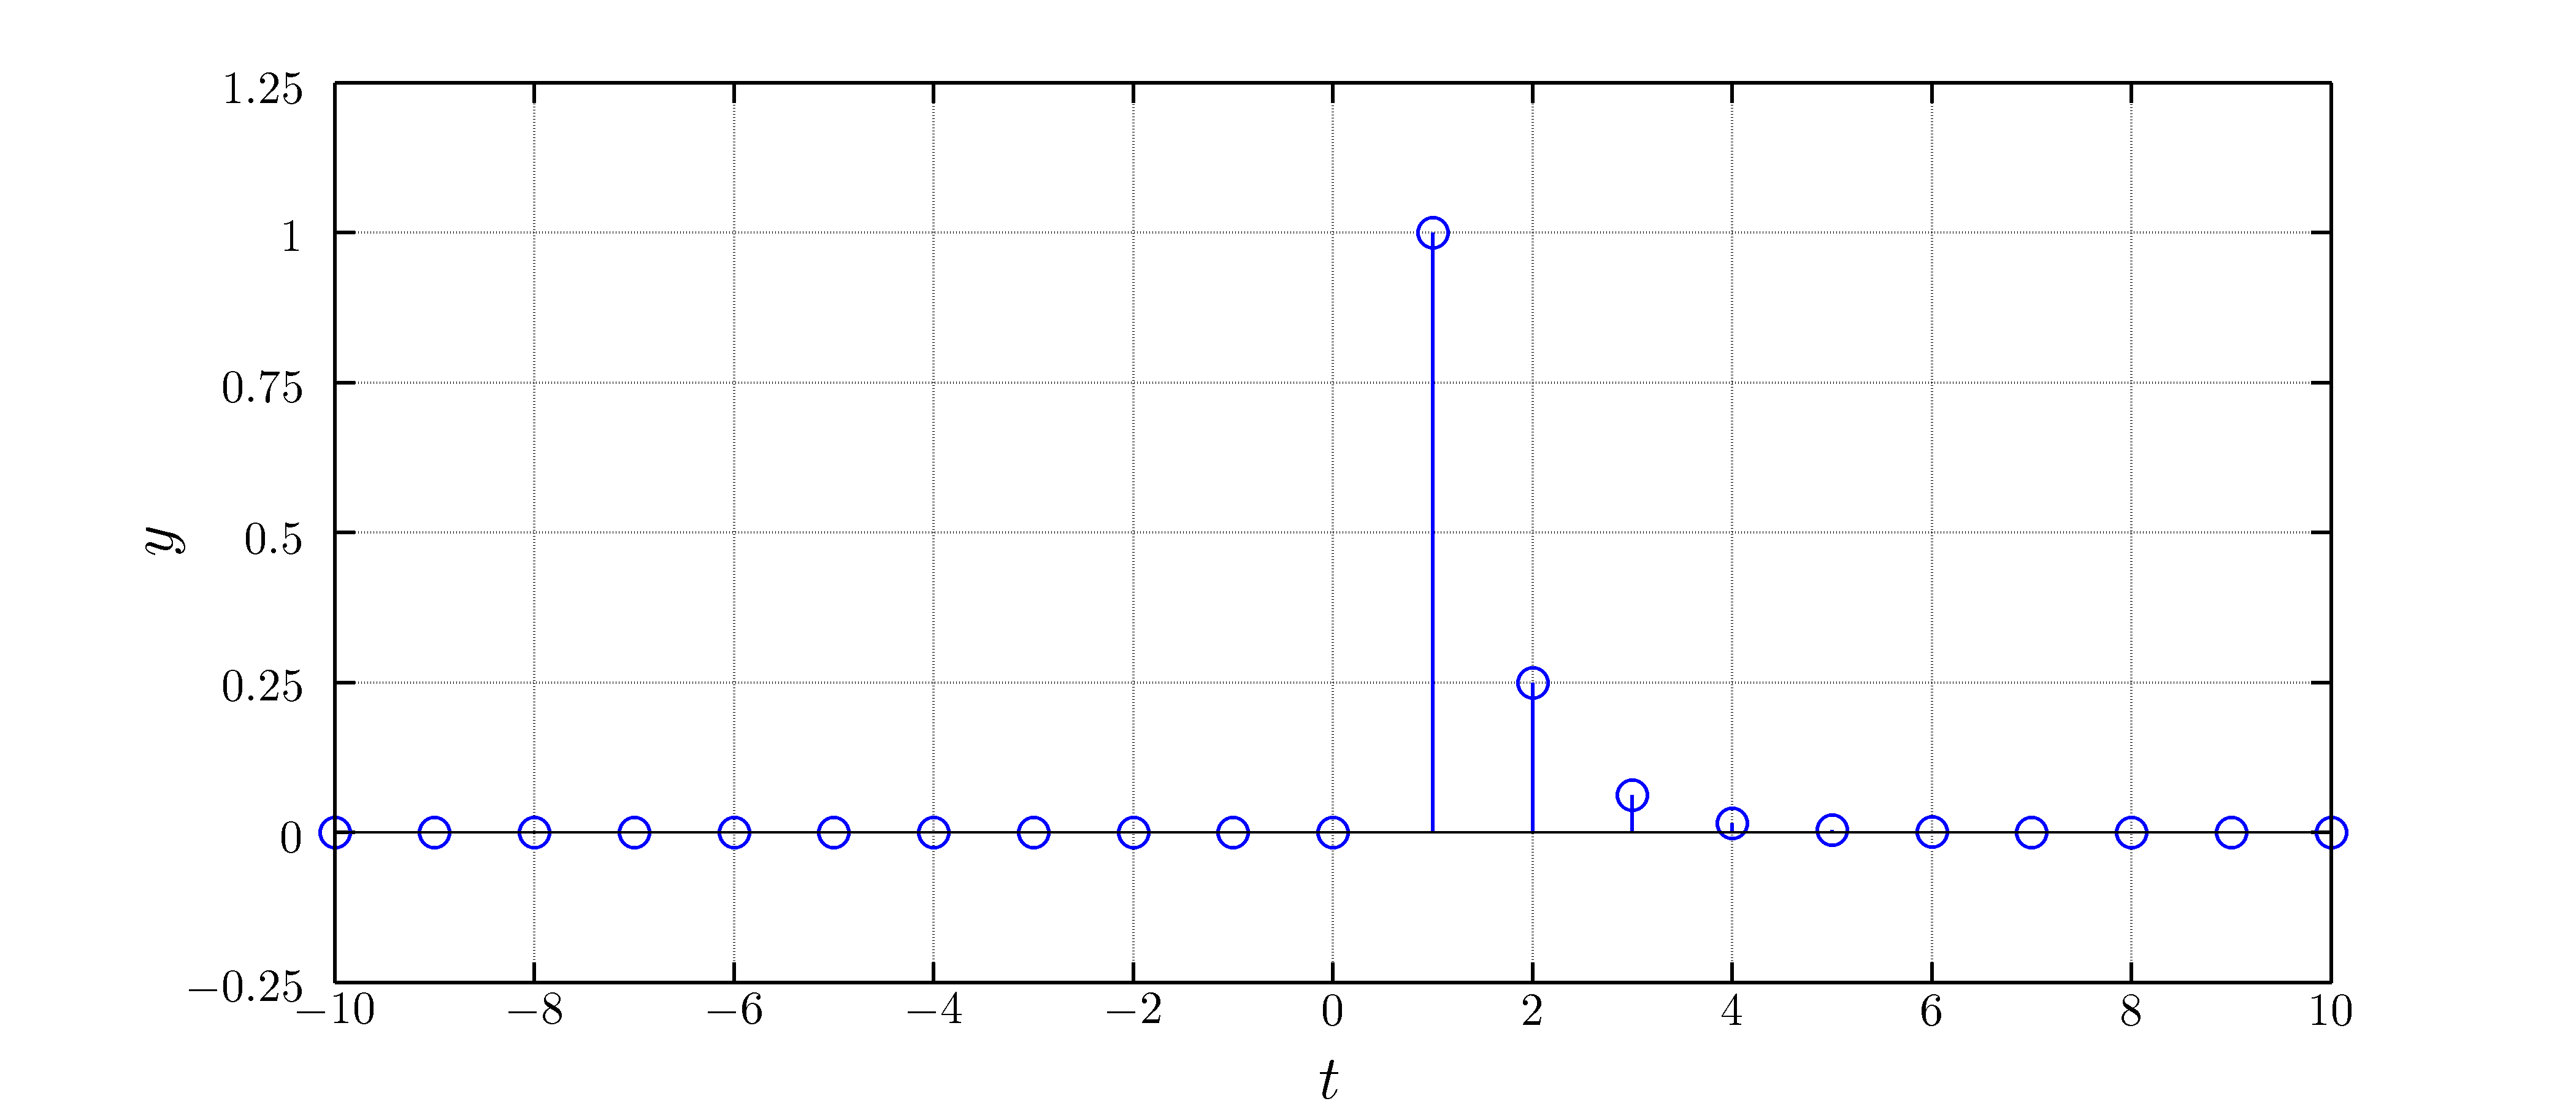
\includegraphics[width=0.90\textwidth]{./laboratorio_3/problema07_Y.png}
      \end{figure}

\end{document}
